\PassOptionsToPackage{dvipsnames}{xcolor}
\documentclass[a4paper,11pt]{report} %article

\usepackage{graphicx,subfigure,afterpage,hyperref,xspace,xcolor,caption,soul,geometry,pdfpages,stackengine,eso-pic,fancyhdr,hyphenat,listings,longtable}


%\usepackage[utf8]{inputenc} %to make the single quote appear correct after the encoding inserted above!

%command to substitute "{\em MyTaxyService}" with "\mts"
\newcommand{\mts}{\mbox{\normalfont\itshape myTaxiService}}
\geometry{margin=1in}

%header & footer style
\fancyhead{}
\fancyhead[C]{\iffloatpage{}{\slshape\rightmark}}
\fancyfoot{}
\fancyfoot[C]{\iffloatpage{}{\thepage}}
\renewcommand{\headrulewidth}{\iffloatpage{0pt}{0.4pt}}
\renewcommand{\footrulewidth}{\iffloatpage{0pt}{0.4pt}}
\pagestyle{fancy}
\renewcommand{\sectionmark}[1]{\markright{\thesection.\ #1}}
\renewcommand{\subsectionmark}[1]{\markright{\thesubsection.\ #1}}

%tOC style: sections bold 
\usepackage[subfigure]{tocloft}
\renewcommand{\cftsecfont}{\bfseries}
\renewcommand{\cftsecpagefont}{\normalfont\bfseries}% page numbers in bold
\renewcommand{\cftdotsep}{1}
\renewcommand{\cftsecleader}{\bfseries\cftdotfill{\cftsecdotsep}}% dot leaders in bold

%to keep the links of the TOC invisible
\hypersetup{
	colorlinks,
	citecolor=black,
	filecolor=black,
	linkcolor=black,
	urlcolor=black
}


\title{Politecnico di Milano\\A.A. 2015/2016\\Software Engineering 2: ``{\em myTaxyService}'' \\ \bigskip 
\textbf{D}esign \textbf{D}ocument}
\author{Alessandro Baldassari (mat. 841561) \\ Alberto Bendin (mat. 841734) \\ Francesco Giarola (mat. 840554)}


%to set the nested bullet lists style
\renewcommand{\labelitemii}{$\circ$}
%\renewcommand{\labelitemii}{}
\renewcommand{\labelitemiii}{$\diamond$}

%to avoid the hyphenation of the name of the software
\hyphenation{myTaxyService}

\begin{document}
	
	%fIRSTPAGE
	
	%pOLIMI-LOGO
	\begin{figure}[t]
		\centering
		\includegraphics[width=1\linewidth]{"Pictures/polimi-logo"}
		\label{fig:polimi-logo}
	\end{figure}
	
	\maketitle
		
	
	%bLANK-PAGE
	\thispagestyle{empty}
	\clearpage\mbox{}\clearpage

	
	
	
	%to number the section from 1 instead of 0.1 with the report class, without using the article class. Avoid the forced use of chapters to number from 1. Tailored for REPORT class!!!
	\renewcommand*\thesection{\arabic{section}}
	\renewcommand*\thesubsection{\arabic{section}.\arabic{subsection}}
	\renewcommand*\thesubsubsection{%
	\arabic{section}.\arabic{subsection}.\arabic{subsubsection}%
	}
	\setcounter{secnumdepth}{4}
	\setcounter{tocdepth}{4}
		
	
	%to change the page numbering from roman in the toc to arabic
	\pagenumbering{roman}
	\tableofcontents
	\newpage
	\pagenumbering{arabic}
	
	
	%to insert the writing "Page" above page numbers in the TOC
	\addtocontents{toc}{~\hfill\textrm{Page}\par}
	
	\section{Introduction}
	
	\subsection{Purpose} This document presents the architecture on which \mts{} will be developed; it describes the decisions taken during the design process and justifies them. The whole process is reported, including the improvements and modifications, this is to provide additional valuable information in case of future changes of the architecture structure.
	
	\subsection{Scope} Accordingly to the definition of the architecture design, this document will focus on the non-functional requirements of \mts{}. 
	Since the system architecture  defines constraints on the implementation this document will  be  used to provide fundamental guidelines in the development phase of \mts{}.
%	The system architecture will be organized in three categories corresponding to the functionalities of the different users: passengers, drivers and administrator.
%	\begin{itemize}
%		\item \textbf{Passengers} \\
%		The system allows the user to sign up, login, request or reserve a taxi with the customization of the ride. 
%		\item \textbf{Taxi drivers} \\
%		The system allows the user to login, set the ``availability'' and accept or reject jobs.
%		\item \textbf{Administrator} \\
%		The system allows the user to login, manage the drivers' list and supervise the system itself.
%	\end{itemize}
	
	\subsection{Definitions, Acronyms, Abbreviations}
	The following acronyms are used in this document:
	\begin{itemize}
		\item JEE: Java Enterprise Edition
		\item RASD: Requirements Analysis and Specification Document
		\item UI: User Interface
		\item EIS: Enterprise Information System
		\item API: Application Programming Interface
	\end{itemize}
	The following definitions are used in this document:
	\begin{itemize}
		\item Thin client: is a computer that depends heavily on another computer (its server) to fulfill its computational roles.
		\item Fat server: is a type of server that provides most of the functionality to a client's machine within a client/server computing architecture.
		\item Event-driven architecture:  is a software architecture pattern promoting the production, detection, consumption of, and reaction to events, that is a change of state of an object.
		\item Availability: is the ``status'' of a taxi driver, s/he can be \textit{waiting} (available) to take care of new jobs, thus the system should forward compatible requests, or can be \textit{offline} (unavailable), meaning that the taxi is temporarily off line with respect to the system, thus the system should not consider that taxi for requests assignment. The driver can also be \textit{working} (busy), as a third ``status'', that is when s/he is carrying passengers.
	\end{itemize}
	
	\subsection{Reference Documents}
	\begin{itemize}
		\item Specification document: myTaxiService project
		\item Template for the Design Document
		\item IEEE Std 1016™-2009 - IEEE Standard on Design Descriptions
		\item Requirements Analysis and Specification Document (RASD) for \mts{}
	\end{itemize}
	
	\subsection{Document Structure} This  document  specifies  the  architecture  of  the  system  using  different levels of detail. It also describes the architectural decisions and justifies them. The design is  developed  in  a  top-­‐down  way, then the  document  reflects this approach.
	The document is organized in the following sections:
	\begin{enumerate}
		\item Introduction\\
		Provides a synopsis of the architectural descriptions.
		\item Architectural design\\
		It is the core of the design document, here are presented all the components of the system and the interaction between them in increasing level of detail starting from an high-level overview.		
		\item Algorithm design\\
		Flowchart and pseudocode description of the fundamental algorithms of \mts{}. 
		\item User interface design\\
		Some mock-ups of the UI to better understand how the functionalities have been implemented from a graphical viewpoint.
		\item Requirements traceability\\
		Presents the mapping between the requirements and the components used to satisfy them.
		\item References\\
		List of sources for material used in this document: internet links, books.
		
	\end{enumerate} 
	
	\pagebreak
	\section{Architectural Design}
	
	\subsection{Overview} This  section  of  the  design  document  provides  a  general  description  of  the  design  of  the  system  and  its  processes.\\
	The architectural style adopted by \mts{} is the well-known ``client-server'', where the client is a ``thin client'' and the server is a ``fat server''. The architecture is ``event-driven'', thus the interaction between the components takes place through events, in other words asynchronous triggers. \\	
	JEE has a ``four-tier'' architecture divided as shown in the picture below:\\
		\begin{minipage}{\linewidth}
%			\vspace*{-0.35cm}
			\makebox[\linewidth]{
				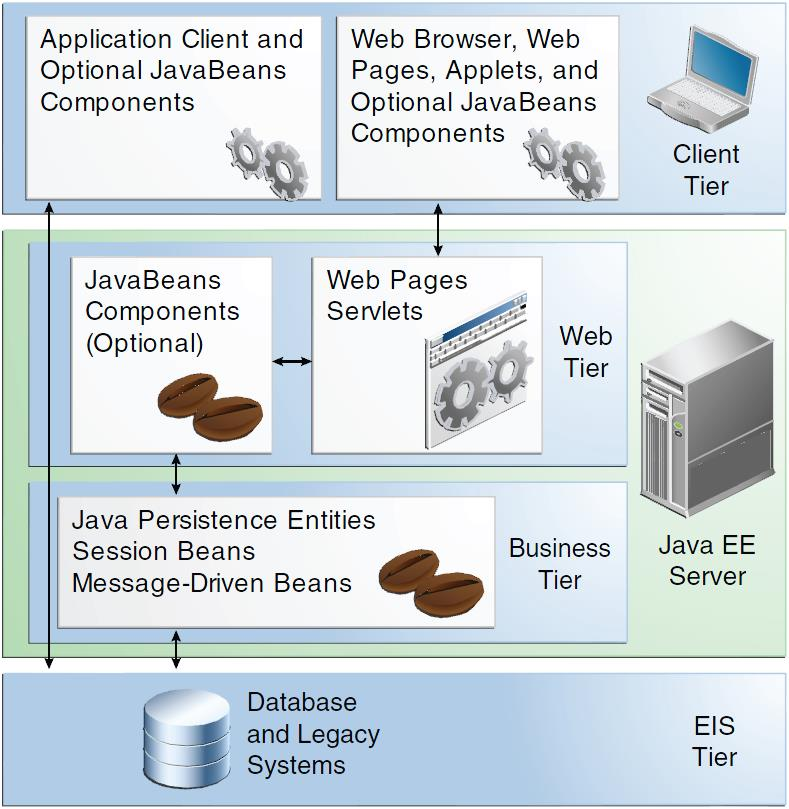
\includegraphics[keepaspectratio=true,scale=0.57]{Pictures/4tier}}
		\end{minipage}	
		\begin{enumerate}
			\item \textbf{Client Tier}: contains Application Clients and Web Browsers and it is the layer designed to interact directly with the users. \mts{} is a web and mobile application, then the client will use a web browser or a smartphone to access the pages.
			\item \textbf{Web Tier}: contains the Servlets and Dynamic Web Pages that need to be elaborated. This tier receives the requests from the client tier and forwards the pieces of data collected to the business tier; it also works in the opposite direction waiting for processed data correctly formatted to be sent to the client tier.
			\item \textbf{Business Tier}: contains the Java Beans, which contain the business logic of the application, and Java Persistence Entities.
			\item \textbf{EIS Tier}: contains the data source. In our case, it is the database allowed to store all the relevant data and to retrieve them.									
		\end{enumerate}
	When the second and third tier are considered together the architecture becomes a ``three-tier'' with \textit{client tier}, \textit{business logic tier} and \textit{persistence tier}.\\
	To design the system a top-­‐down approach is used. After the identification of the main three layers, the system is decomposed in components that capture subsets of related functionalities. For each component is specified the role in the architecture and its interactions with the rest of the system. 
	
	\subsubsection{Identifying sub-systems} The functionalities of \mts{} are divided into these functional areas:
	
	\begin{itemize}
		\renewcommand{\labelitemii}{}
		\item myTaxiService
		\begin{itemize}
			\item This component describes the system that is going to be developed.
		\end{itemize} 
		\item Users
		\begin{itemize}
			\item This component represents all the users that will use the service.
		\end{itemize}
		\item Notification service
		\begin{itemize}
			\item This component represents the notification mechanism that the system will use (text-messages, emails and push notifications).
		\end{itemize}
		\item Payment service
		\begin{itemize}
			\item This component represents the external service in charge of managing the payments.
		\end{itemize}
		\item Third party apps
		\begin{itemize}
			\item This component represents generally the external apps that can possibly connect to the system via our public web APIs.
		\end{itemize}
	\end{itemize}
	\renewcommand{\labelitemii}{$\circ$}
	The following schema shows the above-mentioned components and their interaction.\\
	\begin{minipage}{\linewidth}
		\vspace*{0.35cm}
		\makebox[\linewidth]{
			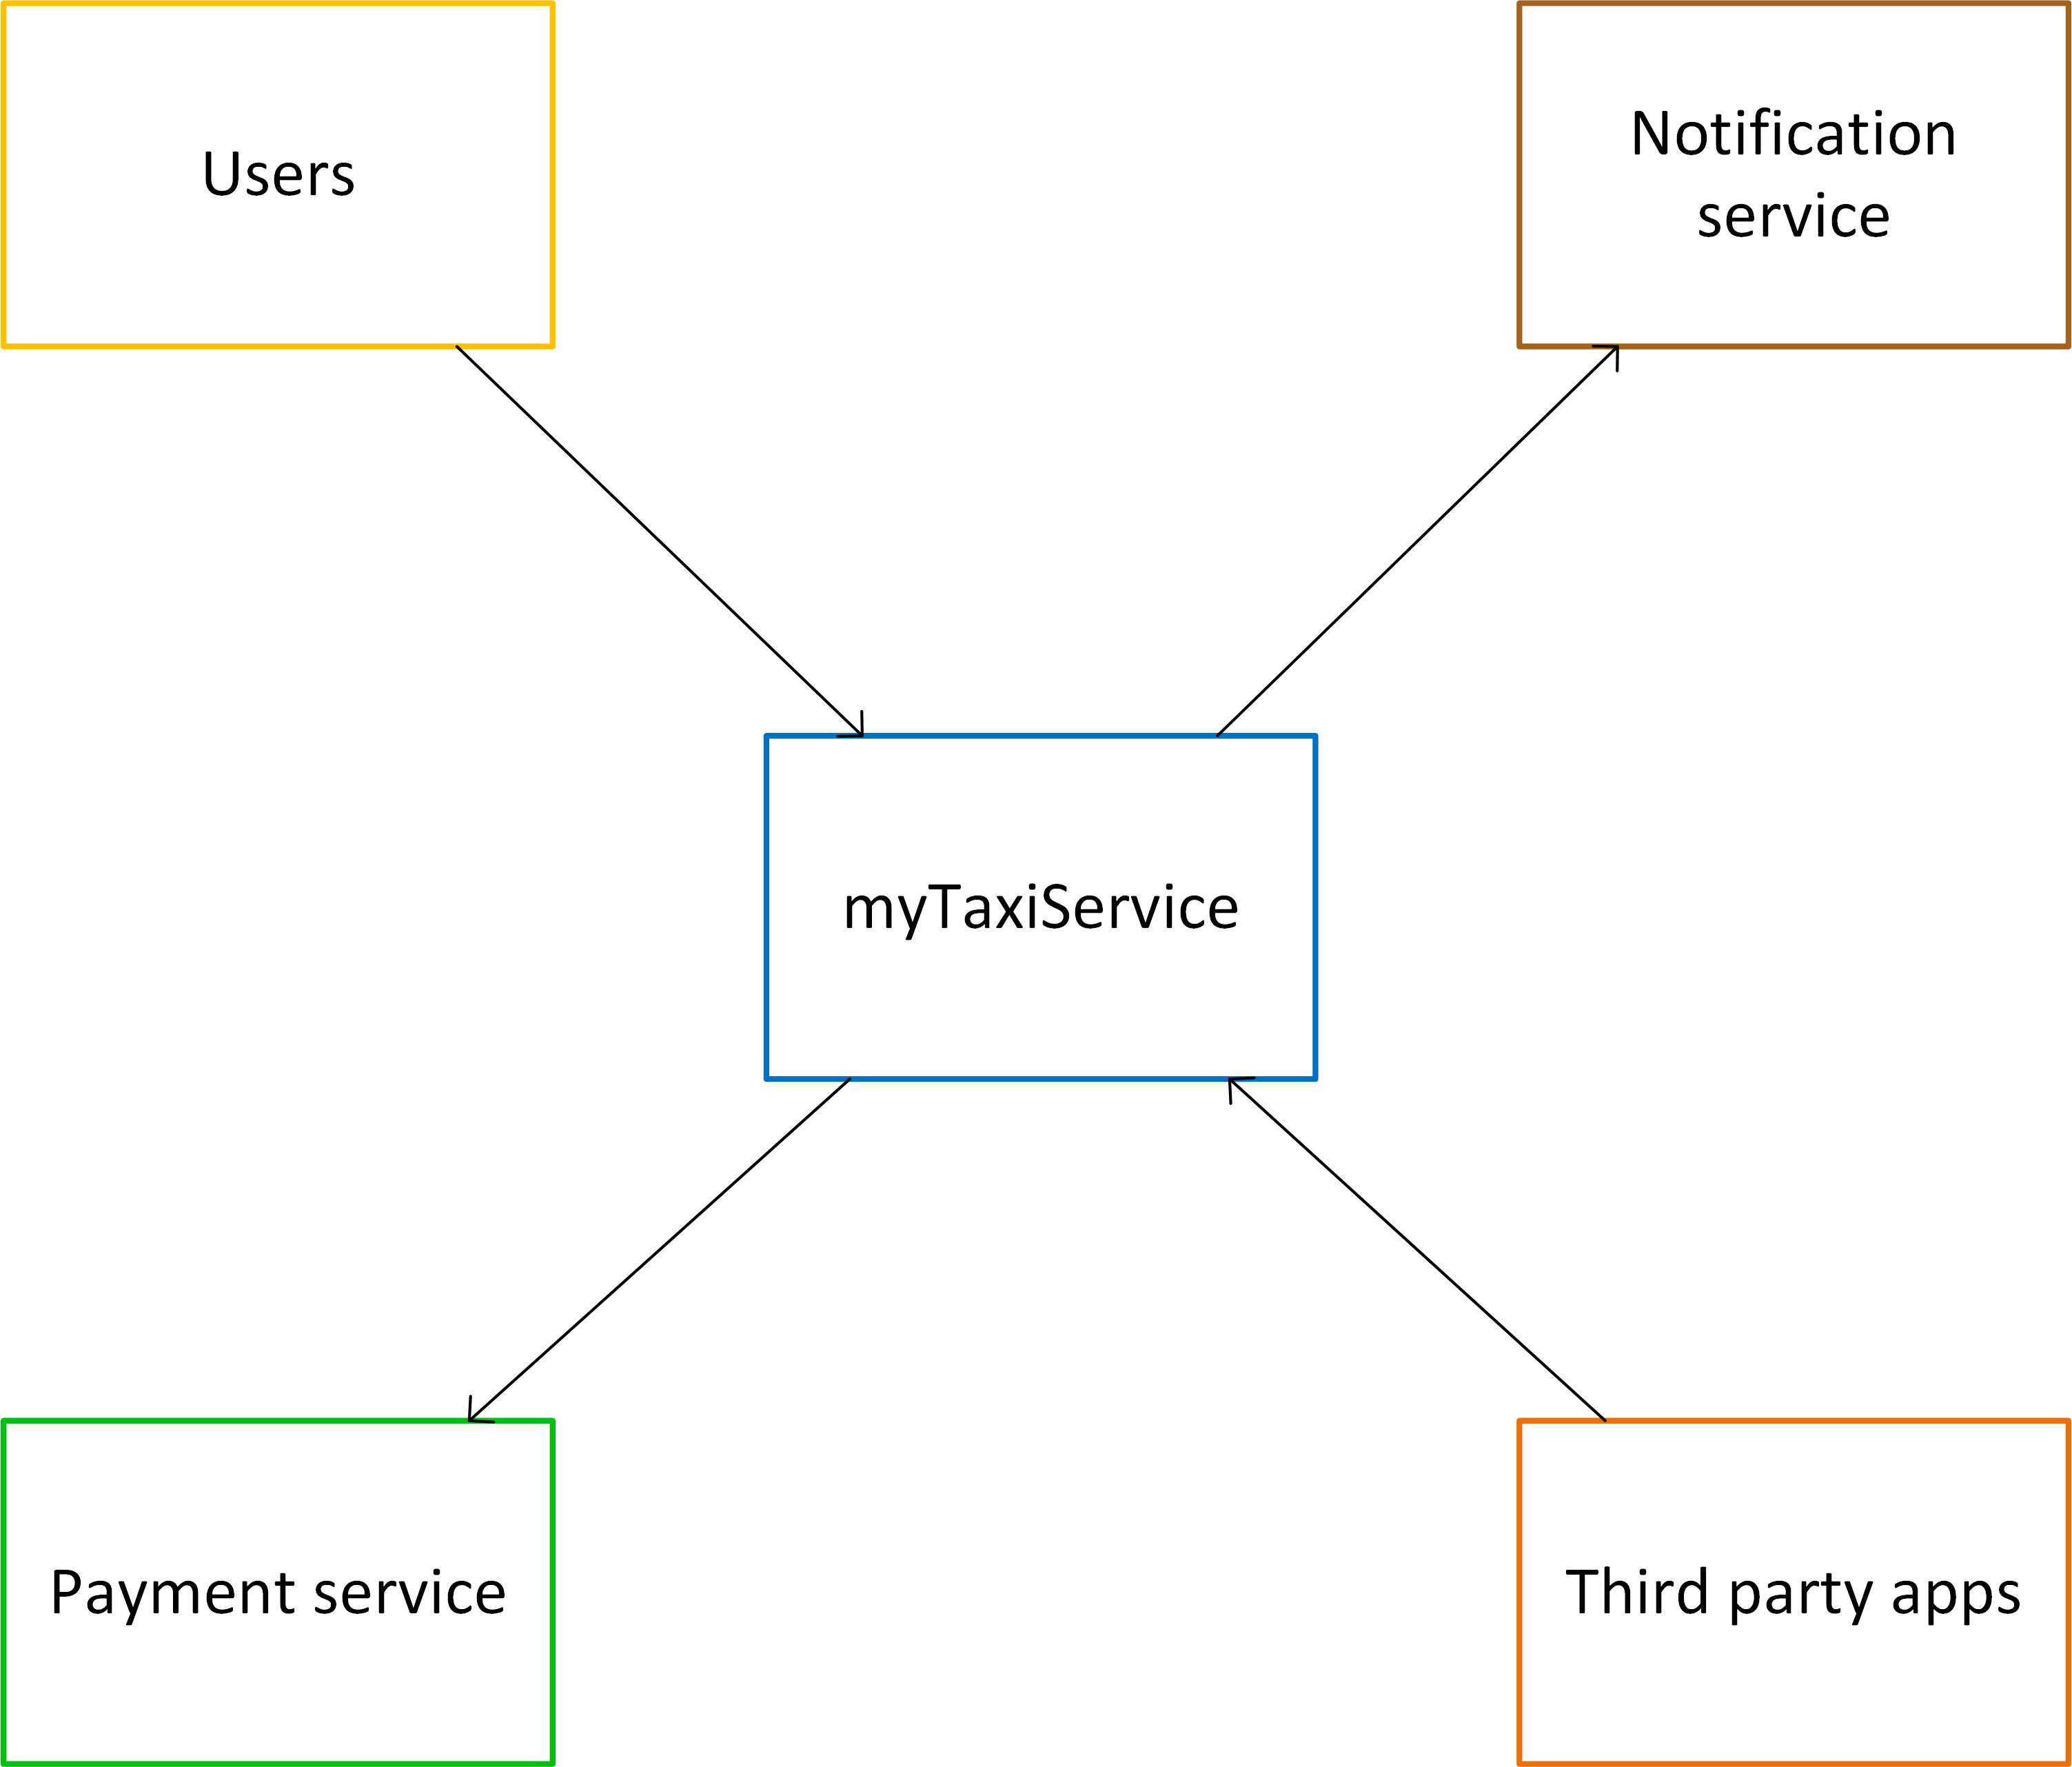
\includegraphics[keepaspectratio=true,scale=0.83]{Pictures/VisioSystemComponentsHighLevel}}
		\vspace{0.35cm}
	\end{minipage}
	
	The ``notification service'', ``payment service'' and ``third party apps'' are external components that are not part of the \mts{} system.	
	
	\subsection{High level components and their interaction} 
	

	
	\subsubsection{General Package design}
	Considering the three-tier view of the architecture three packages are identified: 
	\begin{itemize}
		\item User UI: this  package  is  in  charge  of  interacting  with  the  user; it  receives  the  user  requests, sends these to the business logic package, obtains the information needed from the latter and displays them to the user accordingly. In general the package contains the user interfaces.
		\item Business  logic: this package is in charge of receiving and processing the User UI's package requests, accessing the Persistence package when needed and sending a response accordingly. 
		\item Persistence: this package is in charge of managing the data requests from the Business logic package.
	\end{itemize}
	The  main  users:  administrator,  passengers  and  taxi  drivers  directly  access the  User  UI  package  but  cannot see the other packages, as shown in the picture below. \\
	\begin{minipage}{\linewidth}
%		\vspace*{-0.35cm}
		\makebox[\linewidth]{
		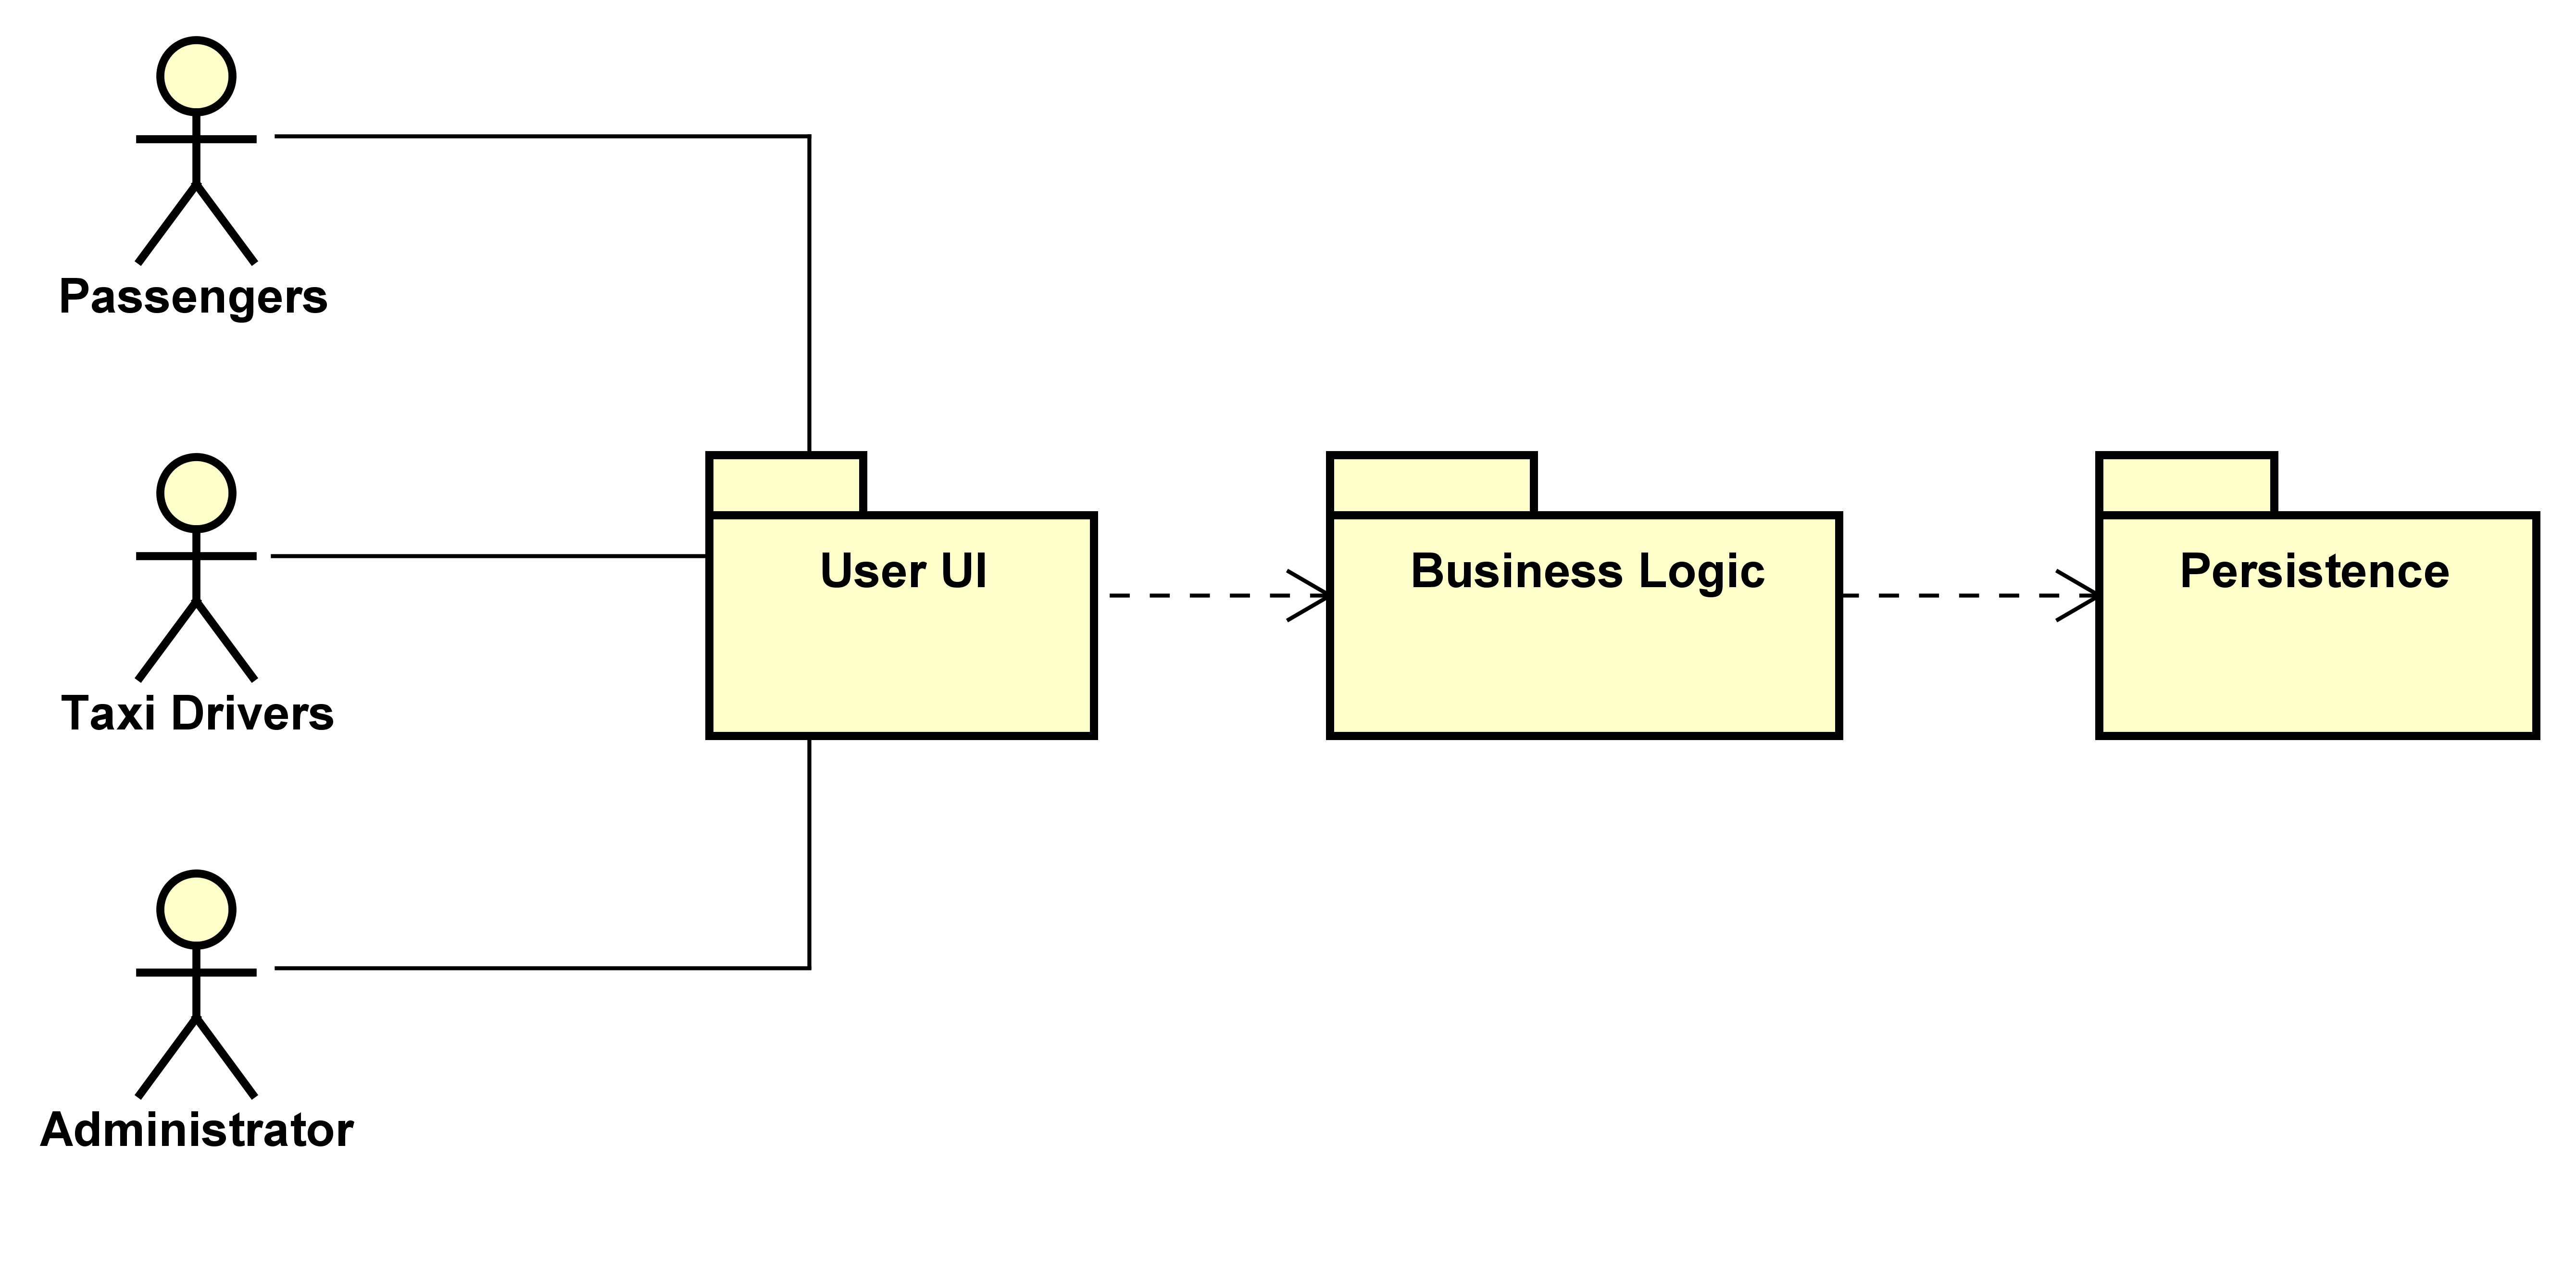
\includegraphics[keepaspectratio=true,scale=0.6]{Pictures/Packages}}
	\end{minipage}	
	
	\subsubsection{Detailed Package Design}
	The inner packages are described as follows:\\
	\begin{itemize}
		\item User UI:	this set of sub-packages is responsible for encapsulating the user's actions and forwarding information requests to the Business Logic sub-packages.
		\item Business logic: this set of sub-packages is responsible for handling requests from the User UI package, processing them and sending back a response. These packages may access the Persistence package.
		\item Persistence: this set of sub-packages contains the data model for the system. It accepts requests from the Business Logic package.
	\end{itemize}
	A more detailed view of the system from which is evident that all the controllers are part of the business logic:\\
	\begin{minipage}{\linewidth}
		%		\vspace*{-0.35cm}
		\makebox[\linewidth]{
			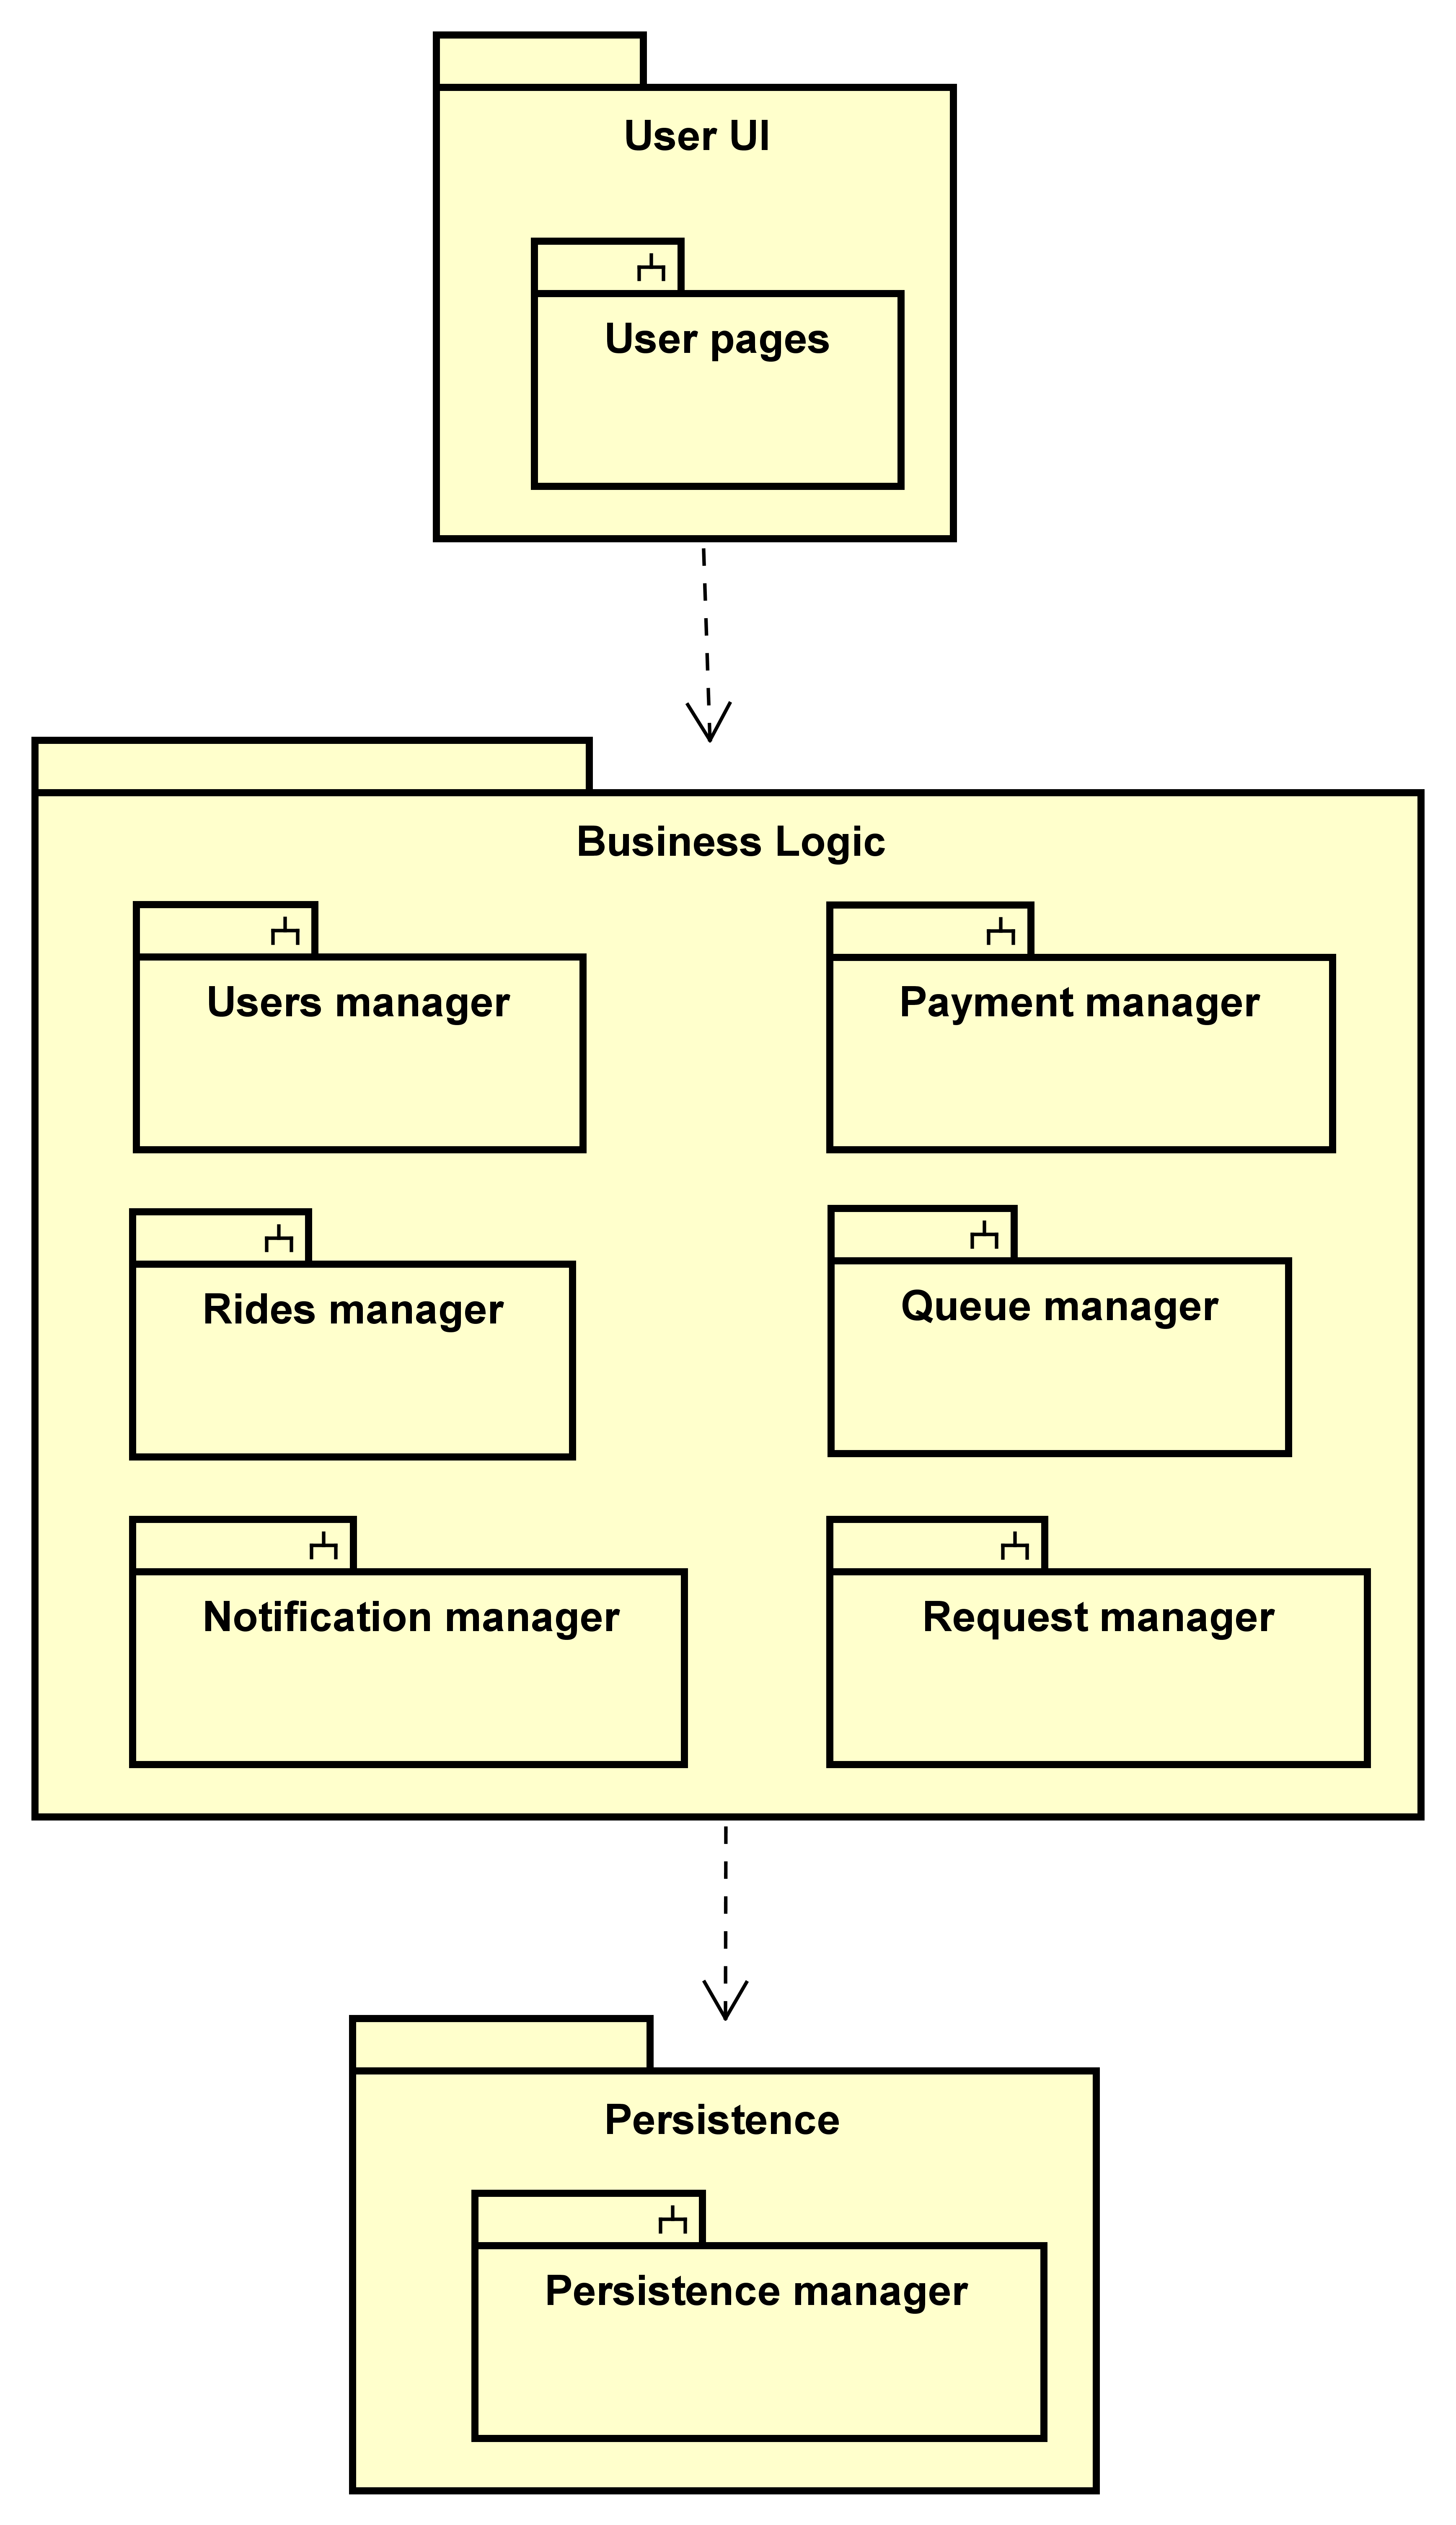
\includegraphics[keepaspectratio=true,scale=0.8]{Pictures/PackagesDetails}}
	\end{minipage}
	
	\subsubsection{High Level Component View}
	The picture below represents the main components and interfaces of \mts{}.\\
	\begin{minipage}{\linewidth}
		%		\vspace*{-0.35cm}
		\makebox[\linewidth]{
			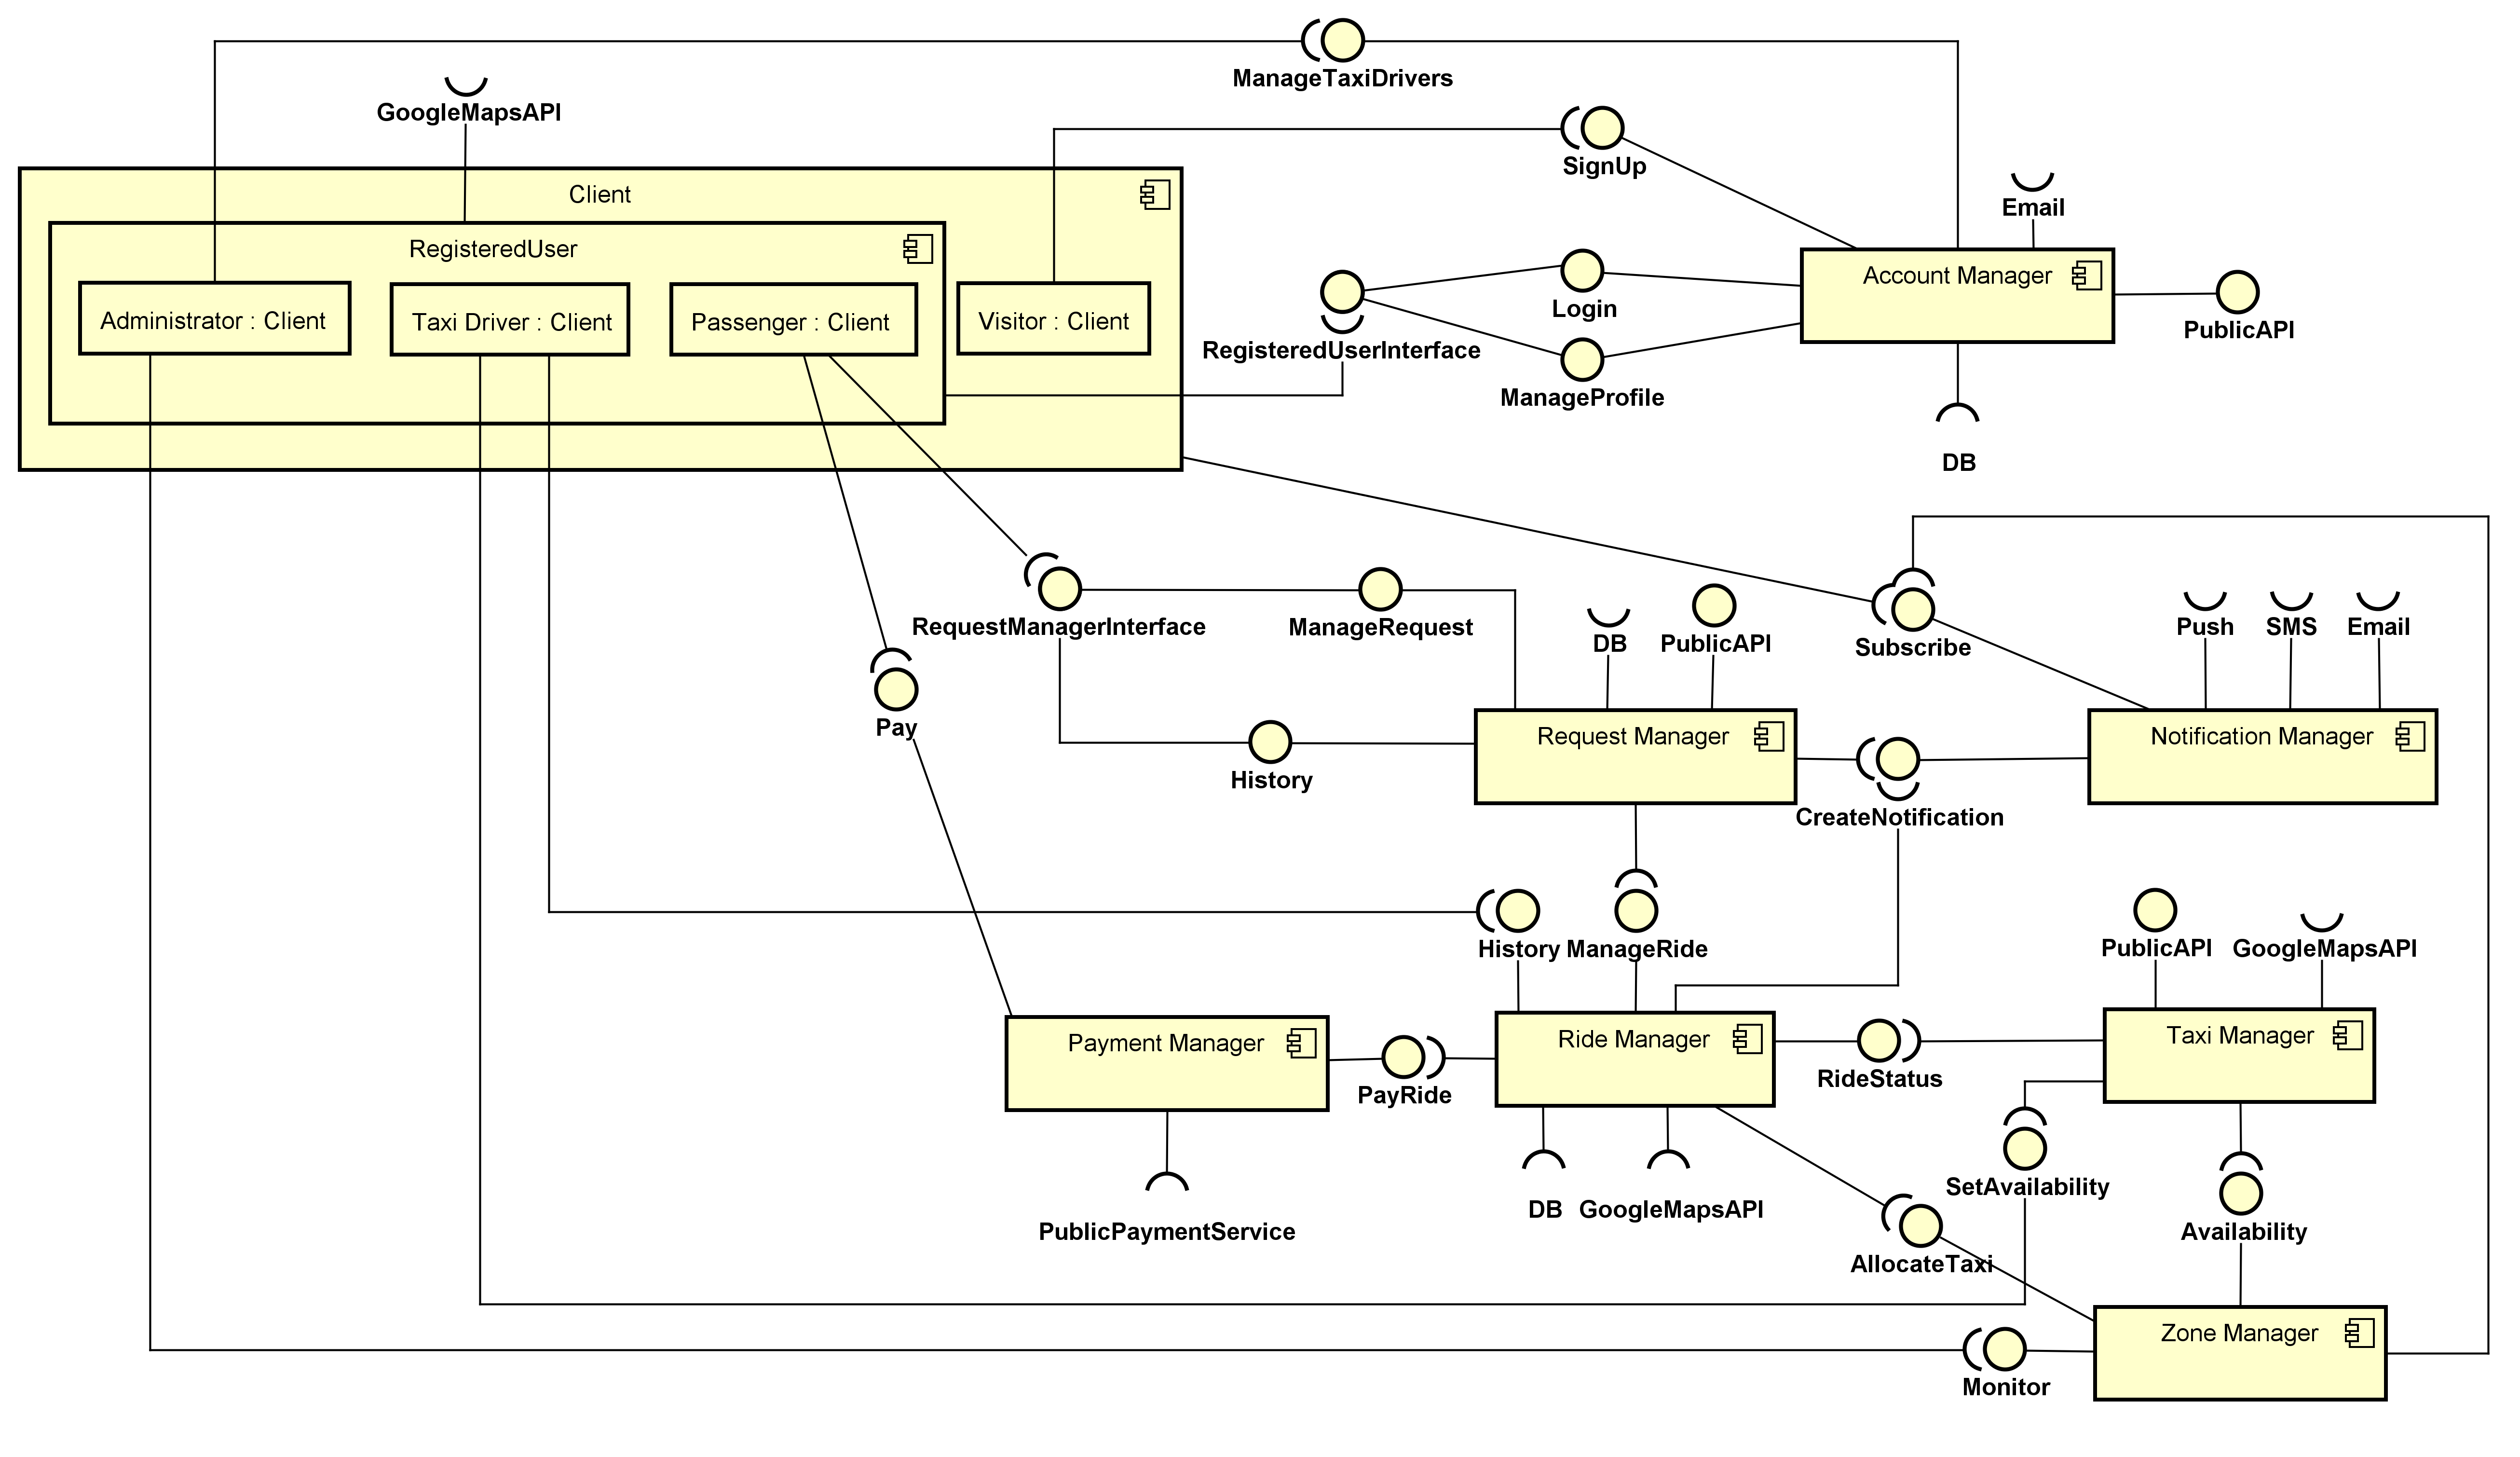
\includegraphics[keepaspectratio=true,scale=0.4]{Pictures/HighLevelComponent}}
	\end{minipage}		
	From the diagram above it is evident that:
	\begin{itemize}
		\renewcommand{\labelitemi}{$\Rightarrow$}
		\item The \textit{AccountManager} is the controller in charge of offering the sign-up functionality to the visitors, the login to all the different types of registered users; it also offers the functions related to the managing of the user's profile like ``changePassword'', ``changeNotificationType'' or ``updateCreditCardData''. It also enables the administrator to  manage the drivers list.
		\item The \textit{PaymentManager} is the interface in charge of exchanging the information about the transaction with the payment service provider.
		\item The \textit{RideManager} communicates with the \textit{RequestManager} to prepare the physical ride with the information collected by the latter.
		\item The \textit{ZoneManager} and \textit{TaxiManager} cooperate to assign the taxi to the zones in a fair way and to allocate drivers for the rides.
		\item The connection between the \textit{Administrator} and the \textit{ZoneManager} enables the administrator to supervise the situation of all the queues in real-time and the overall system.
		\item The \textit{NotificationManager} is connected to the \textit{RequestManager} to send passengers confirmation about creation/deletion of requests, it is connected with the ride manager for the same purpose, but in this case it can also warn taxi drivers about the ride they are currently working on.
		\item The two interfaces \textit{RequestManagerInterface} and \textit{RegisteredUserInterface} use the ``facade'' pattern to gather in one unique simpler interface the functionalities offered to the users in both the cases.
	\end{itemize}	
	
	\subsection{Component view and interfaces} Here is a more detailed view of every component with its interfaces.
	
	\renewcommand{\arraystretch}{1.5}
	\setlength{\tabcolsep}{6pt}
	
%	\subsubsection{User}
%	\begin{minipage}{\linewidth}
%		%		\vspace*{-0.35cm}
%		\makebox[\linewidth]{
%			\includegraphics[keepaspectratio=true,scale=0.4]{Pictures/CVUser}}
%	\end{minipage}	
		
	\subsubsection{Account Manager}
	\begin{minipage}{\linewidth}
		%		\vspace*{-0.35cm}
		\makebox[\linewidth]{
			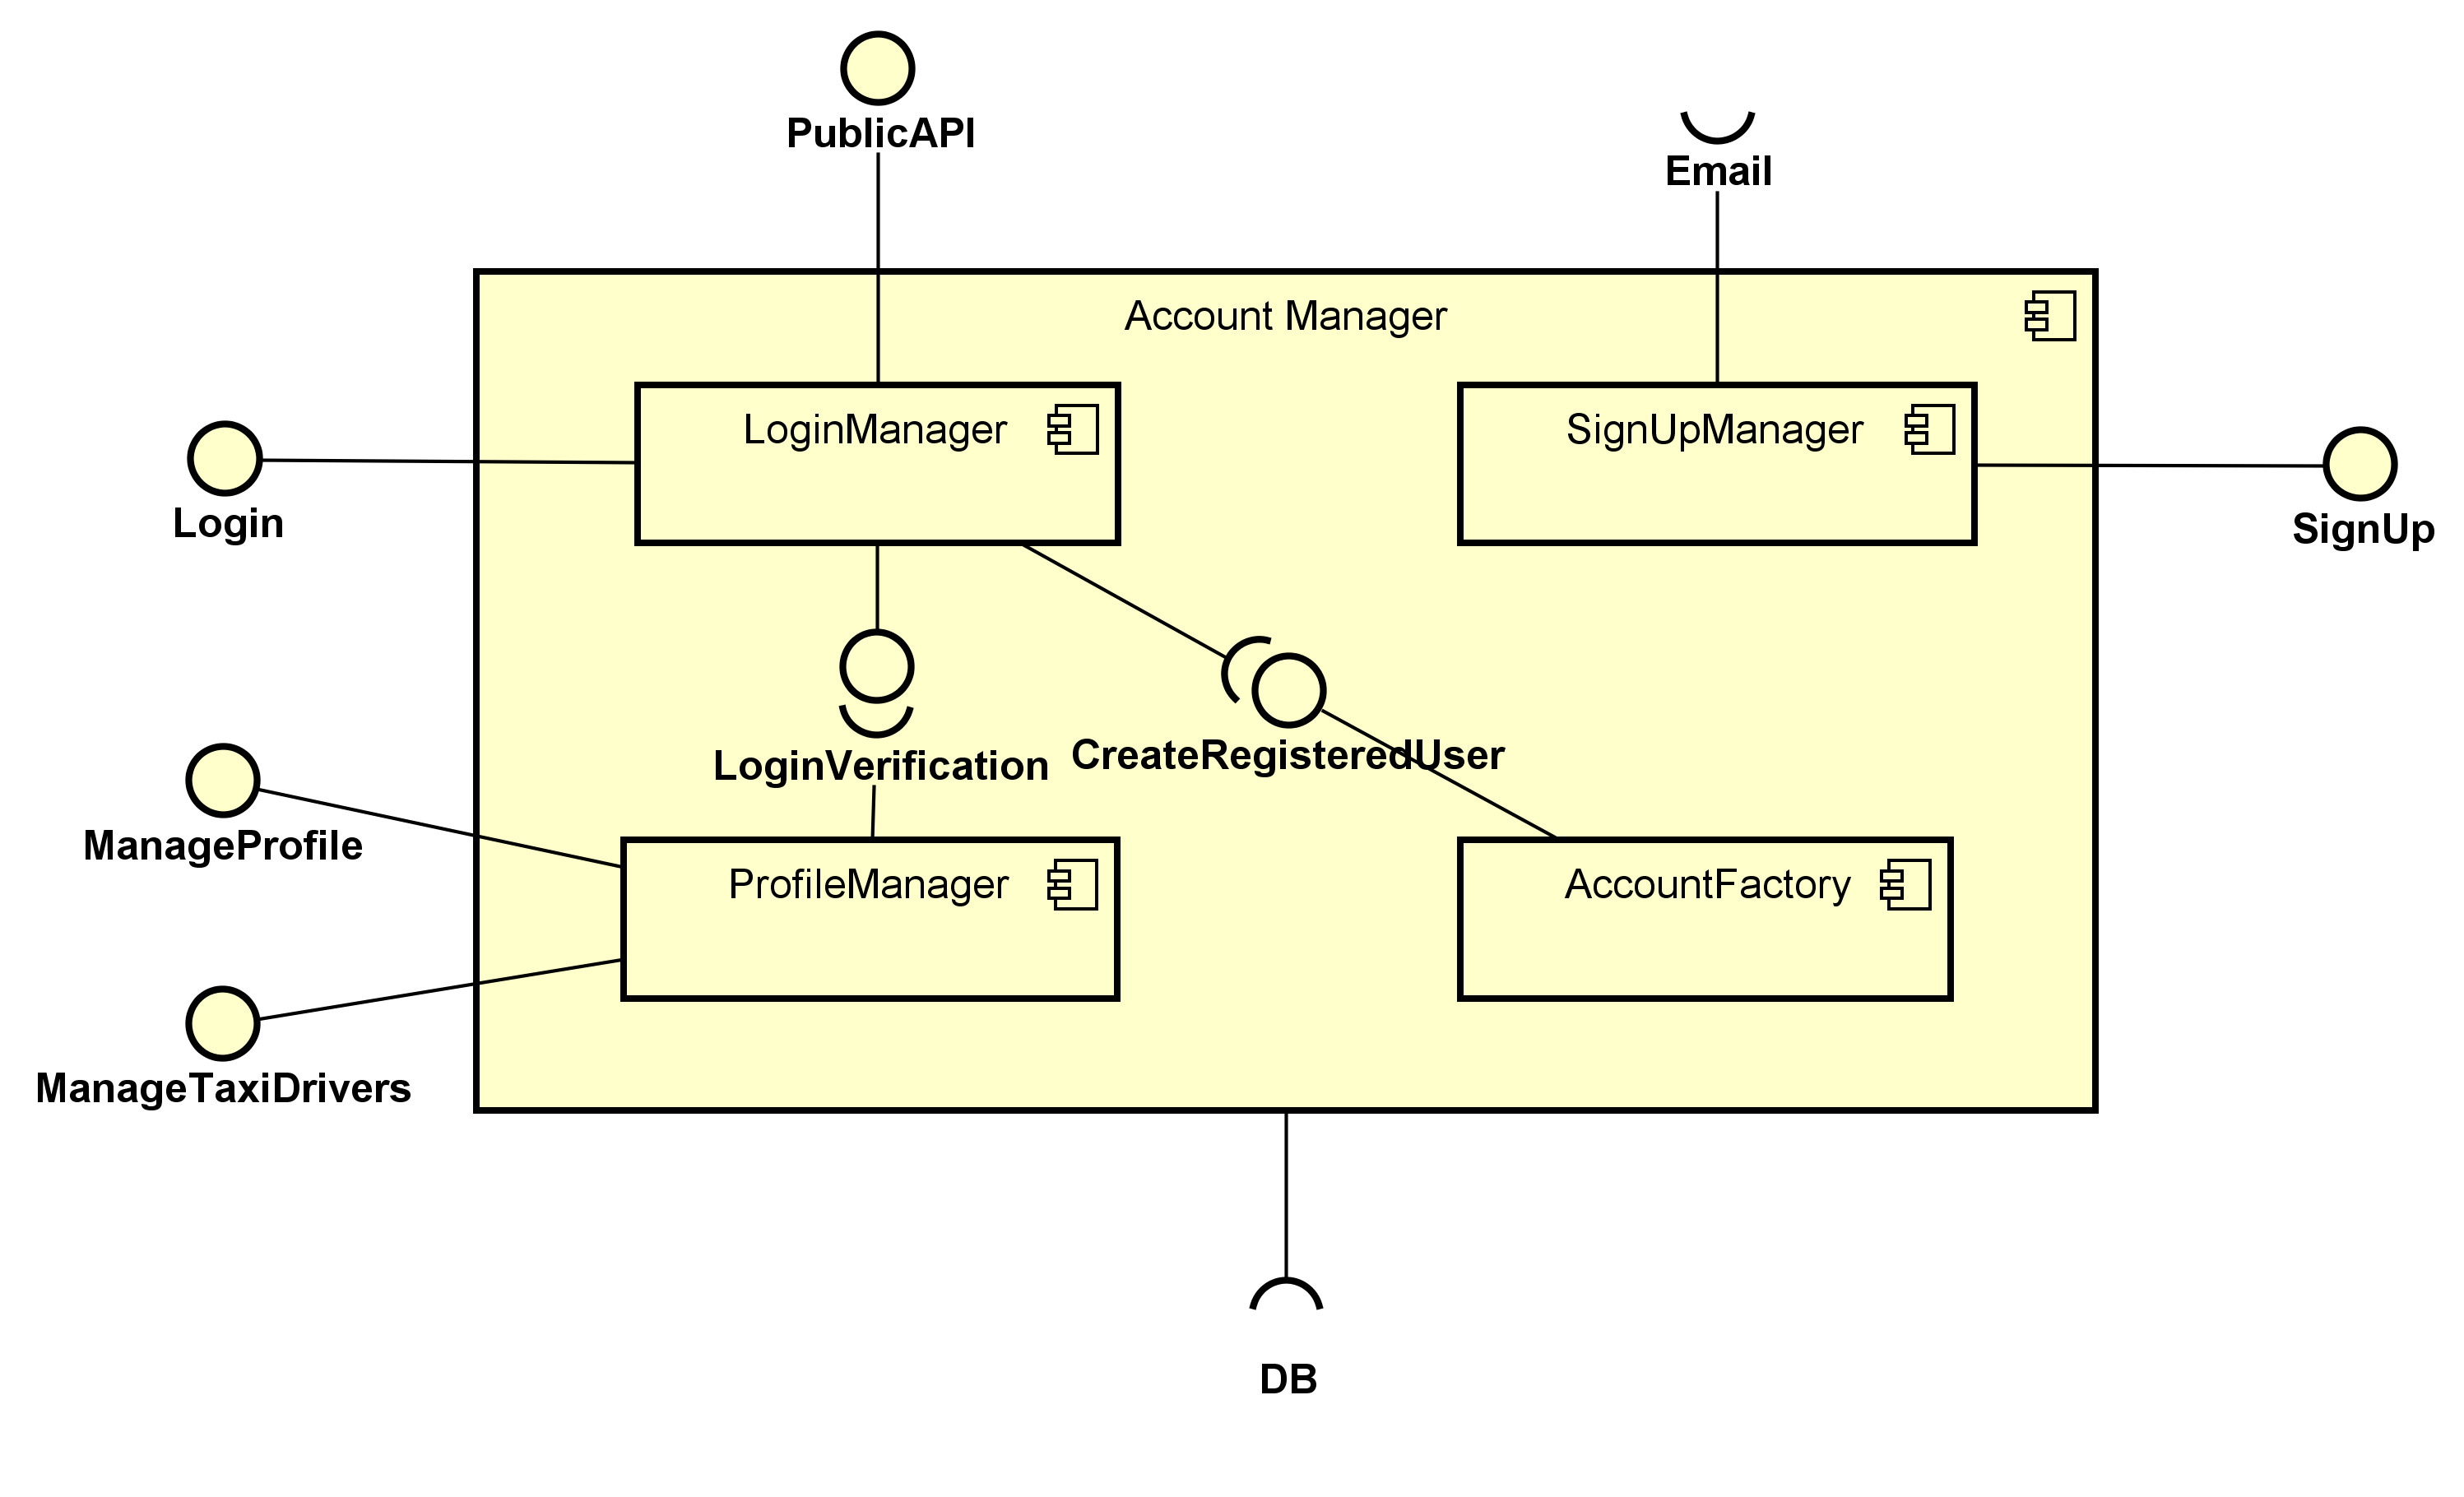
\includegraphics[keepaspectratio=true,scale=0.6]{Pictures/CVAccountManager}}
	\end{minipage} \linebreak
	\centerline{SignUpManager:}	
	\begin{center}
		\begin{tabular}{| l | p{9cm} |}\hline
			Definition & Component controlling the visitors' sign up.\\\hline
			Responsibilities & This component allows visitors to sign up into \mts{} and become registered users. It connects to the DB to store the credentials and requires and Email interface to verify the sign up procedure through a confirmation link sent via email.\\\hline
			Interaction & With the visitors, the DB and email service.\\\hline
			Interfaces offered & \begin{itemize}
				\item SignUp for Visitor
			\end{itemize}\\\hline
			Interfaces required & \begin{itemize}
				\item DB 
				\item External Email service
			\end{itemize}\\\hline
			Implementation & Static class\\\hline
		\end{tabular}
	\end{center}
	
	\pagebreak
	\centerline{LoginManager:}	
	\begin{center}
		\begin{tabular}{| l | p{9cm} |}\hline
			Definition & Component controlling the users' login.\\\hline
			Responsibilities & This component allows users to login into \mts{}. It is connected to the DB to verify the credentials and grants access to the ProfileManager. It offers the possibility to login to the service to third party apps.\\\hline
			Interaction & With all the users of the system, with the DB and external services (APIs).\\\hline
			Interfaces offered & \begin{itemize}
				\item Login for User
				\item LoginVerification for ProfileManager
				\item PublicAPI for external services
			\end{itemize}\\\hline
			Interfaces required & \begin{itemize}
				\item DB 
			\end{itemize}\\\hline
			Implementation & Static class\\\hline
		\end{tabular}
	\end{center}
	\bigskip
	\bigskip
	\centerline{ProfileManager:}
	\begin{center}
		\begin{tabular}{| l | p{9cm} |}\hline
			Definition & Component controlling the users' profile.\\\hline
			Responsibilities & This component allows users to edit their profile, for instance to change the password, credit card data, phone number, notifications type. It permits the Administrator to add or edit taxi drivers.\\\hline
			Interaction & With all the RegisteredUser of the system, with the DB and with the LoginManager component.\\\hline
			Interfaces offered & \begin{itemize}
				\item ManageProfile for RegisteredUser
				\item ManageTaxiDrivers for Administrator
			\end{itemize}\\\hline
			Interfaces required & \begin{itemize}
				\item DB
				\item LoginVerification for LoginManager
			\end{itemize}\\\hline
			Implementation & Multi instance: one for each user session (where session means the entire period of time in which the user is logged in)\\\hline
		\end{tabular}
	\end{center}
	
	\pagebreak
	\centerline{AccountFactory:}
	\begin{center}
		\begin{tabular}{| l | p{9cm} |}\hline
			Definition & Component which instantiates the users.\\\hline
			Responsibilities & This component is in charge of the creation of an instance for every logged in user. It is an example of ``Factory method'' pattern.\\\hline
			Interaction & With the LoginManager and the DB.\\\hline
			Interfaces offered & \begin{itemize}
				\item CreateRegisteredUser for LoginManager
			\end{itemize}\\\hline
			Interfaces required & \begin{itemize}
				\item DB
			\end{itemize}\\\hline
			Implementation & Factory method pattern\\\hline
		\end{tabular}
	\end{center}
			
	\pagebreak
	\subsubsection{Request Manager}
	\begin{minipage}{\linewidth}
		%		\vspace*{-0.35cm}
		\makebox[\linewidth]{
			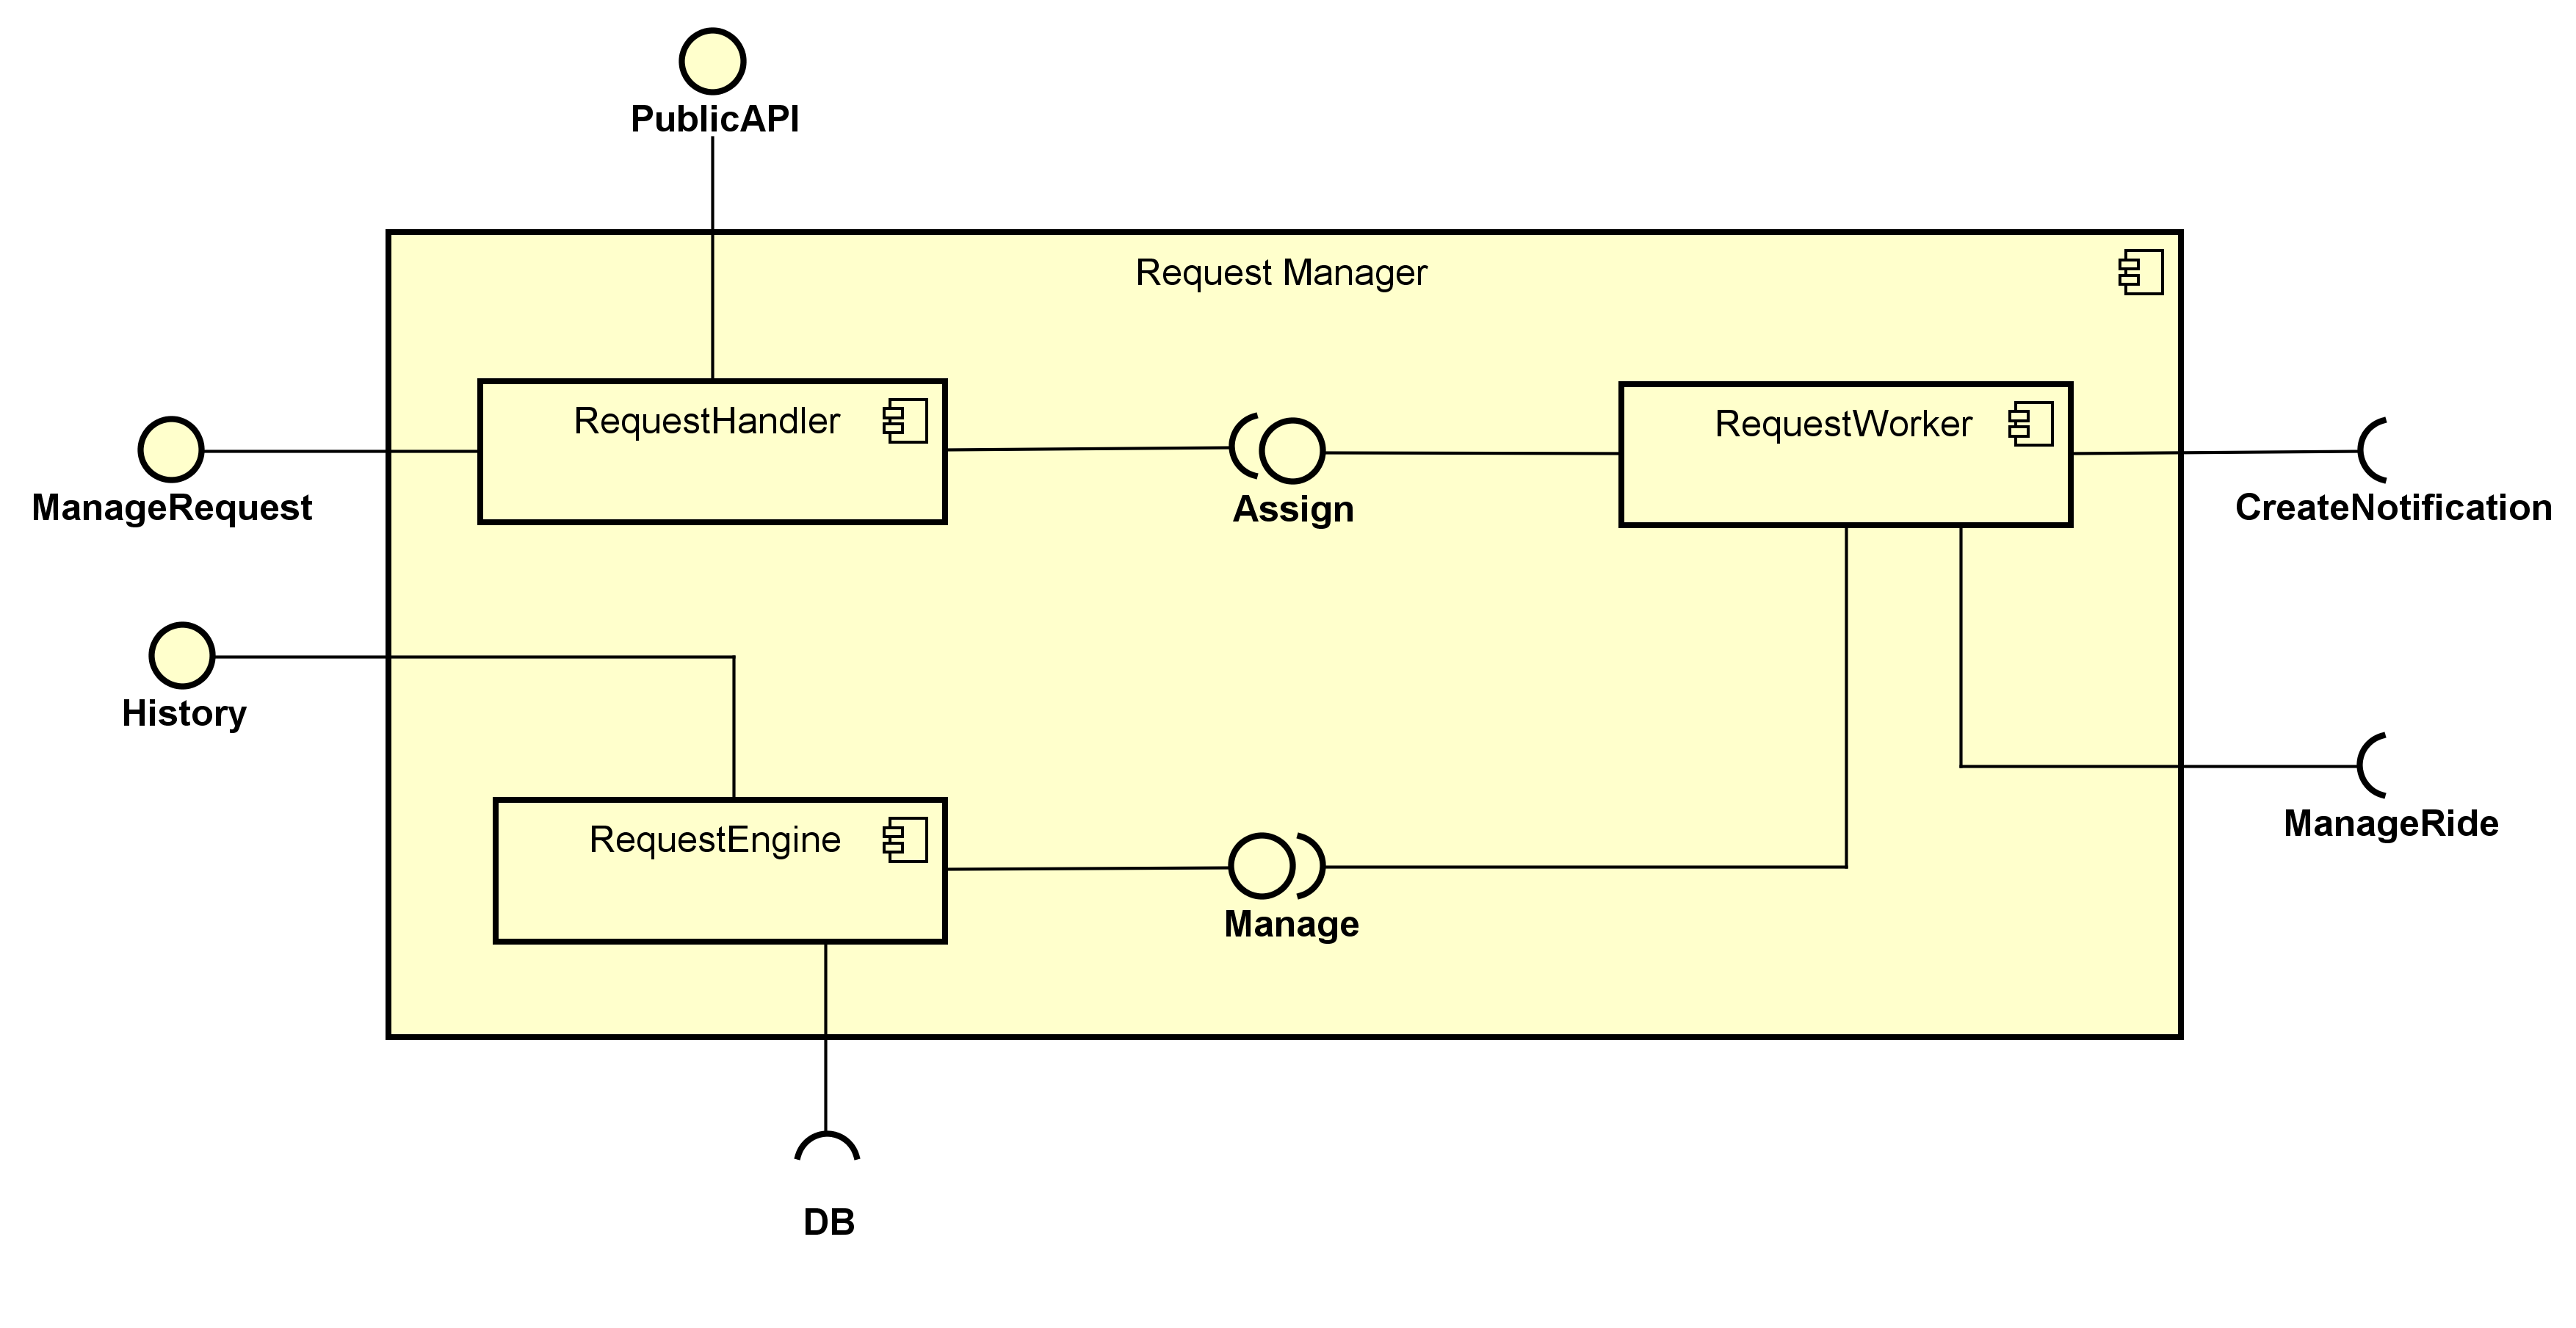
\includegraphics[keepaspectratio=true,scale=0.6]{Pictures/CVRequestManager}}
	\end{minipage} \linebreak
	\centerline{RequestHandler:}
	\begin{center}
		\begin{tabular}{| l | p{9cm} |}\hline
			Definition & Component receiving the passengers' requests.\\\hline
			Responsibilities & This component receives the requests or reservations of the clients and for each of them starts a ``worker'' that will handle them singularly. It also offers functions to enable the access of users from external services who can then send in requests.\\\hline
			Interaction & With all the Passengers from inside the system or external services and with the RequestWorker component to start a thread for every request.\\\hline
			Interfaces offered & \begin{itemize}
				\item ManageRequest for Passenger
				\item PublicAPI for external services
			\end{itemize}\\\hline
			Interfaces required & \begin{itemize}
				\item Assign for RequestWorker
			\end{itemize}\\\hline
			Implementation & Factory method pattern\\\hline
		\end{tabular}
	\end{center}
	
	\pagebreak
	\vspace*{-0.35cm}
	\centerline{RequestEngine:}
	\begin{center}
		\begin{tabular}{| l | p{9cm} |}\hline
			Definition & Component maintaining the history of the passengers' requests.\\\hline
			Responsibilities & This component keeps stored in the DB all the information of the past and active requests for every user who can browse his/her own history or modify current requests. Of course it accesses the DB.\\\hline
			Interaction & With all the Passengers, with the RequestWorker components to receive updates from every request and with the DB to store persistently the data.\\\hline
			Interfaces offered & \begin{itemize}
				\item History for Passenger
				\item Manage for RequestWorker
			\end{itemize}\\\hline
			Interfaces required & \begin{itemize}
				\item DB
			\end{itemize}\\\hline
			Implementation & Singleton\\\hline
		\end{tabular}
	\end{center}		
	
	\vspace*{0.35cm}
	\centerline{RequestWorker:}
	\begin{center}
		\begin{tabular}{| l | p{9cm} |}\hline
			Definition & Component managing individually the requests of the users.\\\hline
			Responsibilities & There is an instance of this component for every request generated by the users. It communicates updates of the request to the Notification manager. It is also connected to the RideManager to start the process of creation of the ride at the decided time.\\\hline
			Interaction & With the NotificationManager, with the RideManager, and with the RequestEngine to store the data about the requests in the DB.\\\hline
			Interfaces offered & \begin{itemize}
				\item Assign for RequestHandler
			\end{itemize}\\\hline
			Interfaces required & \begin{itemize}
				\item CreateNotification for NotificationManager
				\item ManageRide for RideManager
				\item Manage for RequestEngine
			\end{itemize}\\\hline
			Implementation & Multi instance: one for each request\\\hline
		\end{tabular}
	\end{center}	
	
	\subsubsection{Ride Manager}
	\begin{minipage}{\linewidth}
		%		\vspace*{-0.35cm}
		\makebox[\linewidth]{
			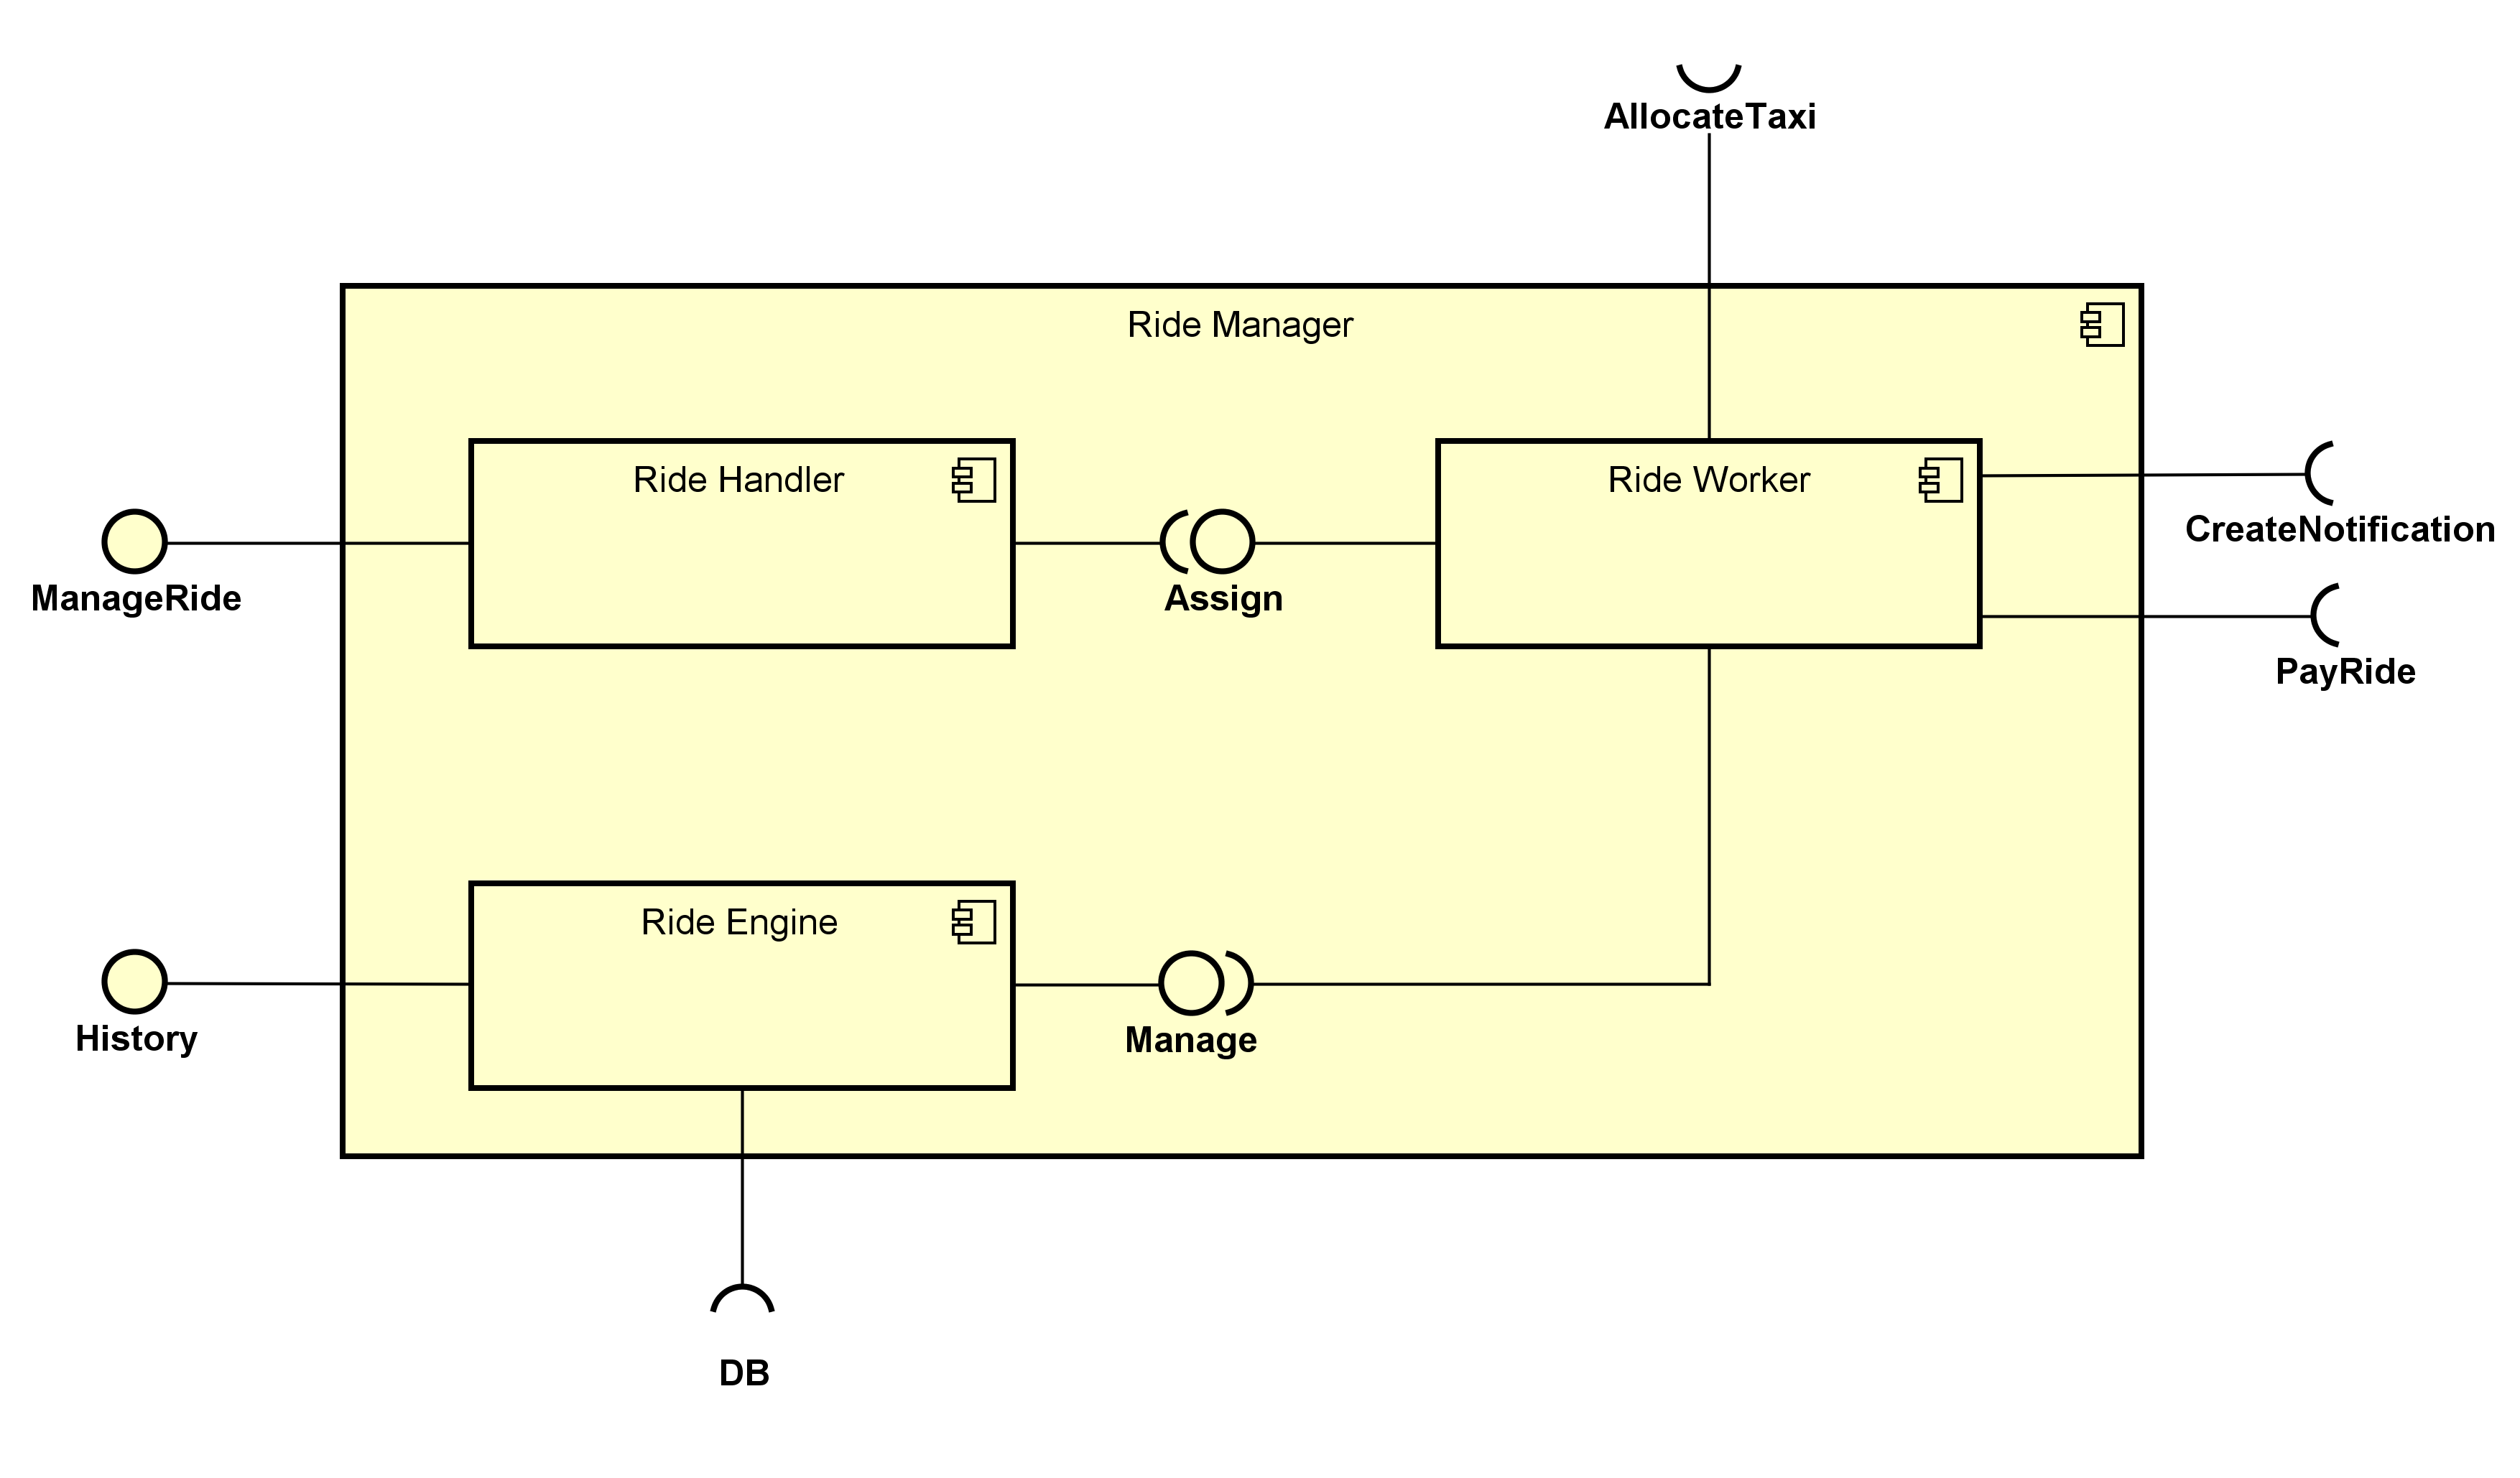
\includegraphics[keepaspectratio=true,scale=0.6]{Pictures/CVRideManager}}
	\end{minipage} \linebreak
	\centerline{RideHandler:}
	\begin{center}
		\begin{tabular}{| l | p{9cm} |}\hline
			Definition & Component that creates the rides.\\\hline
			Responsibilities & This component creates the rides from the corresponding requests at the decided time (10 minutes before the meeting time for the reservations), for this reason it communicates with the RequestManager. Later it assigns every generated ride to an instance of RideWorker which will handle it singularly.\\\hline
			Interaction & With the RequestManager and with the RideWorker component to start a thread for every ride.\\\hline
			Interfaces offered & \begin{itemize}
				\item ManageRide for RequestManager
			\end{itemize}\\\hline
			Interfaces required & \begin{itemize}
				\item Assign for RideWorker
			\end{itemize}\\\hline
			Implementation & Factory method pattern\\\hline
		\end{tabular}
	\end{center}
	
	\pagebreak
	\vspace*{-0.35cm}
	\centerline{RideEngine:}
	\begin{center}
		\begin{tabular}{| l | p{9cm} |}\hline
			Definition & Component maintaining the history of the drivers' rides.\\\hline
			Responsibilities & This component keeps stored in the DB all the information of the past and active rides for every user who can browse his/her own history or modify current rides. Of course it accesses the DB.\\\hline
			Interaction & With all the drivers, with the RideWorker components to receive updates from every ride and with the DB to store persistently the data.\\\hline
			Interfaces offered & \begin{itemize}
				\item History for TaxiDriver
				\item Manage for RideWorker
			\end{itemize}\\\hline
			Interfaces required & \begin{itemize}
				\item DB
			\end{itemize}\\\hline
			Implementation & Singleton\\\hline
		\end{tabular}
	\end{center}		
	
	\pagebreak
	\centerline{RideWorker:}
	\begin{center}
		\begin{tabular}{| l | p{9cm} |}\hline
			Definition & Component managing individually the rides of the users.\\\hline
			Responsibilities & There is an instance of this component for every ride generated by the system. It communicates updates of the ride to the NotificationManager to warn involved passengers and the driver. It is also connected to the ZoneManager to allocate a taxi once the ride is created and with the PaymentManager to collect money when the passenger needs to pay a fine or the taxi fare. It is connected with the RideEngine to store the data of the ride in the DB.\\\hline
			Interaction & With the NotificationManager, with the ZoneManager, with the RideEngine and with the PaymentManager.\\\hline
			Interfaces offered & \begin{itemize}
				\item Assign for RideHandler
			\end{itemize}\\\hline
			Interfaces required & \begin{itemize}
				\item CreateNotification for NotificationManager
				\item AllocateTaxi for ZoneManager
				\item PayRide for PaymentManager
			\end{itemize}\\\hline
			Implementation & Multi instance: one for each ride\\\hline
		\end{tabular}
	\end{center}	
	
	\pagebreak
	\subsubsection{Notification Manager}
	\begin{minipage}{\linewidth}
		%		\vspace*{-0.35cm}
		\makebox[\linewidth]{
			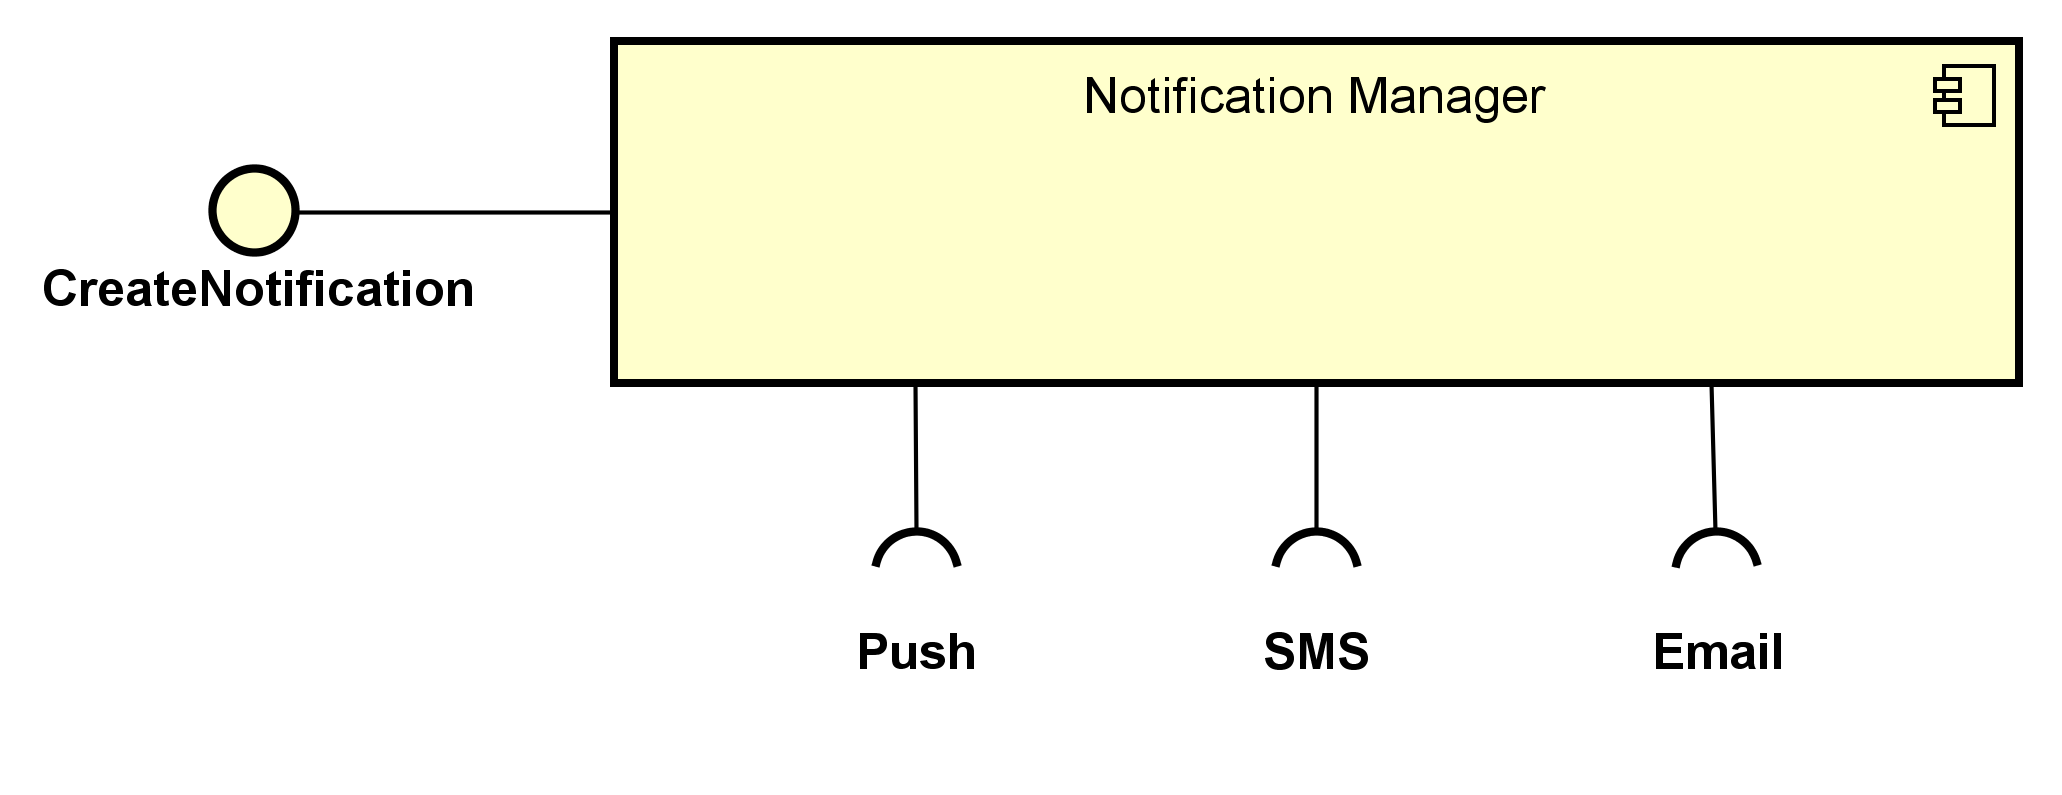
\includegraphics[keepaspectratio=true,scale=0.65]{Pictures/CVNotificationManager}}
	\end{minipage} \linebreak
	\centerline{NotificationManager:}
	\begin{center}
		\begin{tabular}{| l | p{9cm} |}\hline
			Definition & Component controlling the notifications sent to the users.\\\hline
			Responsibilities & This component is able to receive a message to be sent to some users with the specification of the mean of communication to be used. For this reason it is connected to the external services managing the dispatching of SMS, Emails and in-app push notifications.\\\hline
			Interaction & With the RequestManager and RideManager to send updates about the request/rides to the passengers involved, with the ZoneManager to send updates to taxi drivers, and with the external services of SMS and Email.\\\hline
			Interfaces offered & \begin{itemize}
				\item CreateNotification for RideManager, RequestManager and ZoneManager
			\end{itemize}\\\hline
			Interfaces required & \begin{itemize}
				\item Push for external services
				\item SMS for external services
				\item Email for external services
			\end{itemize}\\\hline
			Implementation & Static class\\\hline
		\end{tabular}
	\end{center}	
		
	\pagebreak
	\subsubsection{Taxi Manager}
	\begin{minipage}{\linewidth}
		%		\vspace*{-0.35cm}
		\makebox[\linewidth]{
			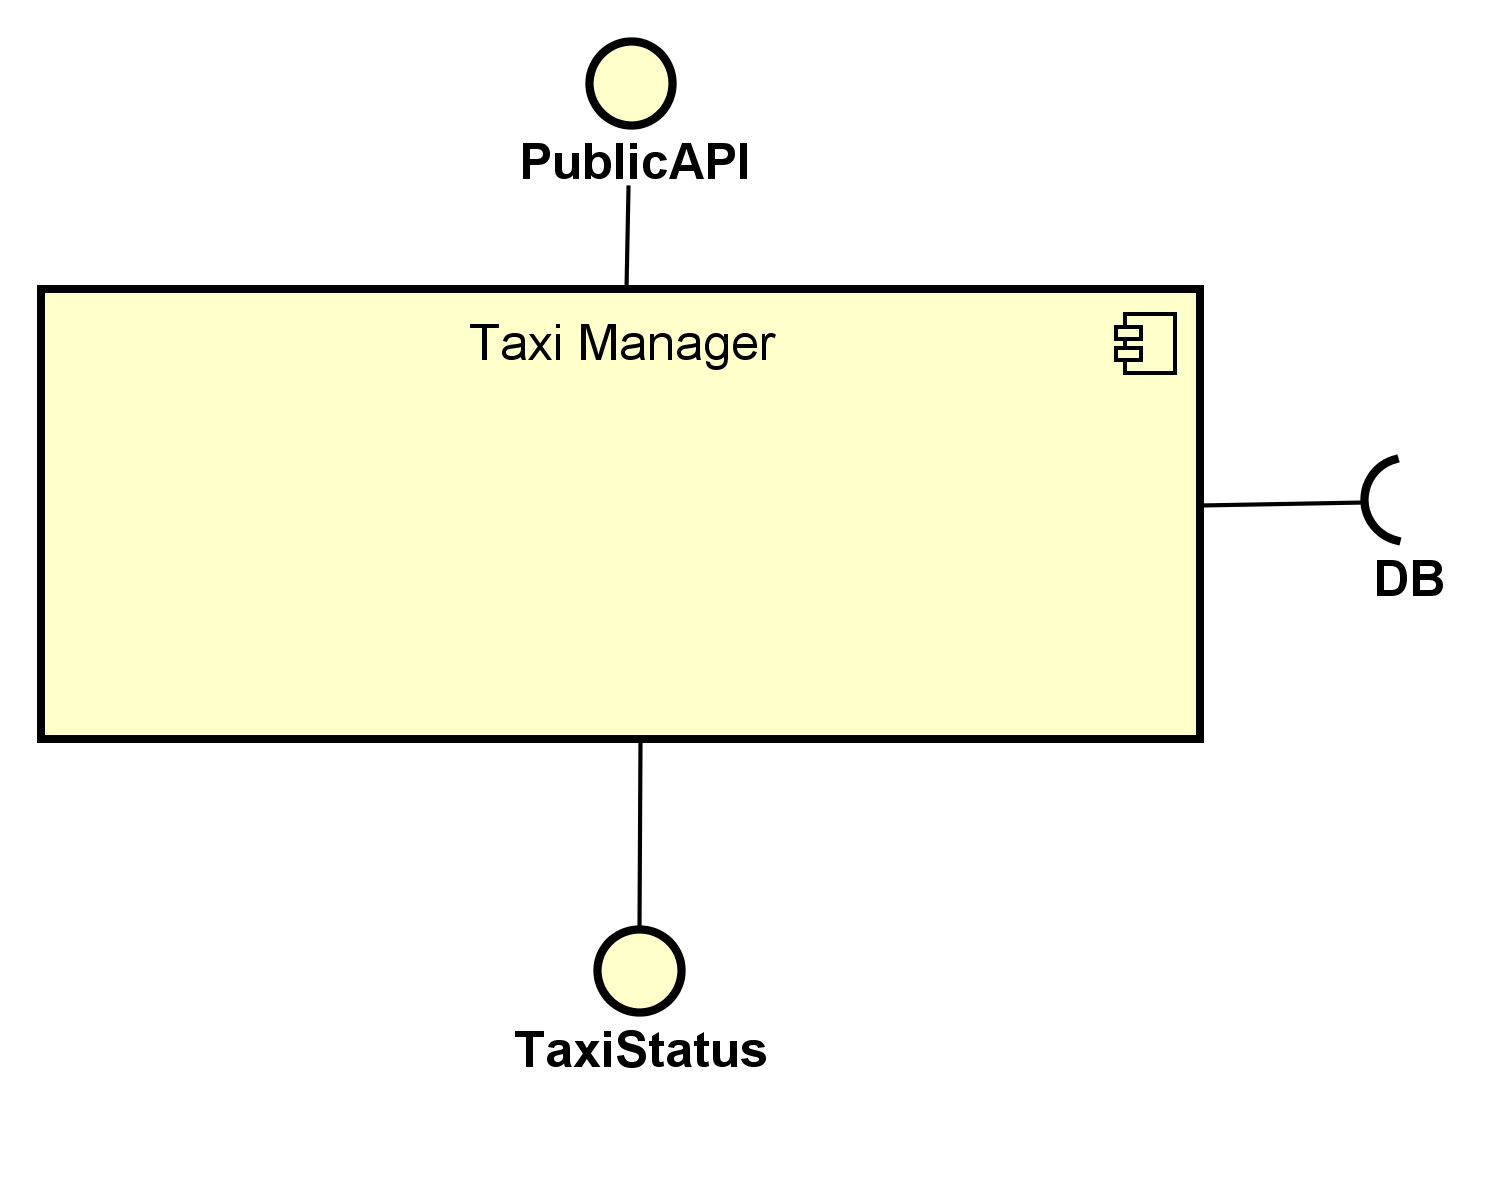
\includegraphics[keepaspectratio=true,scale=0.6]{Pictures/CVTaxiManager}}
	\end{minipage} \linebreak
	\centerline{TaxiManager:}
	\begin{center}
		\begin{tabular}{| l | p{9cm} |}\hline
			Definition & Controller of the current situation of every taxi.\\\hline
			Responsibilities & This component keeps track of all the information about the whole taxi fleet. It can retrieve the position of taxis as well as their availability status and send these to the ZoneManager which uses them to control the queues and assign jobs. Thanks to the information about the location of every taxi, an external service can retrieve the current situation of the taxis spread across the city and possibly show them on a map.\\\hline
			Interaction & With the ZoneManager to make available information about taxis, with the DB to store the data and with external services to make these same information available outside the system.\\\hline
			Interfaces offered & \begin{itemize}
				\item TaxiStatus for ZoneManager
				\item PublicAPI for external services
			\end{itemize}\\\hline
			Interfaces required & \begin{itemize}
				\item DB
			\end{itemize}\\\hline
			Implementation & Singleton pattern\\\hline
		\end{tabular}
	\end{center}	
	
	\pagebreak
	\subsubsection{Zone Manager}
	\begin{minipage}{\linewidth}
		%		\vspace*{-0.35cm}
		\makebox[\linewidth]{
			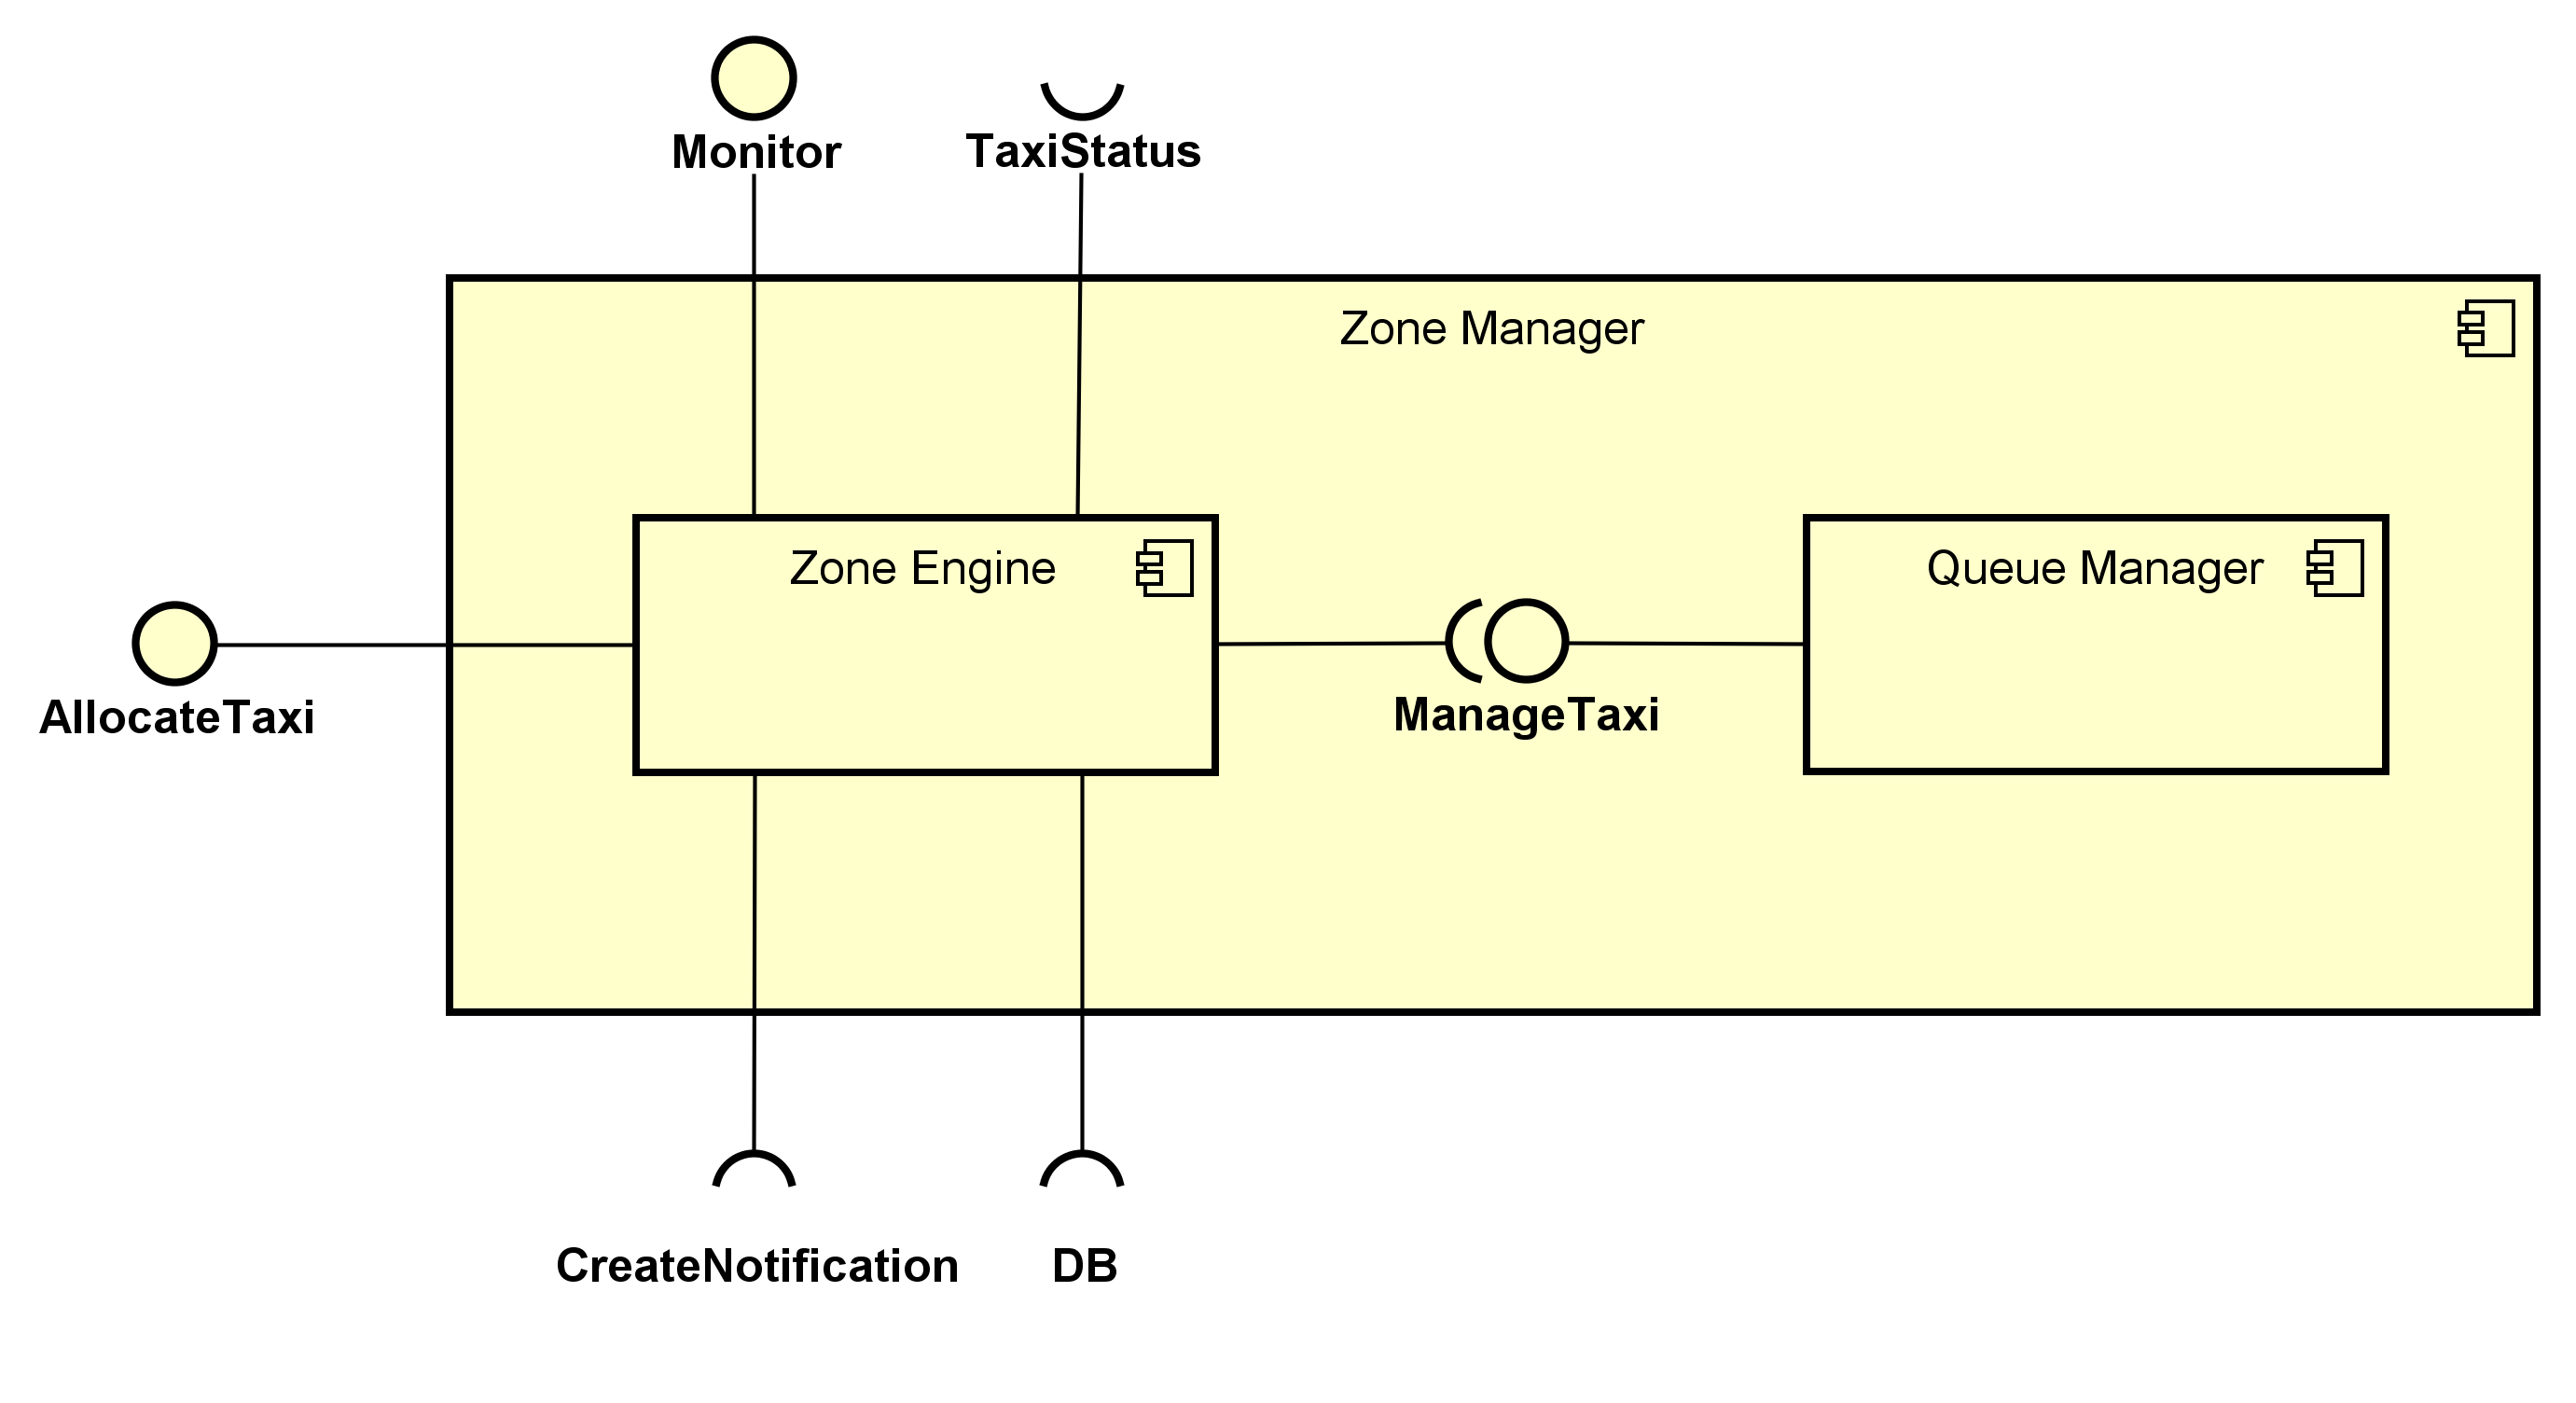
\includegraphics[keepaspectratio=true,scale=0.55]{Pictures/CVZoneManager}}
	\end{minipage}	\linebreak
	
	\centerline{QueueManager:}
	\begin{center}
		\begin{tabular}{| l | p{9cm} |}\hline
			Definition & Component controlling the queue of taxis in a single zone of the city.\\\hline
			Responsibilities & This component runs the algorithm to assign the jobs to its taxis and keeps the management of its queue fair. It receives the tasks to carry out from the ZoneEngine which only selects the correct zone.\\\hline
			Interaction & With the ZoneEngine.\\\hline
			Interfaces offered & \begin{itemize}
				\item ManageTaxi for ZoneEngine
			\end{itemize}\\\hline
			Implementation & Multi instance: one instance for each queue\\\hline
		\end{tabular}
	\end{center}
		
	\pagebreak
	\centerline{ZoneEngine:}
	\begin{center}
		\begin{tabular}{| l | p{9cm} |}\hline
			Definition & Component controlling the overall management of the city zones.\\\hline
			Responsibilities & This component is the manager of all the single queues, for this reason it is connected to the \textit{n} QueueManagers, where \textit{n} is the number of zones in the city. It is in charge of forwarding the requests of jobs/taxi assignation to the correct QueueManager. Being an overall summary of the current situation of the system it is connected with the Administrator who can monitor the real-time status of the service. All the data about the zones are stored in the DB. ZoneManager is called when RideManager needs to assign a driver to a specific ride, and the assignation is carried out with the cooperation of the TaxiManager which provides the availability status and position of every taxi. Once the assignation has been successfully completed ZoneManager notifies the driver through the NotificationManager.\\\hline
			Interaction & With the Administrator, TaxiManager, RideManager, NotificationManager and QueueManagers.\\\hline
			Interfaces offered & \begin{itemize}
				\item Monitor for Administrator
				\item AllocateTaxi for RideManager
			\end{itemize}\\\hline
			Interfaces required & \begin{itemize}
				\item TaxiStatus for TaxiManager
				\item CreateNotification for NotificationManager
				\item DB
			\end{itemize}\\\hline
			Implementation & Singleton\\\hline
		\end{tabular}
	\end{center}
	

	\pagebreak
	\subsubsection{Payment Manager}
	\begin{minipage}{\linewidth}
		%		\vspace*{-0.35cm}
		\makebox[\linewidth]{
			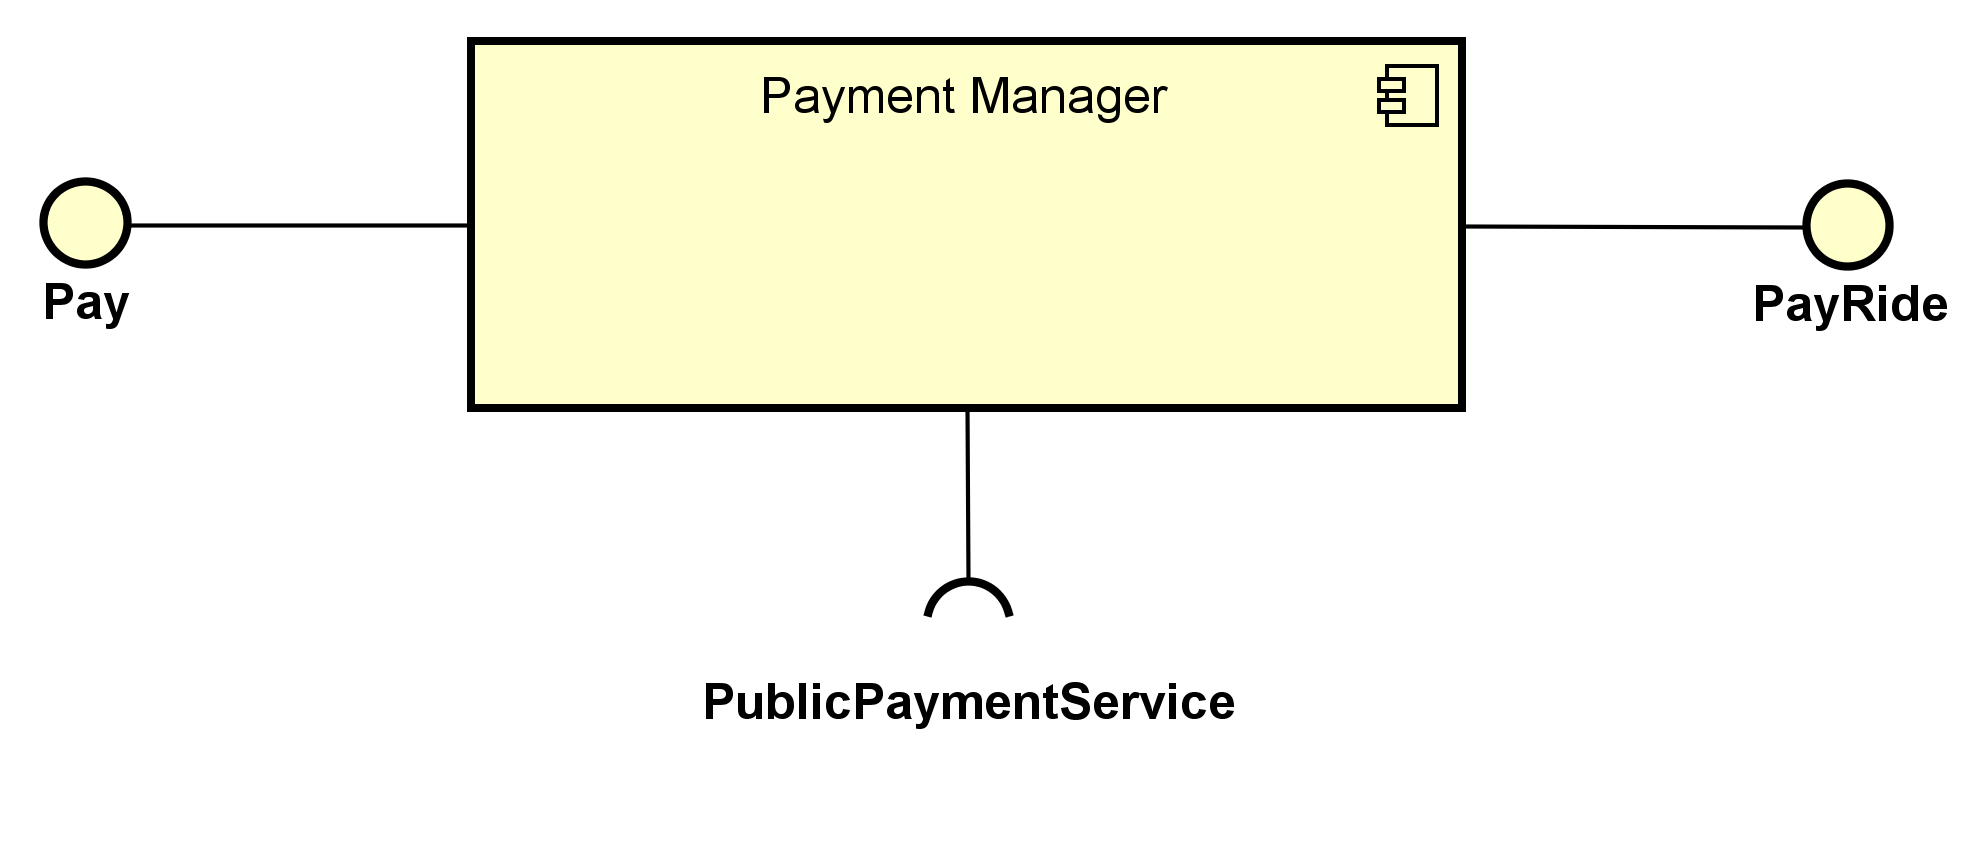
\includegraphics[keepaspectratio=true,scale=0.6]{Pictures/CVPaymentManager}}
	\end{minipage} \linebreak
	\centerline{PaymentManager:}
	\begin{center}
		\begin{tabular}{| l | p{9cm} |}\hline
			Definition & Component controlling the payment process\\\hline
			Responsibilities & This component is in charge of computing the amount of money (fine or fare) owed by each passenger (if the ride is shared). It interacts with the RideManager to receive information about the ride and with the Passenger to collect the money. It uses an interface to process the payment with external services.\\\hline
			Interaction & With all the Passengers of the system, with the RideManager and with external services.\\\hline
			Interfaces offered & \begin{itemize}
				\item Pay for Passenger
				\item PayRide for RideManager
			\end{itemize}\\\hline
			Interfaces required & \begin{itemize}
				\item PublicPaymentService for communication with external payment services.
			\end{itemize}\\\hline
			Implementation & Static class\\\hline
		\end{tabular}
	\end{center}

	\pagebreak
	\subsection{Deployment view}
	The schema below represents the diagram that models the physical deployment of the system with its main nodes.\\
	\begin{minipage}{\linewidth}
		%		\vspace*{-0.35cm}
		\makebox[\linewidth]{
			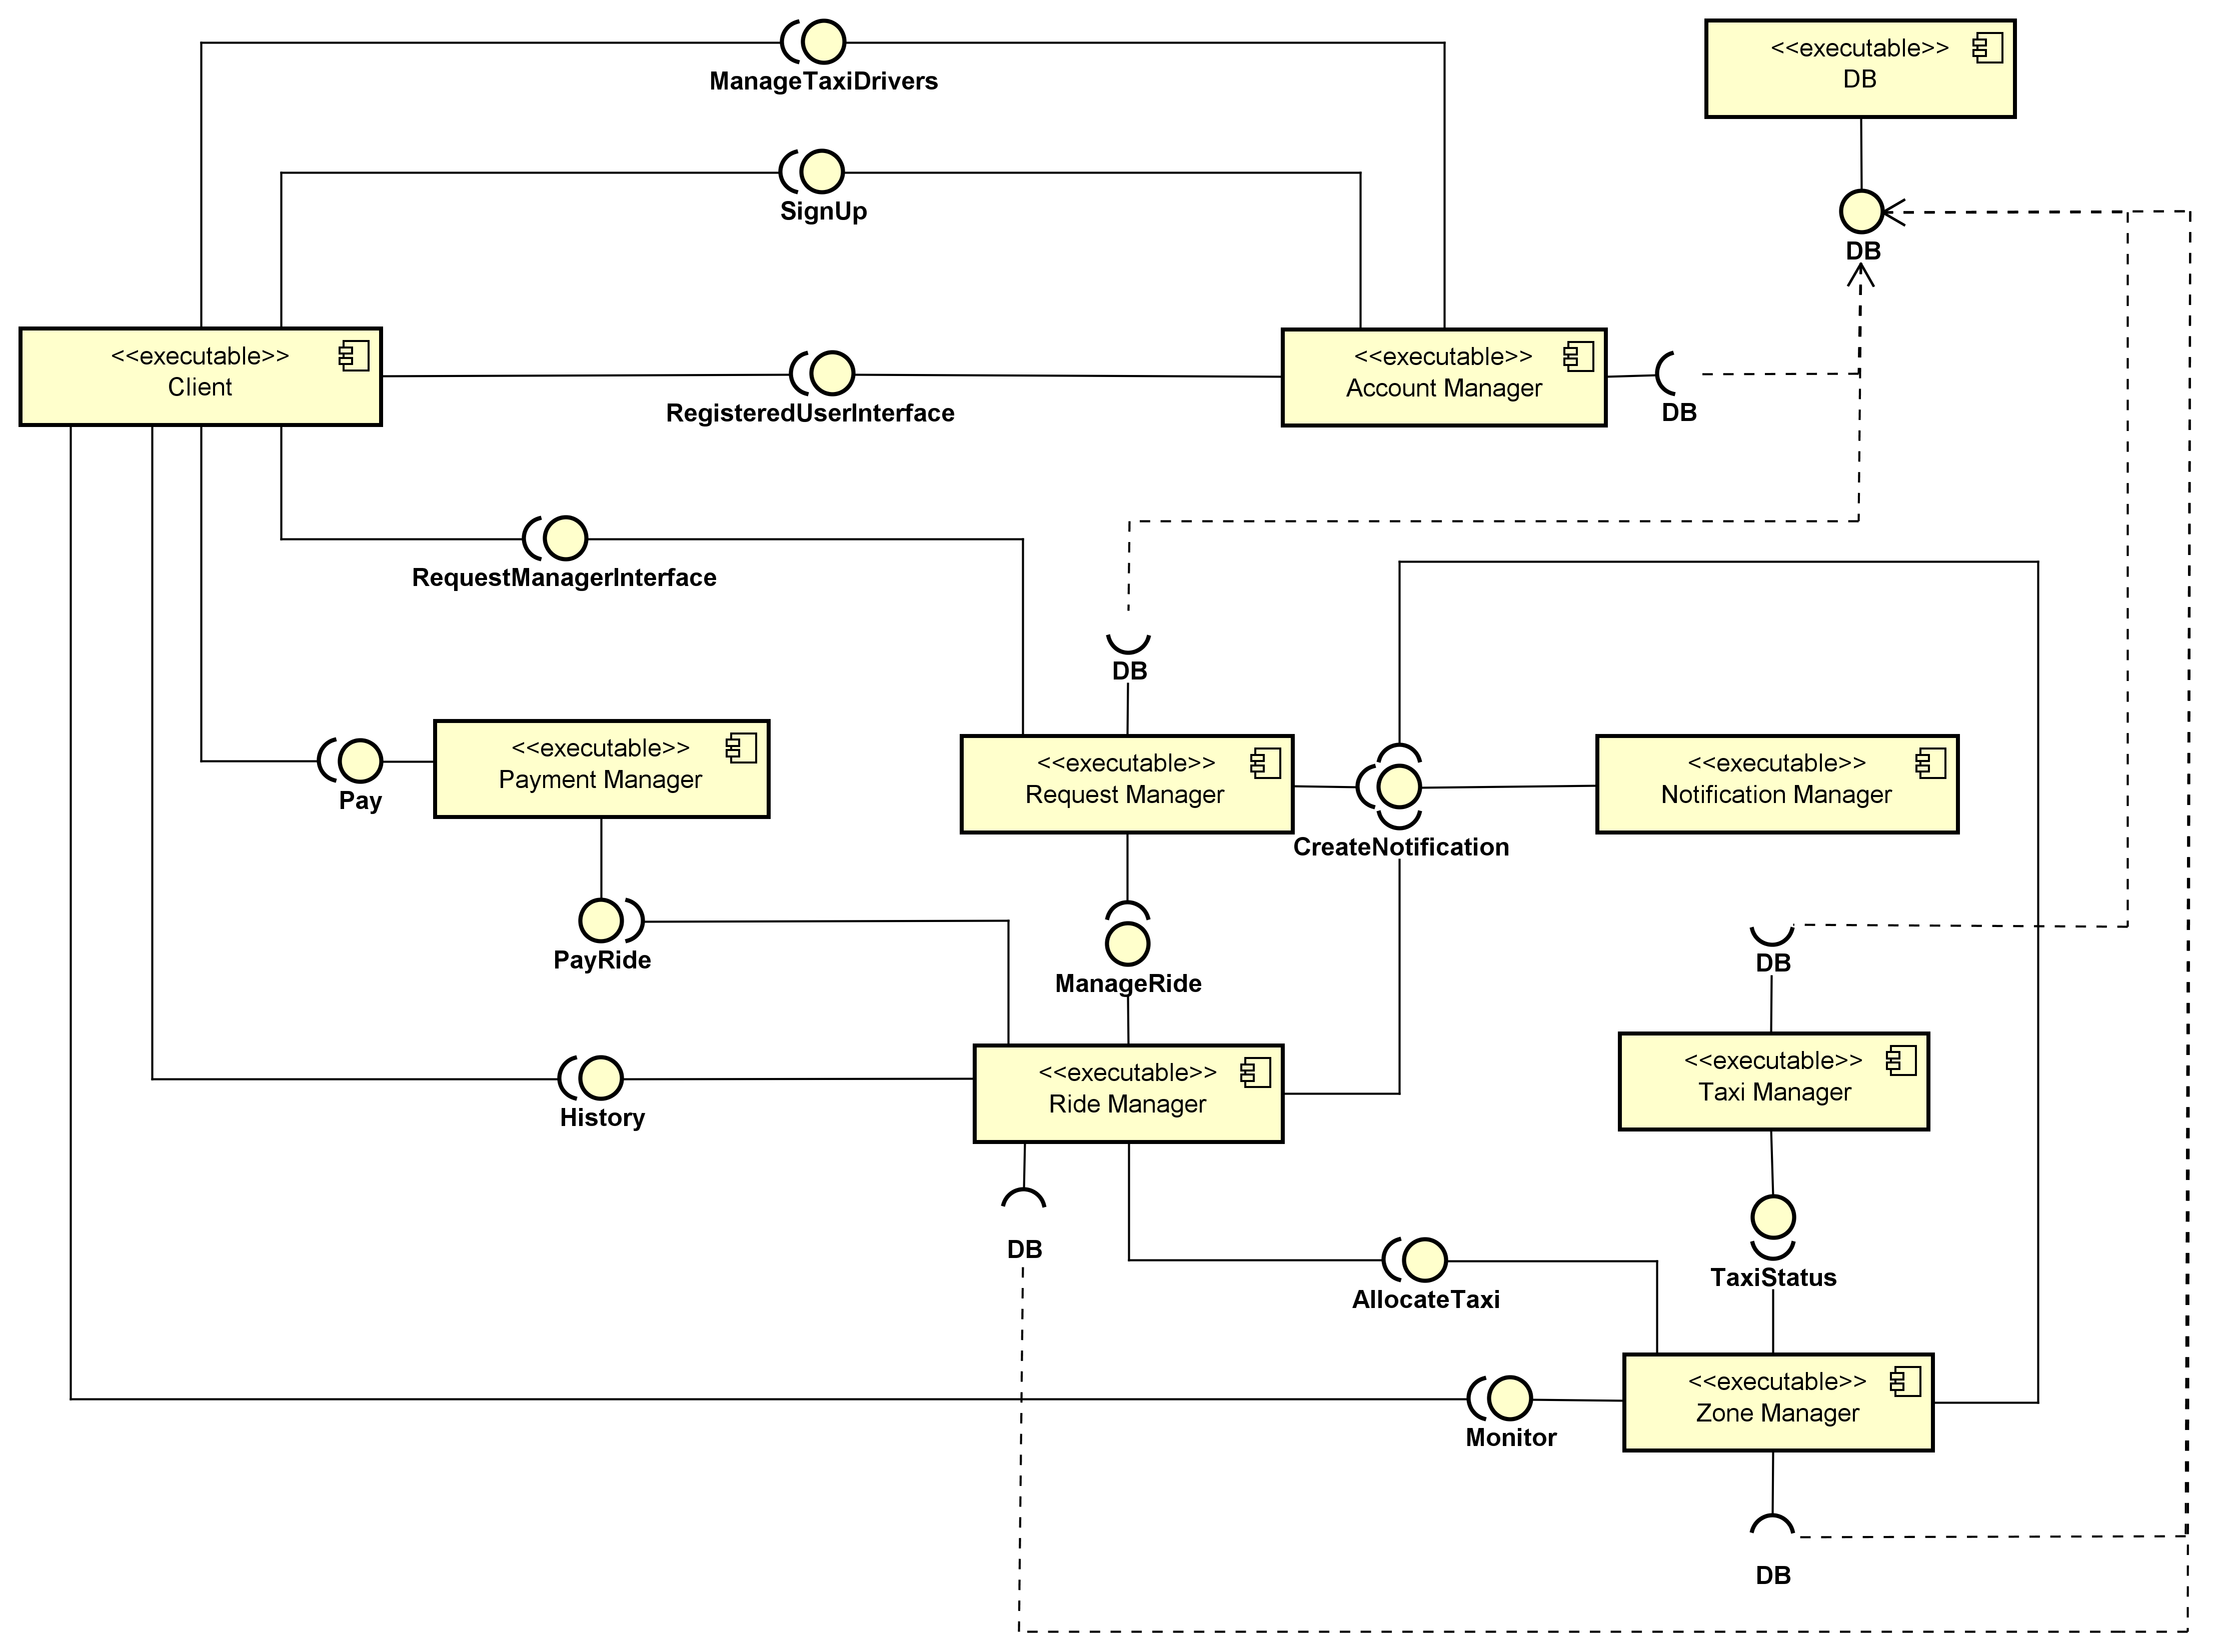
\includegraphics[keepaspectratio=true,scale=0.5]{Pictures/DeploymentView}}
	\end{minipage} \\

	\vspace*{+0.35cm}
	The diagram above shows which hardware components (``nodes'', boxes in the figure) exist in \mts{}:  the web server (``Client'' in the figure) that processes and delivers web pages to clients, an application server (all the ``Managers'' in the figure), a database server (``DB'' in the figure), and which software components run on each node (e.g., web application, database), and how the different pieces are connected.
	
	\pagebreak
	\subsection{Runtime view}
	\subsubsection{Runtime units}
	The schema below describes the behavior and interaction of the system's building blocks as runtime elements.\\
	\begin{minipage}{\linewidth}
		%		\vspace*{-0.35cm}
		\makebox[\linewidth]{
			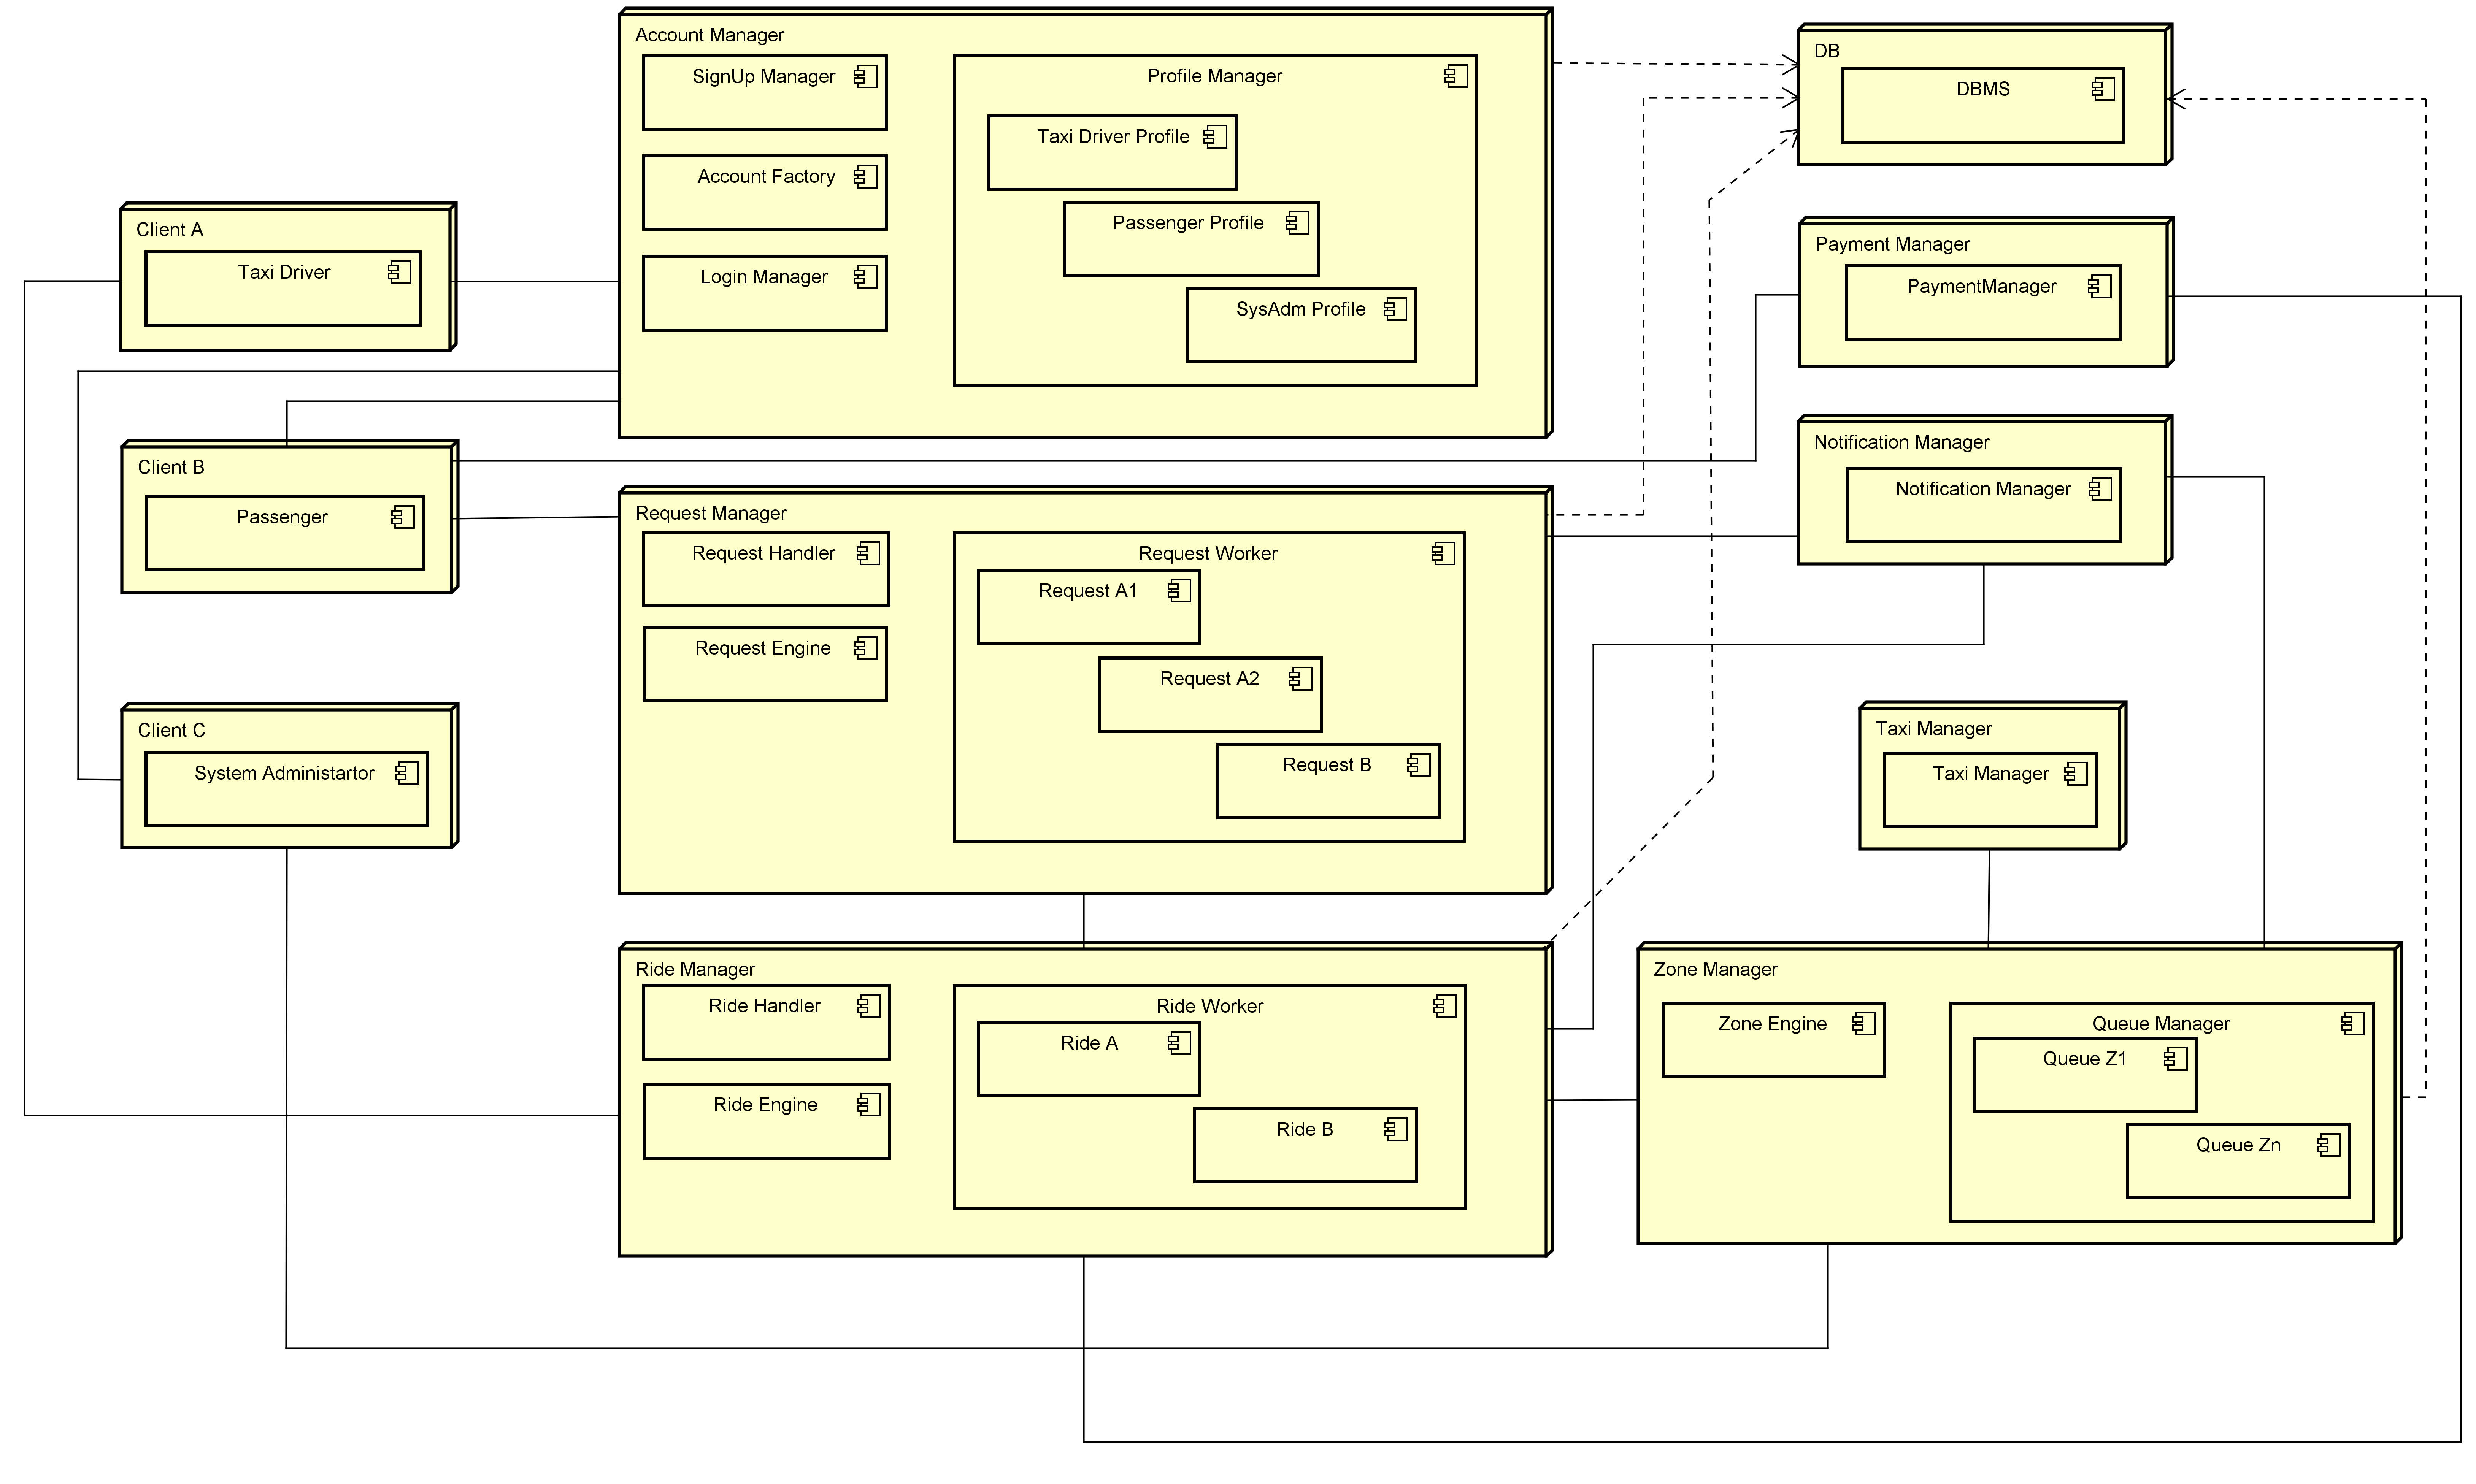
\includegraphics[keepaspectratio=true,scale=0.35]{Pictures/RuntimeView}}
	\end{minipage}
	The diagram clarifies which are the elements that at runtime exist possibly as multiple instances (on multiple threads) such as ProfileManager (one for each logged in user), RequestWorker (one for each request), RideWorker (one for each active ride), QueueManager (one for each zone of the city) and which are the components running on single processes.
	
	\pagebreak
	\subsubsection{Sequence diagrams}
	Below are presented some meaningful sequence diagrams that show the interaction between components at runtime.
	\paragraph{Login} \mbox{}\\ %mbox is to break the line after the title of the paragraph!
	Below is represented what happens when a registered user logins.\smallskip \\
		\begin{minipage}{\linewidth}
			%		\vspace*{-0.35cm}
			\makebox[\linewidth]{
				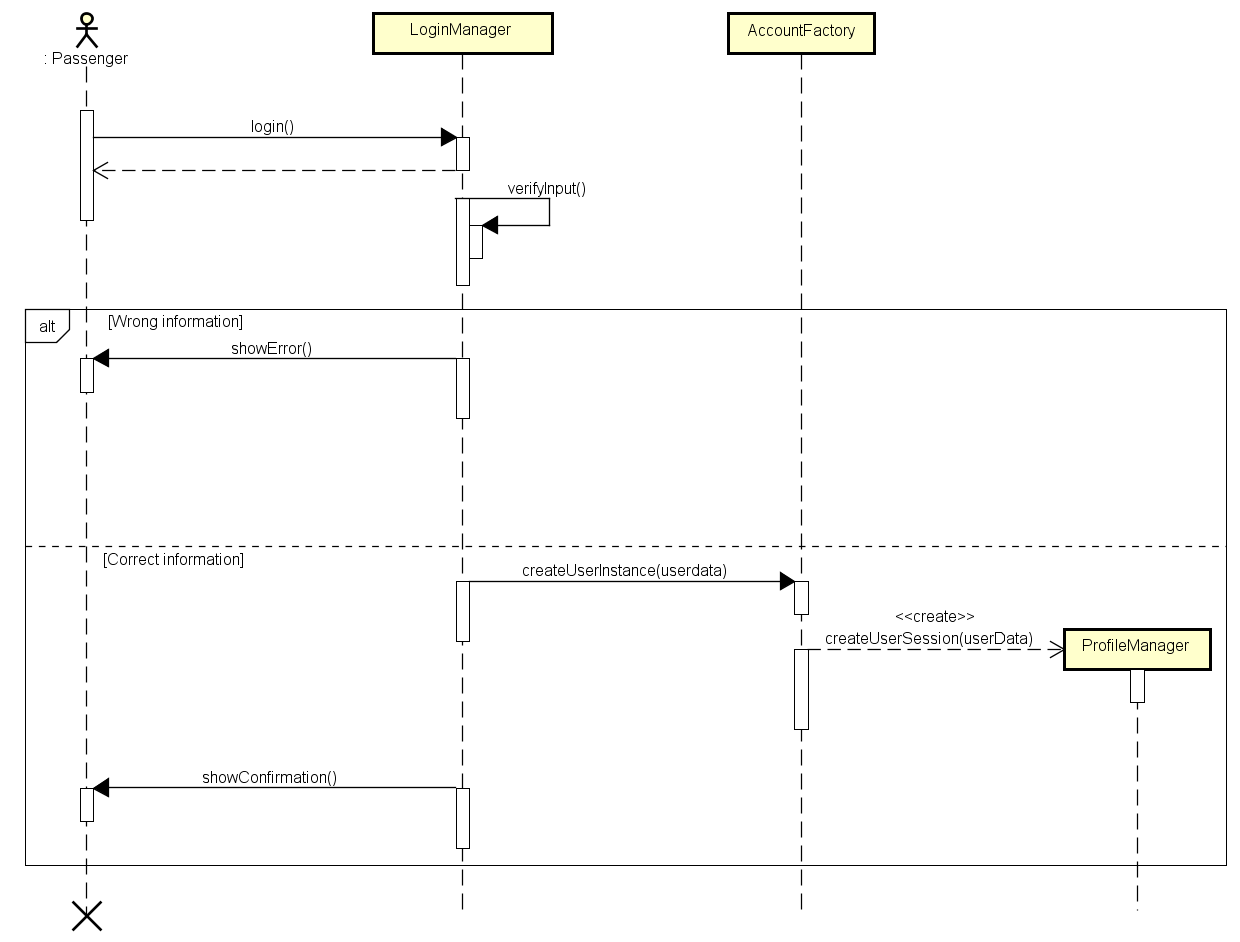
\includegraphics[keepaspectratio=true,scale=0.53]{Pictures/SDLogin}}
		\end{minipage}
		
	\pagebreak	
	\paragraph{Taxi request} \mbox{}\\
	Below is represented the interaction between components when an user asks for a taxi.\\	
		\begin{minipage}{\linewidth}
			%		\vspace*{-0.35cm}
			\makebox[\linewidth]{
				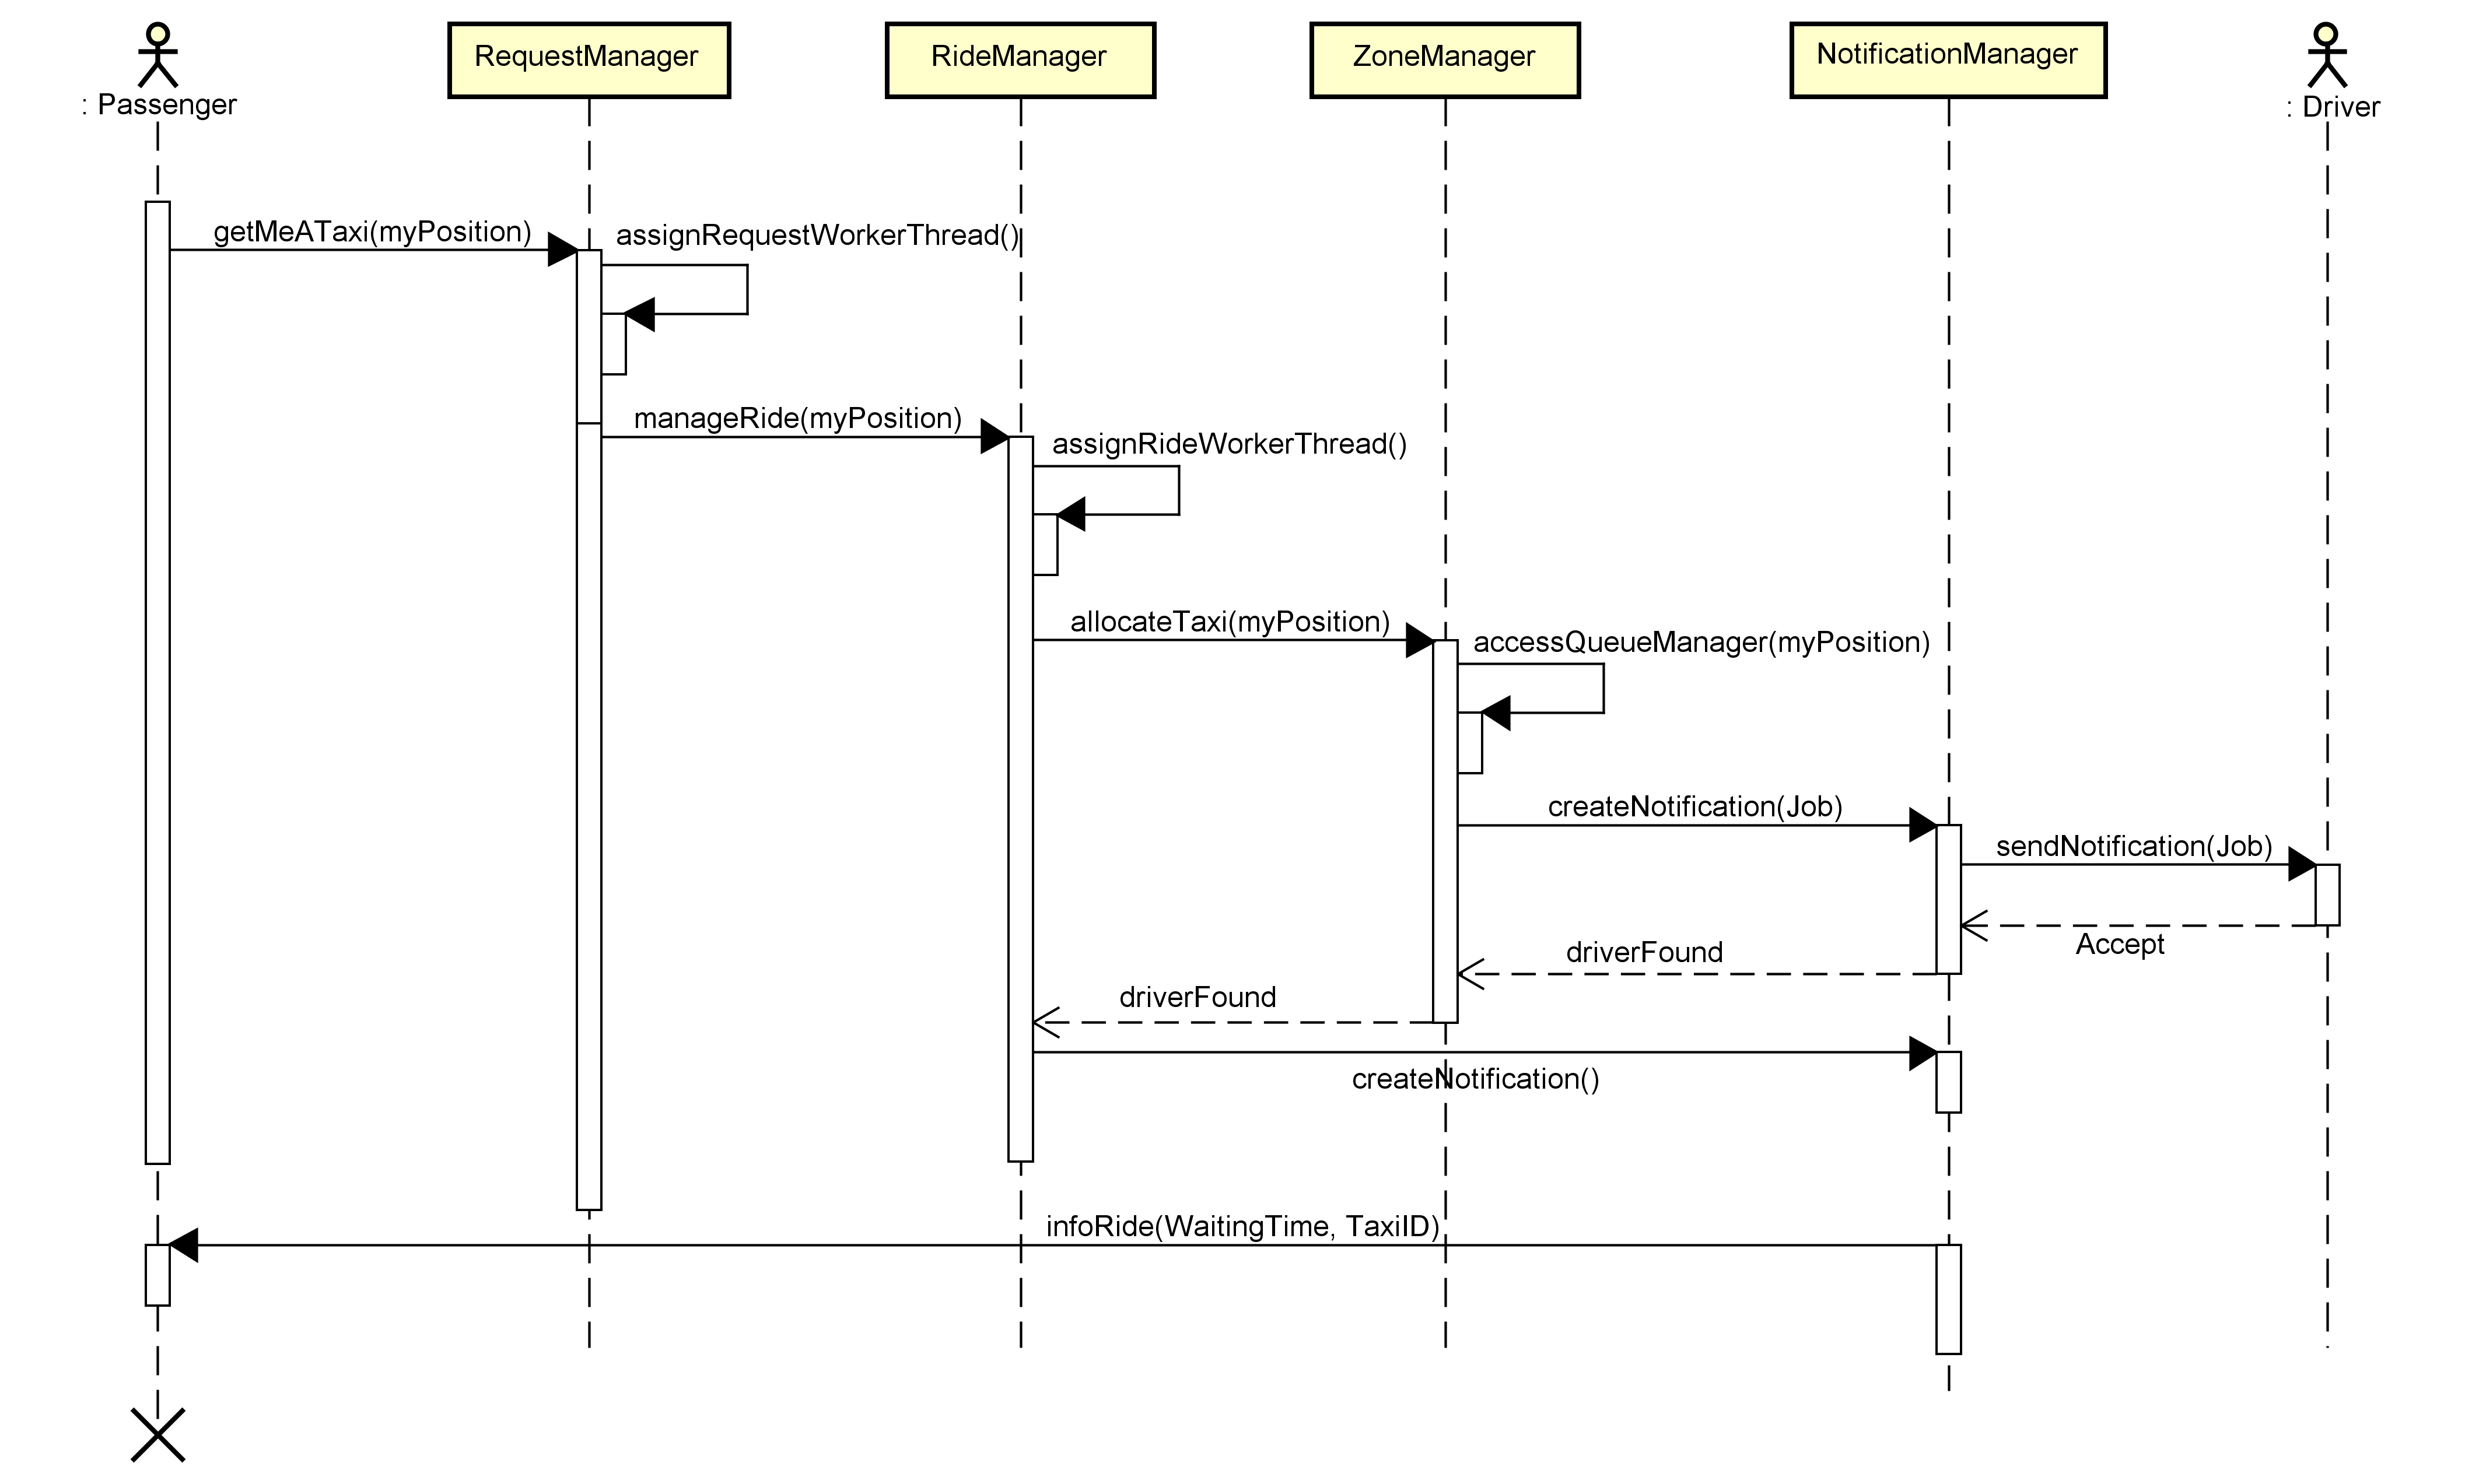
\includegraphics[keepaspectratio=true,scale=0.55]{Pictures/SDRequest}}
		\end{minipage}	
	
	\paragraph{Delete reservation} \mbox{}\\
	Below is represented the interaction between components when an user deletes a request or reservation for a taxi.	\\
		\begin{minipage}{\linewidth}
			%		\vspace*{-0.35cm}
			\makebox[\linewidth]{
				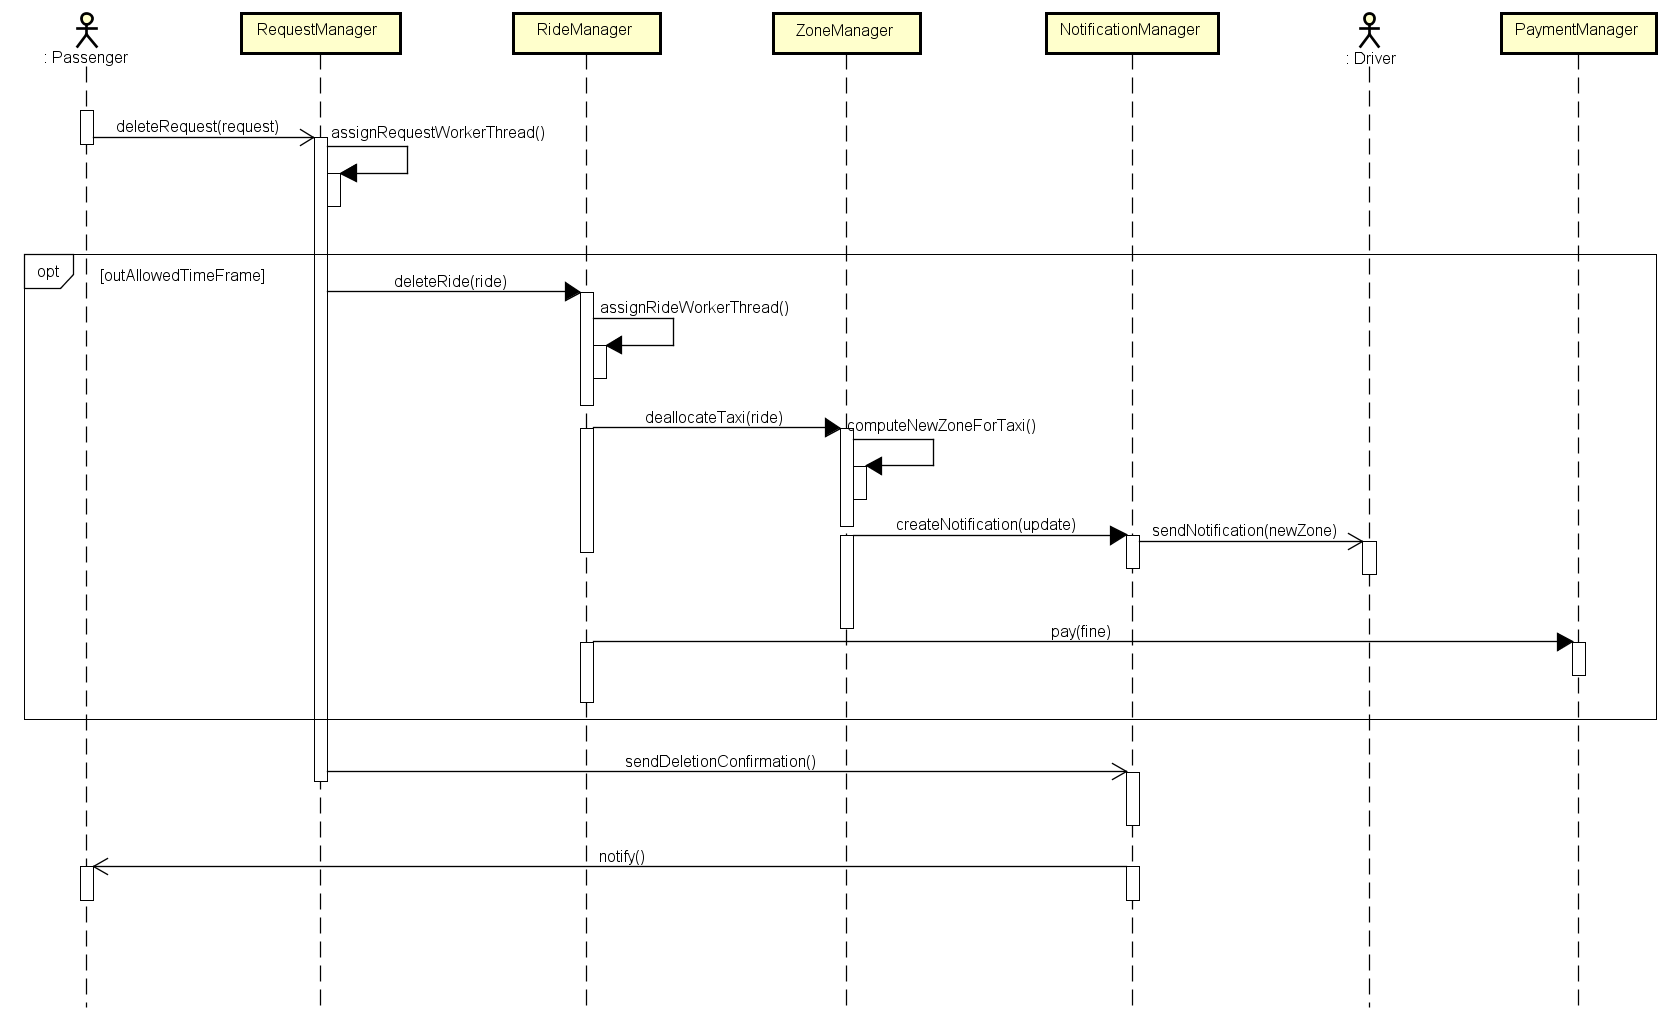
\includegraphics[keepaspectratio=true,scale=0.41]{Pictures/SDDeleteReservation}}
		\end{minipage}	
		
	\pagebreak	
	\paragraph{Driver's job proposal} \mbox{}\\
	Below is represented the interaction between components when the system has to find a driver to be assigned to a specific ride.\\		
		\begin{minipage}{\linewidth}
			%		\vspace*{-0.35cm}
			\makebox[\linewidth]{
				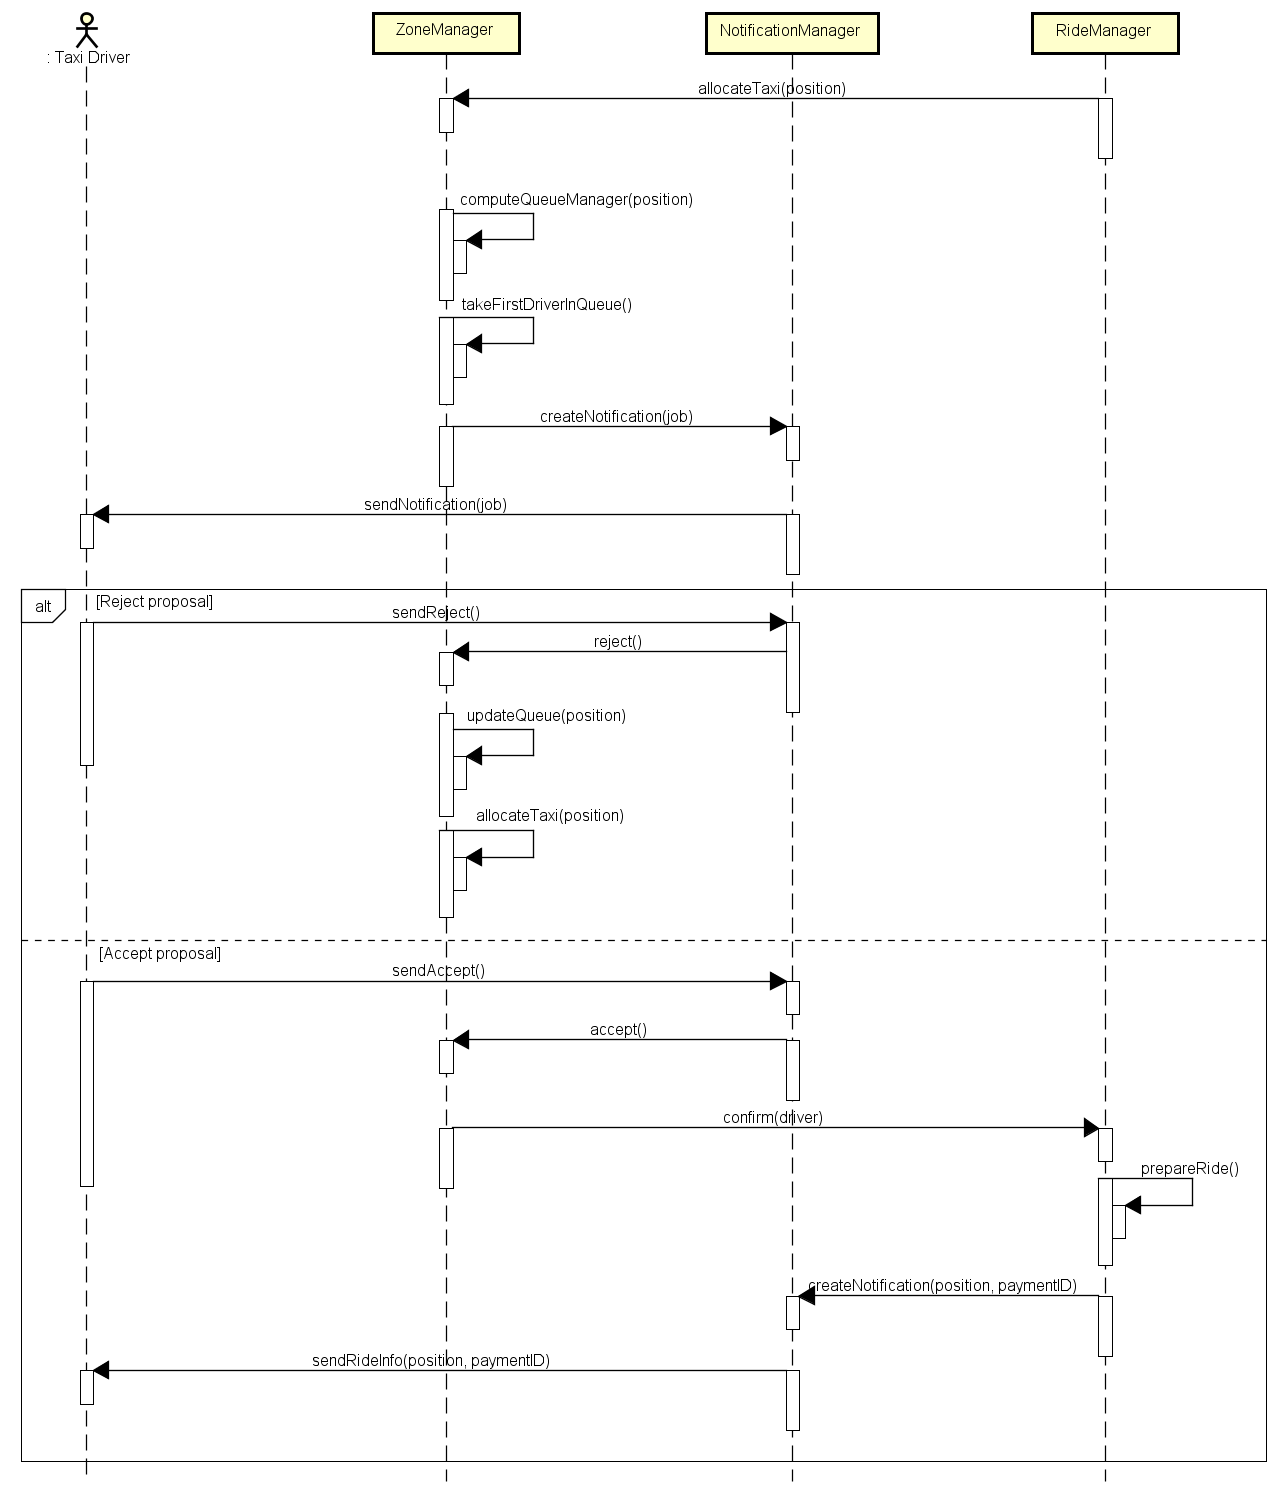
\includegraphics[keepaspectratio=true,scale=0.5]{Pictures/SDDriverJobProposal}}
		\end{minipage}	
	
	\pagebreak
	\subsection{Selected architectural styles and patterns}

	The decision of using the classical client-server architecture was straightforward. In a system like \mts{} it is important to have one single point of failure (the server) and control, with respect to distributed architectures. This decision is also compatible with the fact of having only one centralized database which sustains the whole service.\\
	For the type of interaction with clients required by the system, the ``thin client'' approach is employed; only a very simple layer of logic is implemented on the client side, for instance the acquisition of coordinated with the GPS sensor and the rendering of the graphical user interface.\\
	\mts{} relies on an ``event based'' or ``event-driven'' architecture. The system reacts to the change of state of some objects, for instance the switch of ``availability'' for the taxi driver is detected by the zone manager that operates accordingly in the respective queue. Other examples could be the change of state of a request to a modified request that must be taken into account (eg. cancellation of the request), or the consequence of the approval/refusal of a job by a driver.\\
%	 All these message-events are carried out by the NotificationManager as notifications.\\
	Some well-known software design patterns are used in the design of the system, for instance the ``Singleton'' pattern is used in the engines of the Request, Ride, Zone and Taxi Managers, while the ``Factory'' method pattern is used for the creation of instances for the workers of Account, Request and Ride Managers, respectively for every user, request and ride generated.\\
	The system is planned to be always fast and responsive, also in case of a high number of requests and accesses to the service at the same time, for this reason multithreading is highly used; parallelization to better employ the powerful server is achieved through the instantiation of multiple processes for the ProfileManager (one for every logged in user), RequestWorker (one for each request), RideWorker (one for each ride) and QueueManager (one for each zone of the city). 
		
%	\subsection{Other design decisions}

	\section{Algorithm design}
	Here are some distinctive algorithms of \mts{} presented with both pseudocode and flowchart diagrams.
	\subsection{Queue managing and taxi assignment} \label{sec:AlgoQueue}
	This algorithm depicts what happens when the system assigns a ride to a driver. It sends the proposal to the first driver of the queue in the zone where the client is located; if the driver accepts the job s/he is removed from the queue and the assignation is completed, otherwise the system forwards the request to the second driver in the queue and places the first one at the bottom of the queue. This is repeated until a driver accepts the job. \\
	This algorithm runs on the QueueManager (selected by the ZoneEngine).\\
	\lstinputlisting[language=C]{Pseudocode/QueueManager.c}
	\begin{minipage}{\linewidth}
%			\vspace*{-0.35cm}
		\makebox[\linewidth]{
		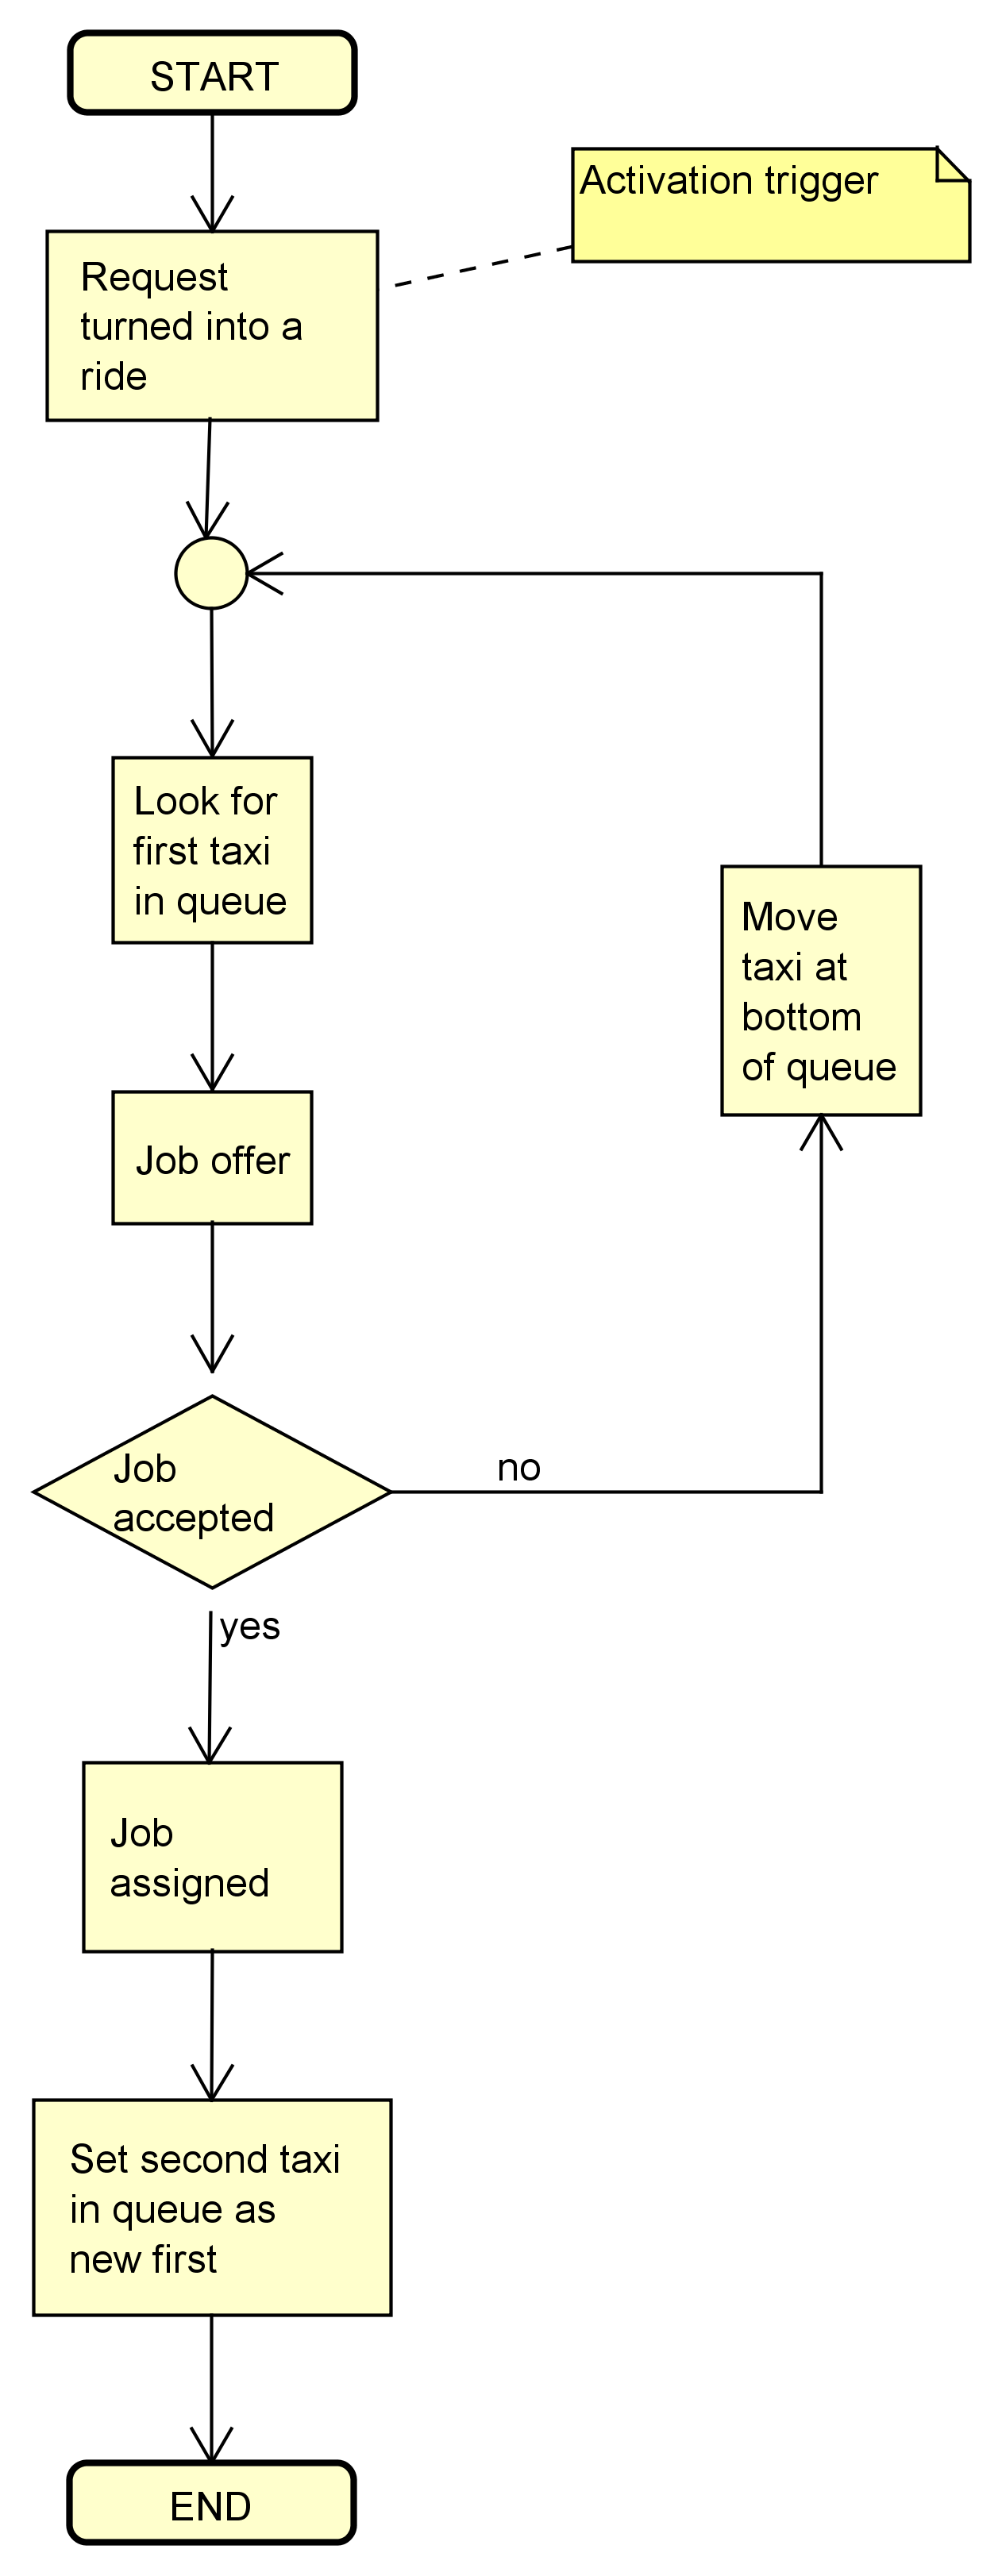
\includegraphics[keepaspectratio=true,scale=0.7]{Pictures/QueueManager}}
	\end{minipage}
	
	\pagebreak
	
	\subsection{Zone assignment} \label{sec:AlgoZone}
	This algorithm depicts what happens when the system assigns the taxi to a specific zone according to the taxi's current position obtained through the GPS sensor of the driver's phone. In particular all the zones nearby the taxi are analyzed and the zone with the shortest queue is selected. When the taxi is assigned it enters the queue at the bottom.\\
	This algorithm runs on the ZoneManager and exploits both the ZoneEngine (to select the shortest queue) and the QueueManager (to assign the taxi to the bottom of the queue).\\
	\lstinputlisting[language=C]{Pseudocode/ZoneAssignment.c}
	\begin{minipage}{\linewidth}
%			\vspace*{-0.35cm}
		\makebox[\linewidth]{
		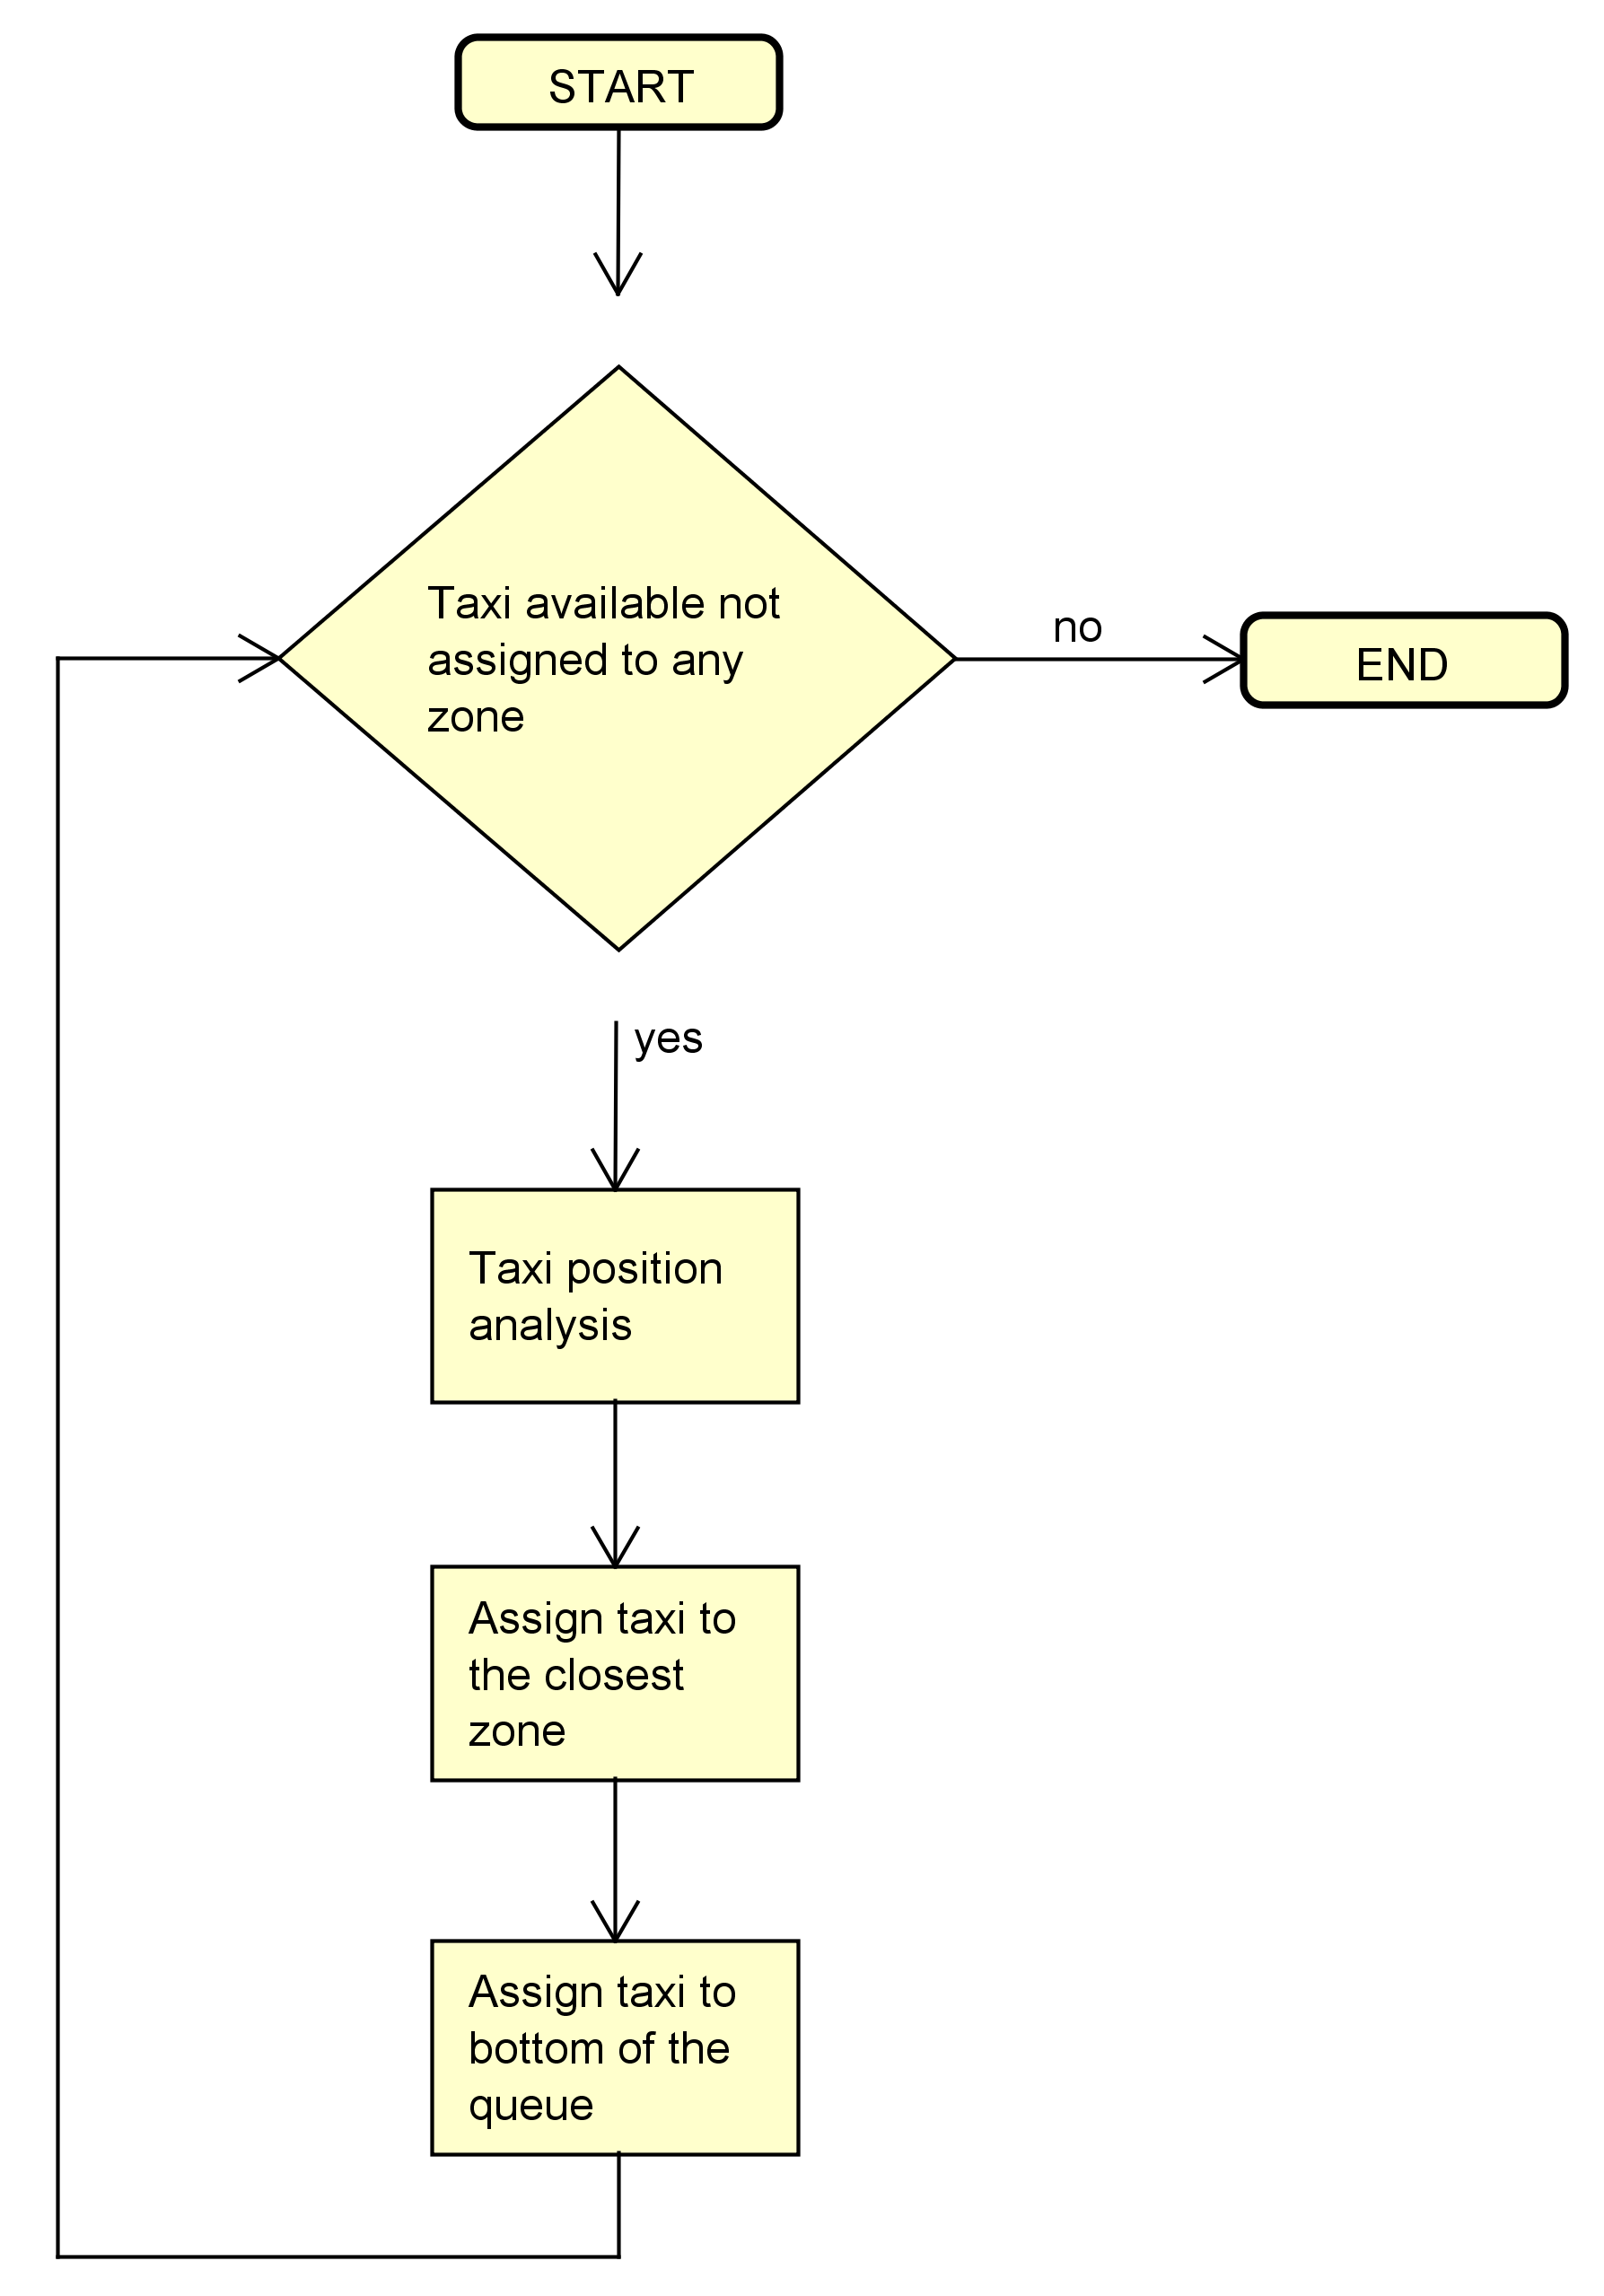
\includegraphics[keepaspectratio=true,scale=0.7]{Pictures/ZoneAssignment}}
	\end{minipage}	
	
	\pagebreak
	
	\subsection{Taxi availability} \label{sec:AlgoAvailability}
	This algorithm depicts what happens when the driver switches his/her own availability. If s/he turns it \textit{on} (\textit{waiting} to be assigned) then the system will proceed with the zone assignment according to the position, while if the driver switches the availability \textit{offline} the system will simply remove him/her from the current queue.\\
	This algorithm runs on the TaxiManager which detects the availability trigger and relies on the ZoneManager for the update of the queue according to the availability status.\\
	\lstinputlisting[language=C]{Pseudocode/Availability.c}
	\begin{minipage}{\linewidth}
%		\vspace*{-0.35cm}
		\makebox[\linewidth]{
		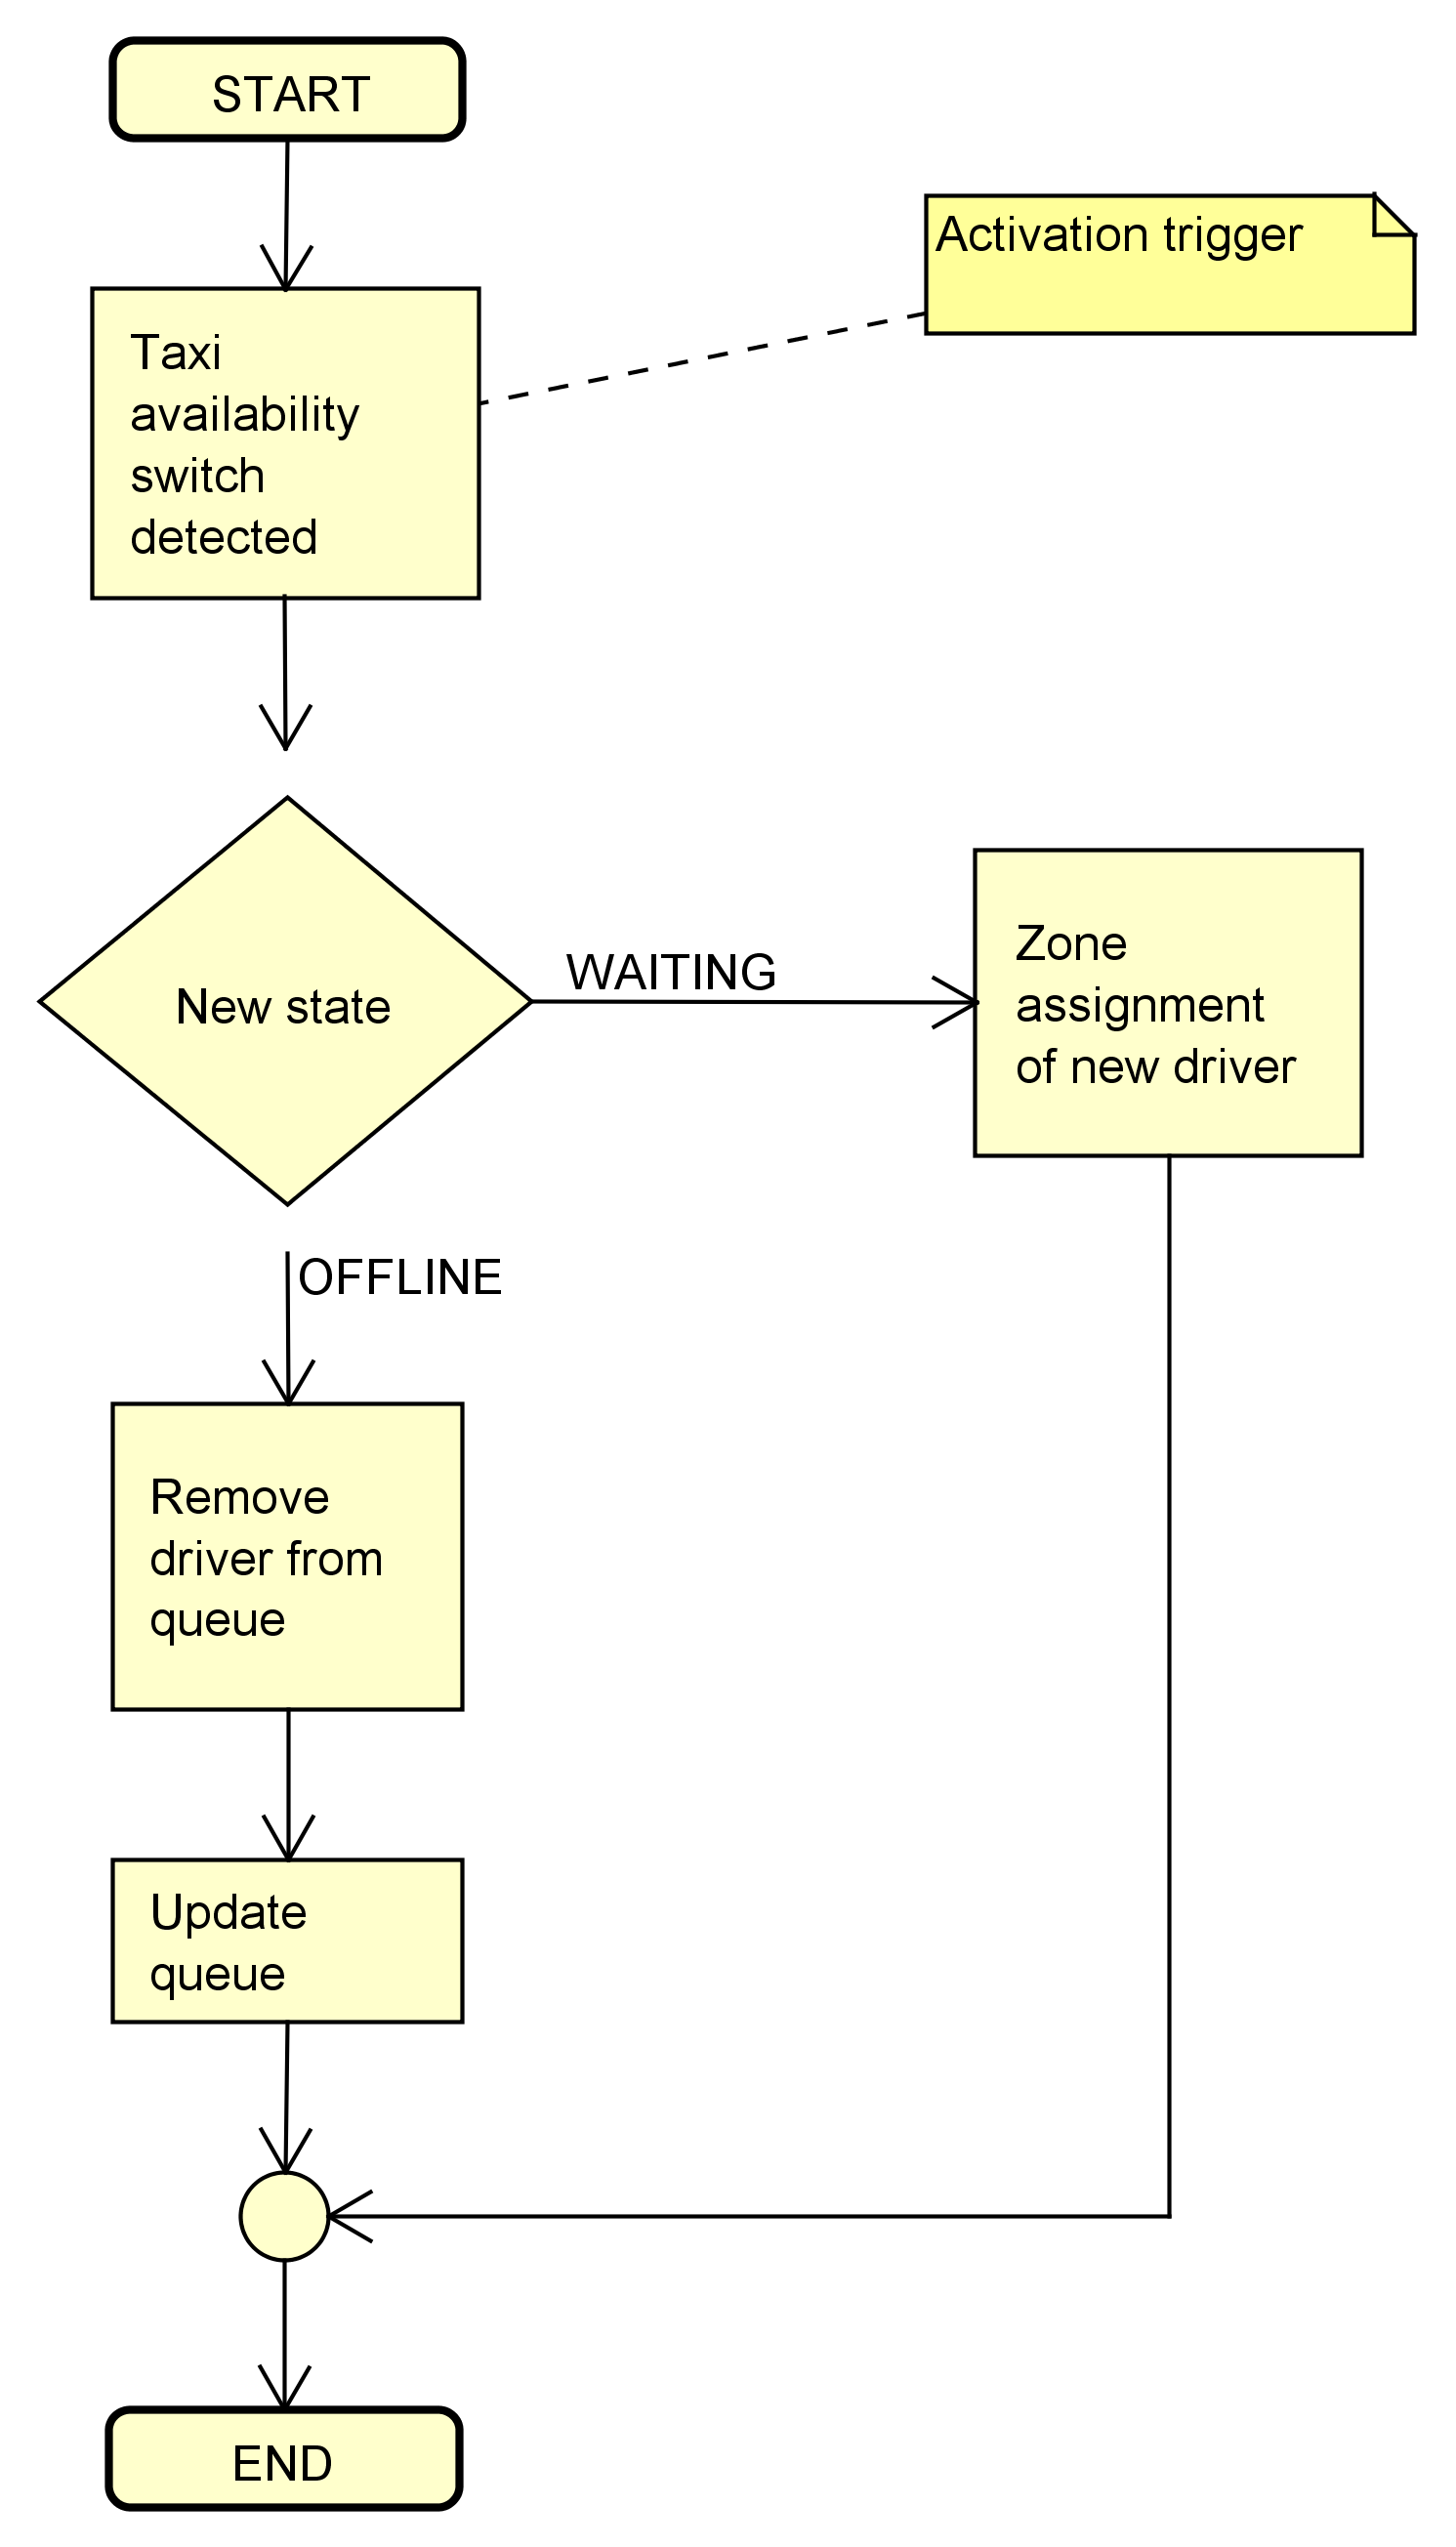
\includegraphics[keepaspectratio=true,scale=0.7]{Pictures/Availability}}
	\end{minipage}		
	
	\pagebreak
	
	\subsection{Ride creation}
	This algorithm depicts what happens when the system creates a ride based on a request or a reservation; this happens 30 seconds after the arrival of the request and 10 minutes before the meeting time for the reservation. For the request the process is straightforward and it involves the taxi allocation and the notification to all the users involved; the same is for the reservation without the sharing option. On the contrary when a ride is reserved with the possibility of sharing the trip the system must look for possible matches with same pick up and drop off zone and same date and time; if any compatible match is found then the system computes the total number of passengers. If there is enough room on the taxi for all the passengers then a shared ride is created, otherwise the system proceeds with the standard ride.\\
	This algorithm runs on the RideManager which communicates with the RequestManager to analyze matching requests, with the ZoneManager to allocate the taxi and with the NotificationManager to eventually inform all the users (passenger(s) and driver).\\
	\lstinputlisting[language=C]{Pseudocode/RideCreation.c}
	\begin{minipage}{\linewidth}
%		\vspace*{-0.35cm}
		\makebox[\linewidth]{
		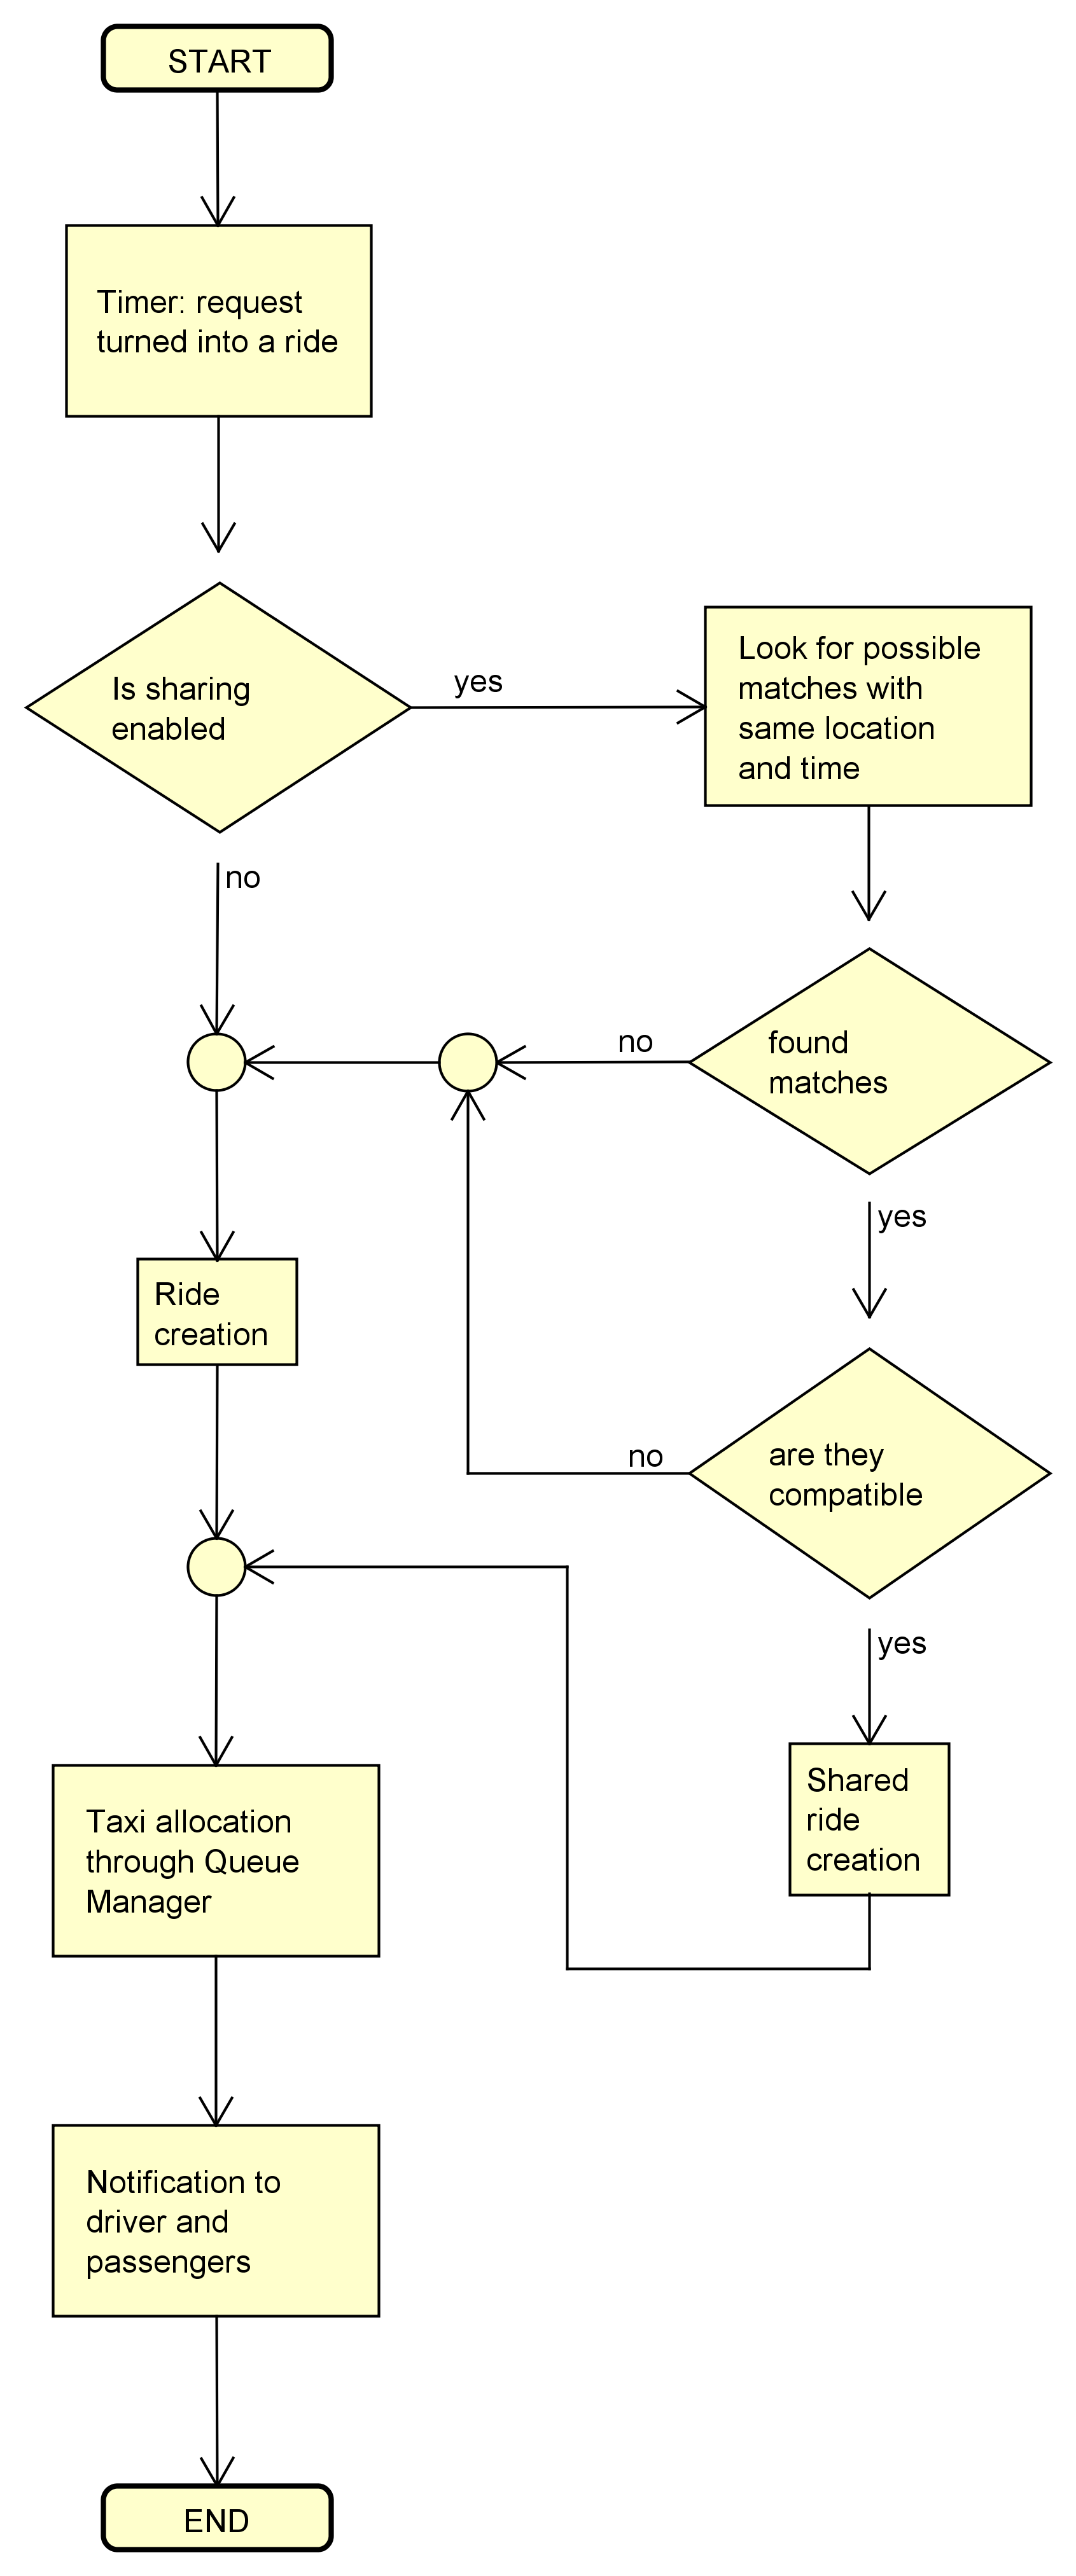
\includegraphics[keepaspectratio=true,scale=0.7]{Pictures/RideCreation}}
	\end{minipage}		
	
	\subsection{Payment}
	This algorithm represents the way the system deducts money from the passenger's credit card. It can collect the standard fare computed on the distance covered on the taxi or a penalty fee. The latter is only applied when the user deletes (or modifies) a request/reservation beyond the allowed time frame, that is within 30 seconds after the application for the request and until 10 minutes before the meeting time for the reservation (basically once the ride is generated if the user deletes it s/he will incur in the penalty fee). A cancellation within the allowed time window does not involve any penalty fine.\\
	When the ride is carried out successfully the fare is computed on the basis of the type of ride \textit{shared} or regular.\\
	This algorithm runs on the PaymentManager which communicates with the RideManager.\\
	\lstinputlisting[language=C]{Pseudocode/Payment.c}
	\begin{minipage}{\linewidth}
%		\vspace*{-0.35cm}
		\makebox[\linewidth]{
		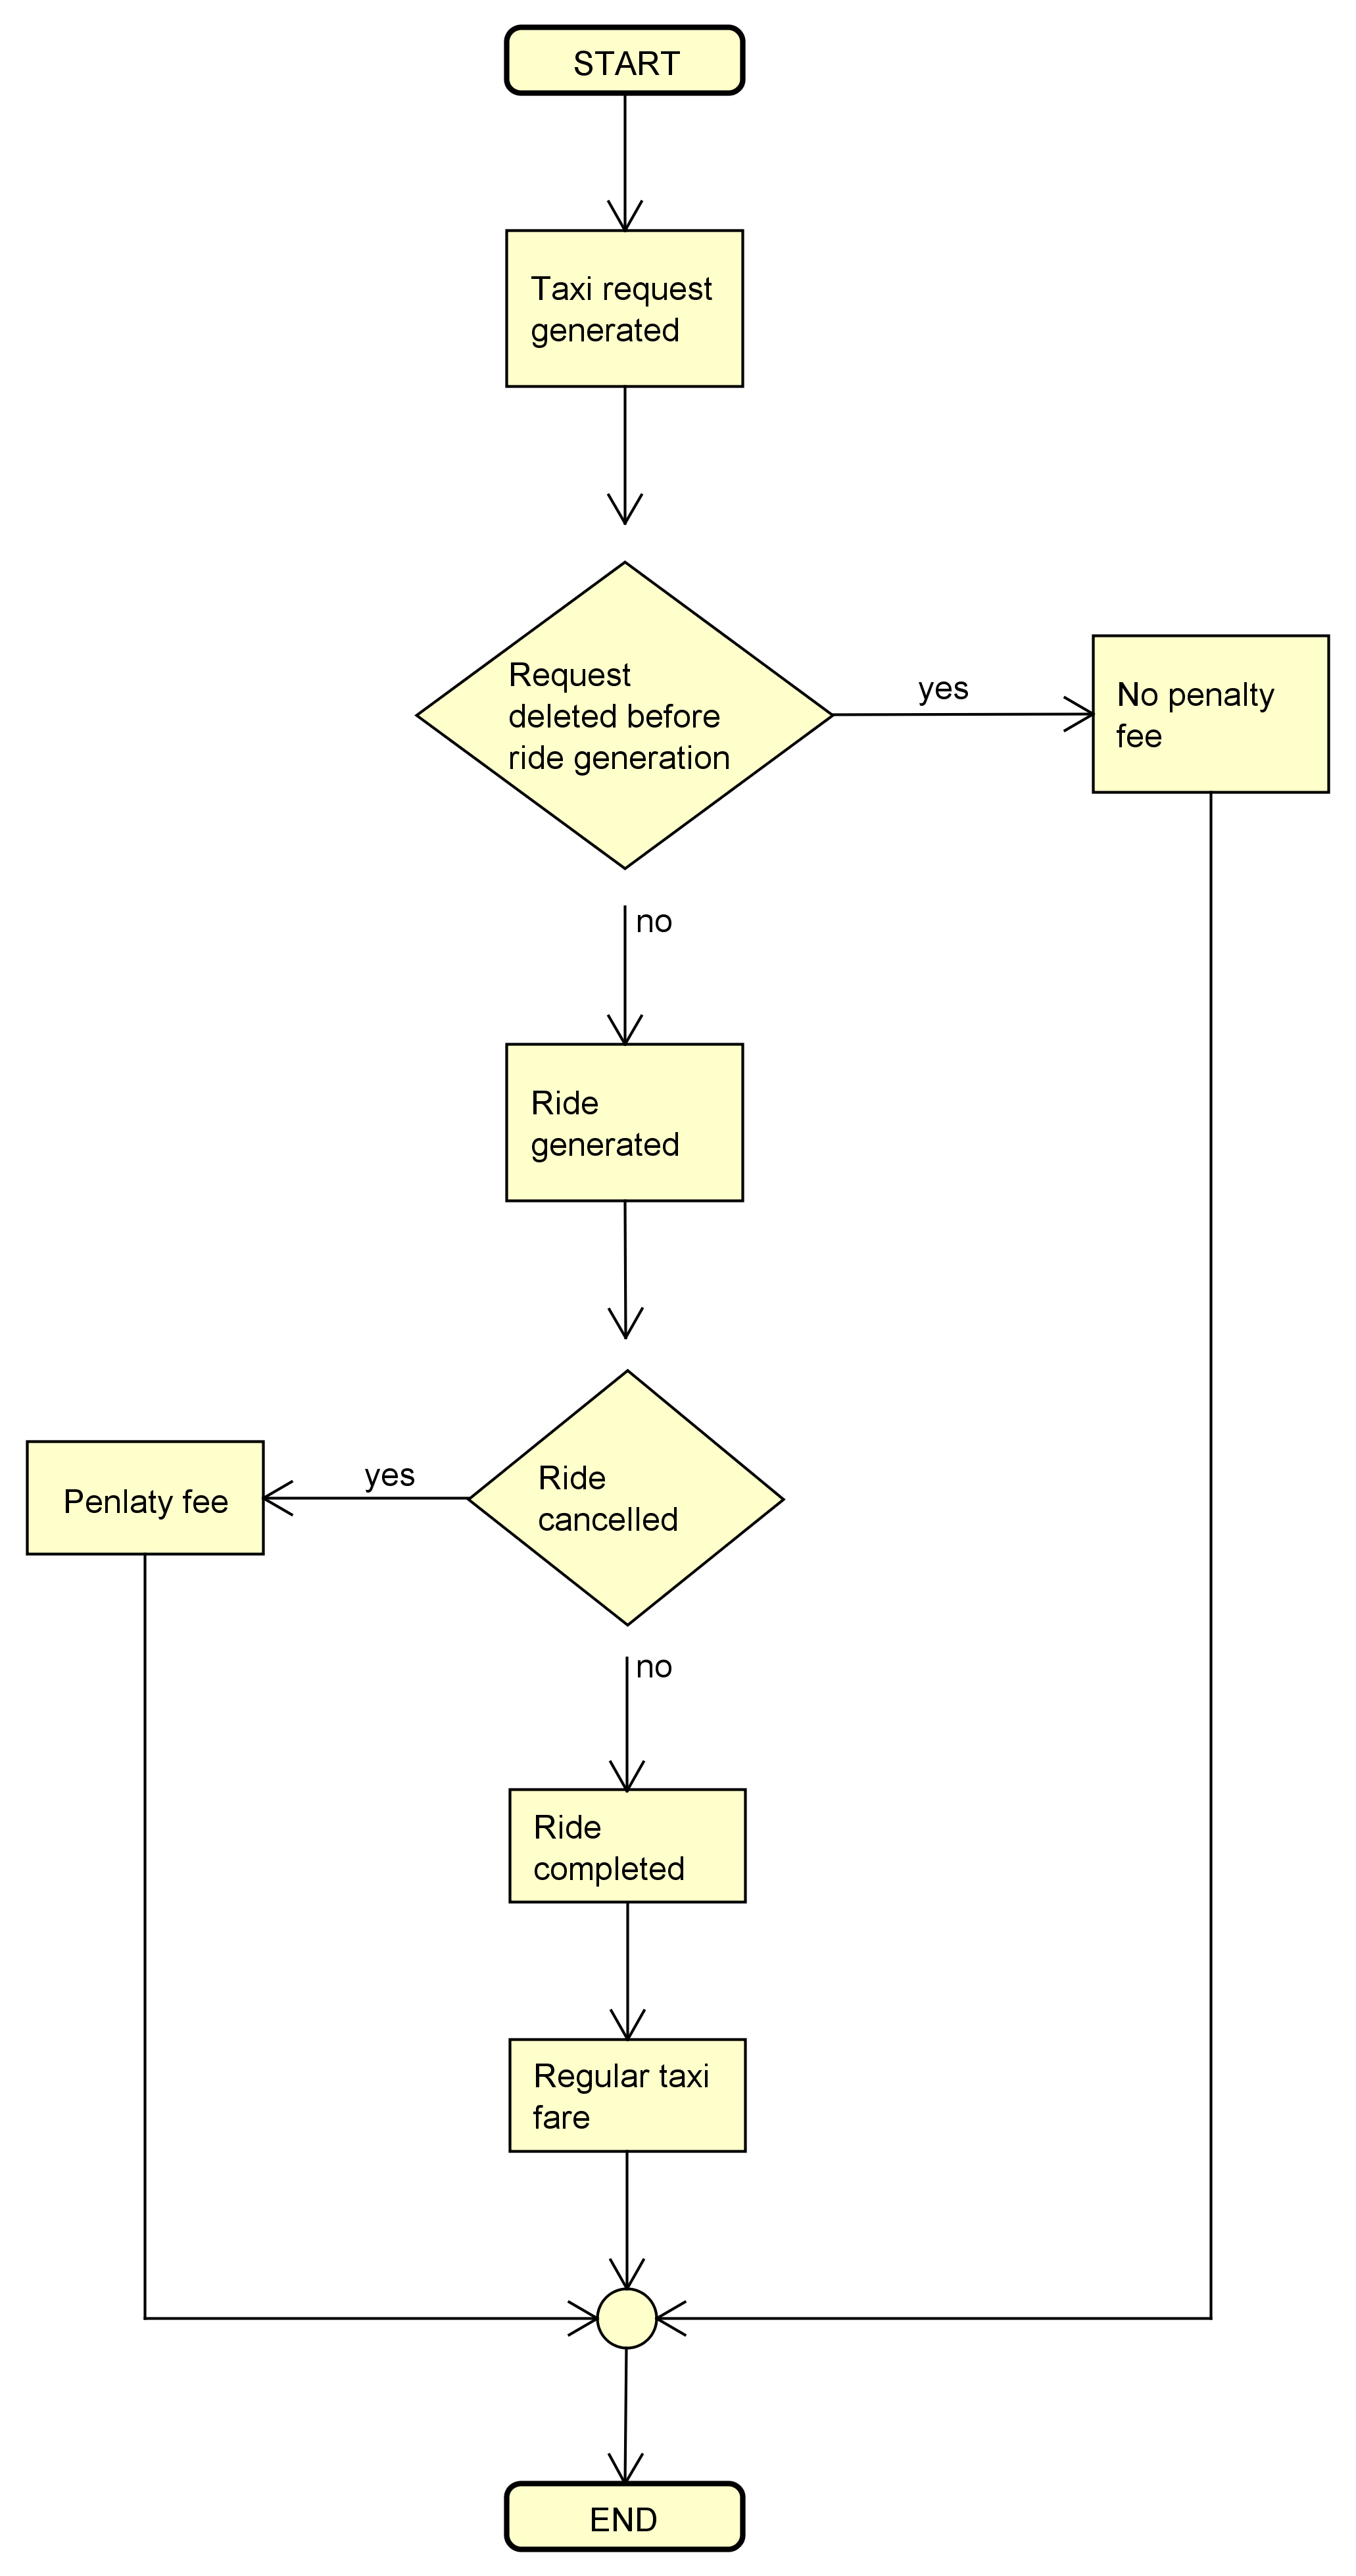
\includegraphics[keepaspectratio=true,scale=0.7]{Pictures/Payment}}
	\end{minipage}	
	
	\section{User Interface Design}
	This section is the same featured in the RASD.\\
	Shown below are some mock-ups that preview the user interface of the main features the system shall provide.
	
	\pagebreak
	\paragraph{Sign-up} This page presents the sign up form for the clients. The user will need to provide his/her personal data, home and email addresses, phone number, favorite payment option, favorite notification type.
	\begin{center}
		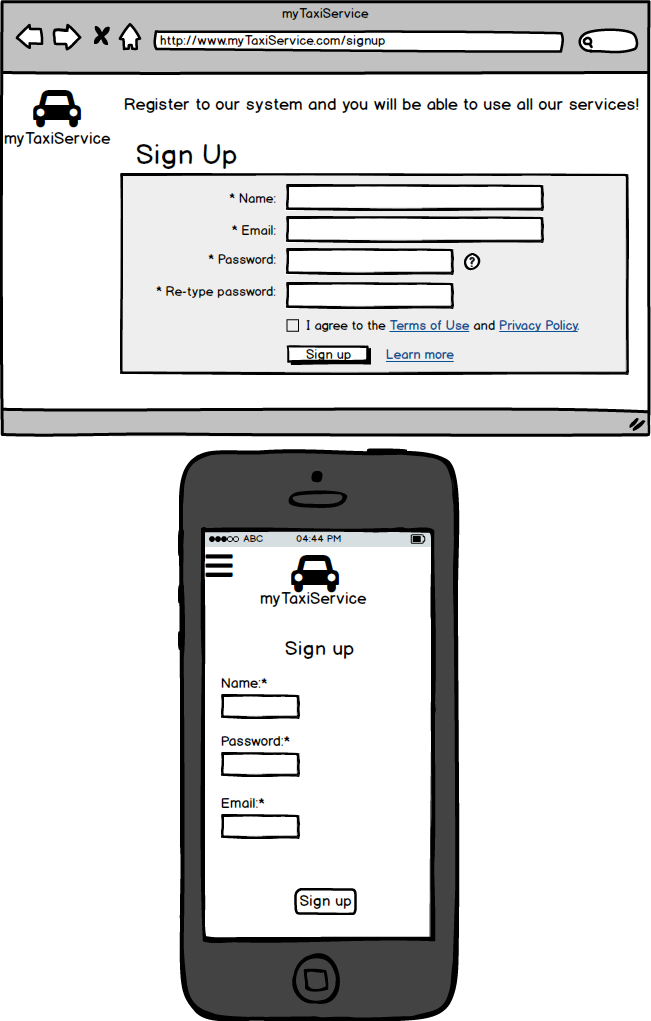
\includegraphics[width=0.9\linewidth]{Pictures/Signup}
	\end{center}
	\pagebreak
	
	\paragraph{Login} This page shows the login form for the final users.
	\begin{center}
		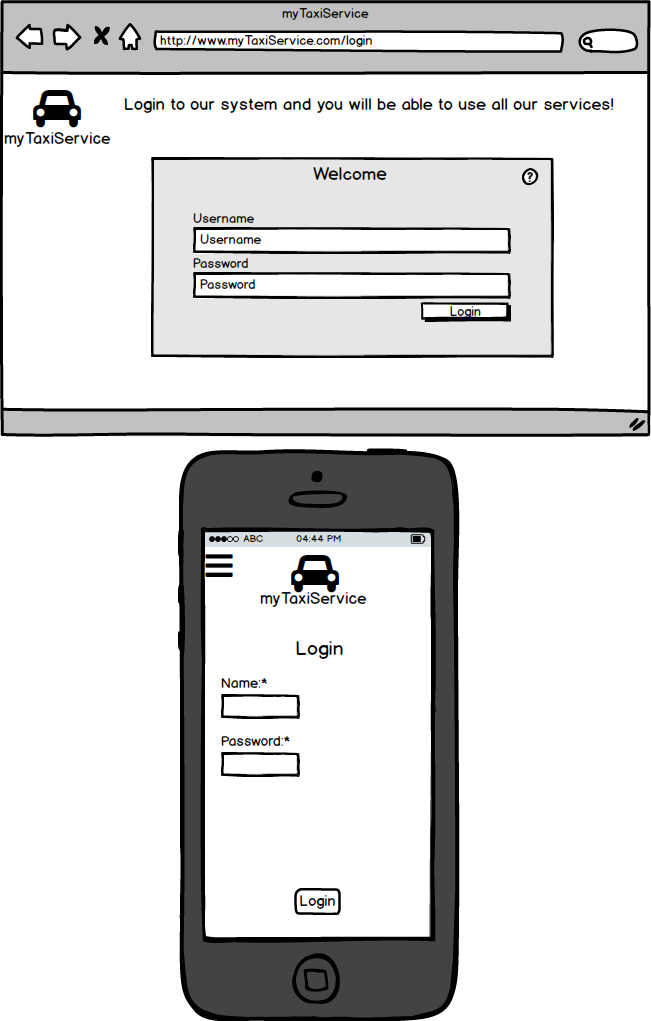
\includegraphics[width=0.9\linewidth]{Pictures/Login}
	\end{center}
	\pagebreak
	
	\pagebreak
	\paragraph{Call a taxi} The user can ask for a taxi providing the pickup location through a complete address or through the automatic detection of his/her location thanks to the browser or the GPS. The user can also choose from an history of ``recent addresses''.
	\begin{center}
		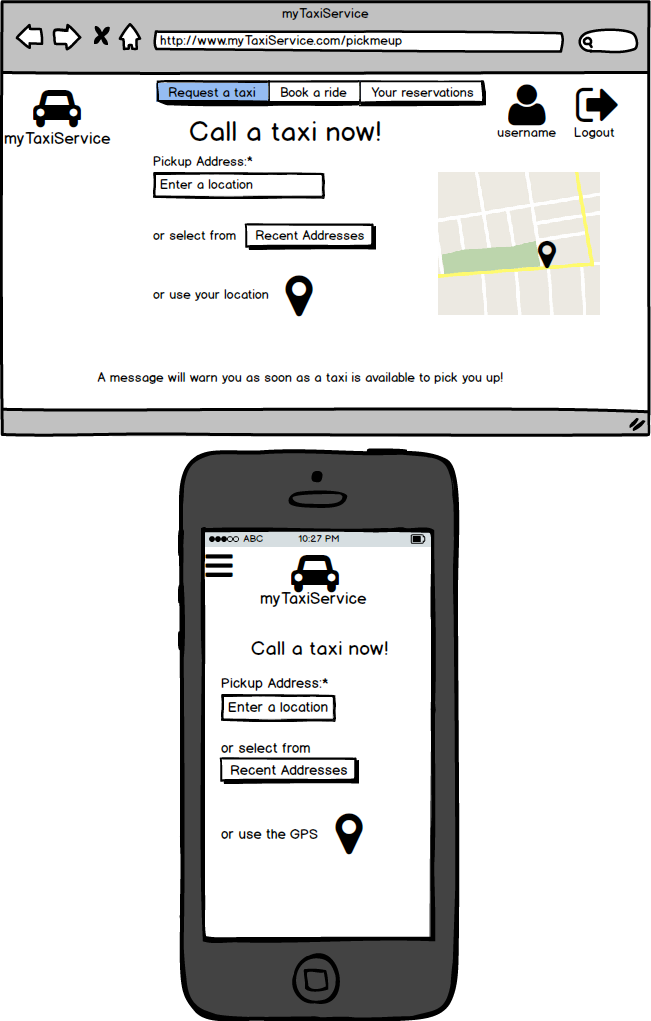
\includegraphics[width=0.9\linewidth]{Pictures/CallATaxi}
	\end{center}
	\pagebreak
	
	\paragraph{Plan a ride} The user can plan a ride in advance providing the pickup and drop off locations, the date and time, the willingness to share the ride and the number of passengers.
	\begin{center}
		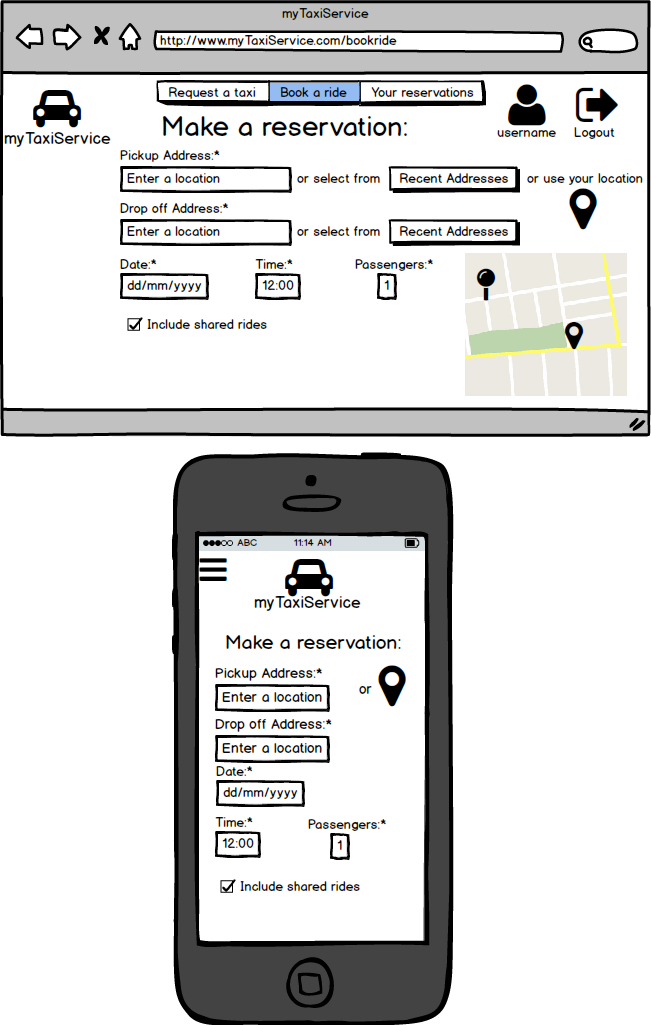
\includegraphics[width=0.9\linewidth]{Pictures/PlanAndBookARide}
	\end{center}
	\pagebreak
	
	\paragraph{Your reservations} The user can see both the active reservations and the past ones. S/he can edit the active reservations within the established time frame before the meeting time.
	\begin{center}
		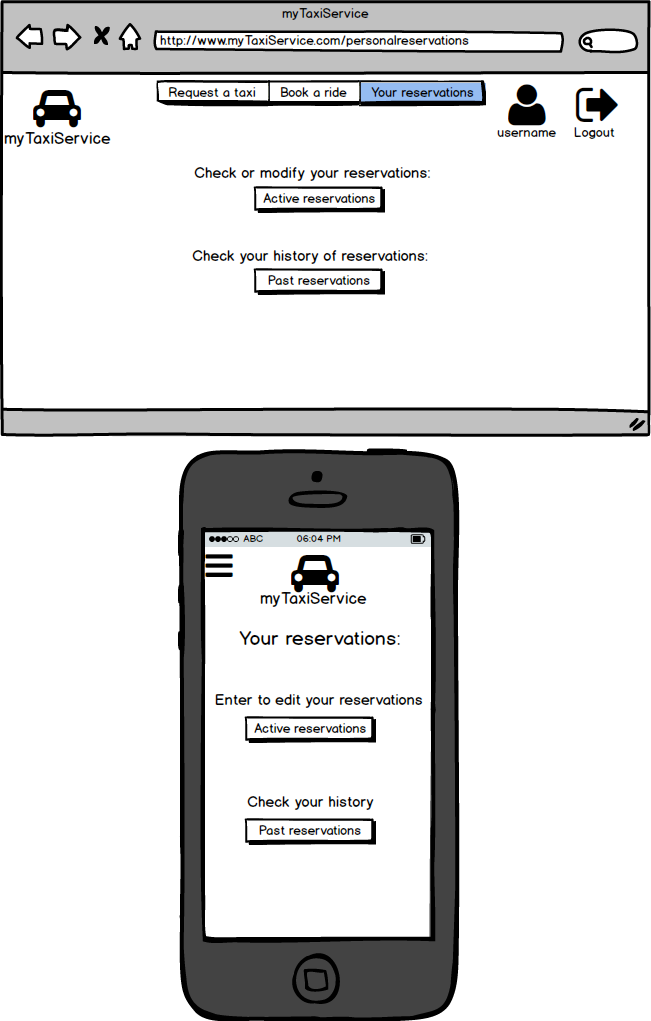
\includegraphics[width=0.9\linewidth]{Pictures/YourReservations}
	\end{center}
	\pagebreak
	
	\paragraph{Your profile} The user can edit the personal profile modifying the password, phone number, email address, permanent address, payment method and notification type.
	\begin{center}
		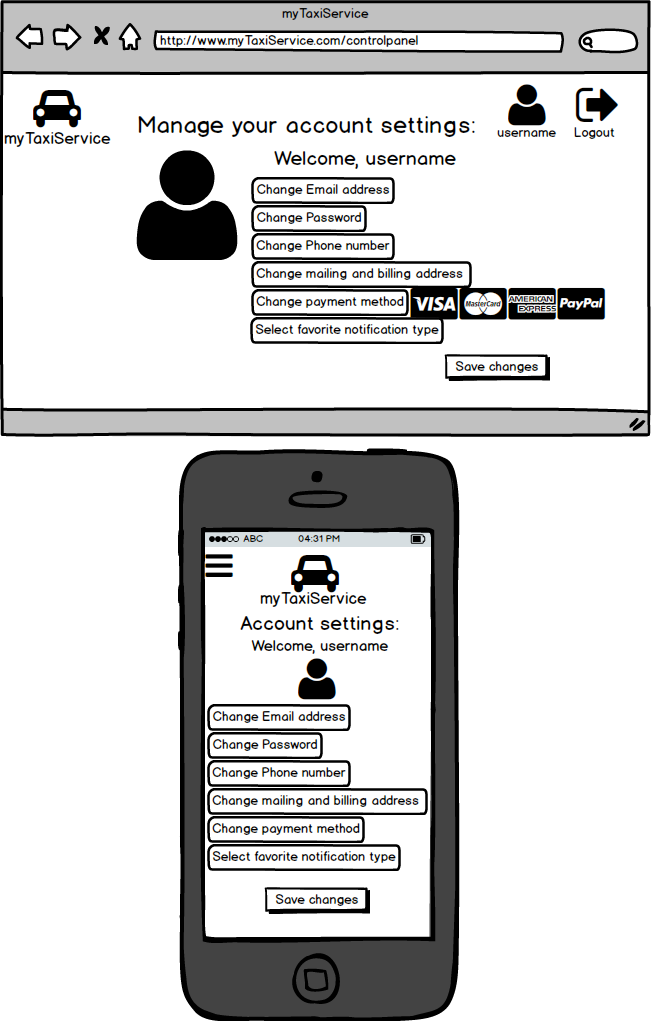
\includegraphics[width=0.9\linewidth]{Pictures/AccountPage}
	\end{center}
	\pagebreak
	
	\paragraph{Manage jobs} The taxi driver's home page: s/he can accept or reject the requests forwarded by the system and set her/his own ``availability''.
	\begin{center}
		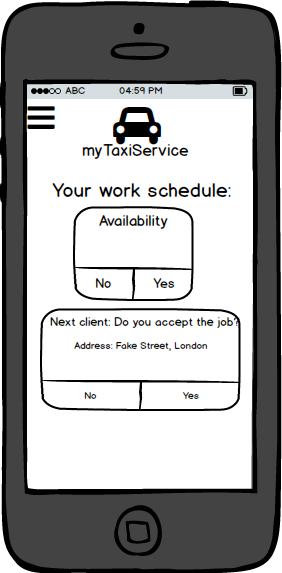
\includegraphics[width=0.4\linewidth]{Pictures/DriverPage}
	\end{center}
	\pagebreak
	
	\paragraph{Administrator panel} The administrator's home page: s/he can monitor the whole system or manage taxi drivers inserting new employees in the system DB or modifying/deleting existing ones.
	\begin{center}
		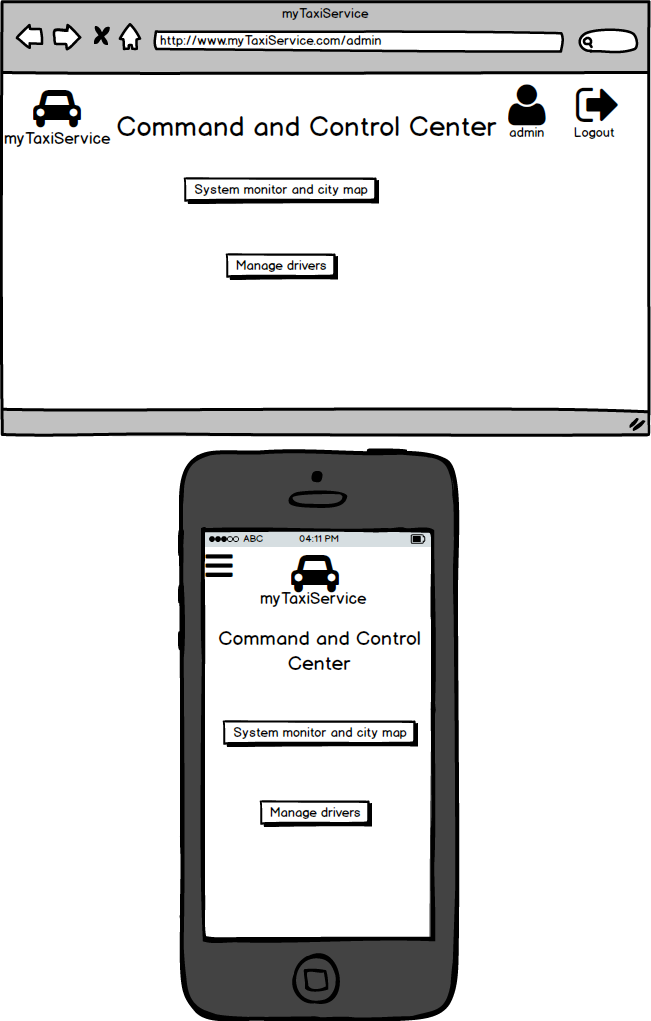
\includegraphics[width=0.9\linewidth]{Pictures/AdminPage}
	\end{center}
	\pagebreak	
	
	\section{Requirements Traceability}
	The following table shows the mapping between the required functionalities of the system and the components used to implement and satisfy them.
	\begin{center}
		\begin{longtable}{| p{7cm} | p{8cm} |}\hline
			\centerline{\textbf{Goals}} & \centerline{\textbf{Assigned component}} \\\hline
			{[}G2{]} The system has to guarantee a fair management of the queues in each taxi zone. & The QueueManager (inner component of ZoneManager) runs the algorithm described in the previous section (see section~\ref{sec:AlgoQueue}) to guarantee a fair management of the queue, with the mechanism previously agreed.\\\hline
			{[}G3{]} The system has to assign taxis to the zones in such a way that the queues are never empty. & The ZoneManager runs the algorithm described in the previous section (see section~\ref{sec:AlgoZone}) to guarantee the presence of at least one taxi in every queue.\\\hline
			{[}G4{]} The system has to allocate a taxi for each request or reservation. & The RideManager is in charge of the taxi assignation for every ride.\\\hline
			{[}G5{]} The system has to notify the users, both passengers and taxi drivers, about updates on taxi requests and rides in which they are involved. & The NotificationManager receives the updates to be sent to the users from the other components.\\\hline
			{[}G6{]} The system has to offer public APIs to enable the possibility to develop additional services on top of the basic ones. & The different components offer the PublicAPI interfaces that allow external services to access the system, send requests and view the real-time position of the taxis.\\\hline
			{[}G7{]} The passenger shall be able to sign up to the service. & The SignUpManager (inner component of AccountManager) offers the SignUp interface to the Visitor.\\\hline
			{[}G8{]} The passenger shall be able to login to the service. & The LoginManager (inner component of AccountManager) offers the Login interface (through the facade pattern) to satisfy this requirement.\\\hline	
			{[}G9{]} The passenger shall be able to request a taxi. & The RequestHandler (inner component of RequestManager) offers the ManageRequest interface (through the facade pattern) to the Passenger.\\\hline
			{[}G10{]} The passenger shall be able to delete a taxi request. & The RequestHandler (inner component of RequestManager) offers the ManageRequest interface (through the facade pattern) to the Passenger.\\\hline	
			{[}G11{]} The passenger shall be able to create a reservation for a taxi ride. & The RequestHandler (inner component of RequestManager) offers the ManageRequest interface to fulfill this task.\\\hline
			{[}G12{]} The passenger shall be able to modify or delete a taxi reservation.	& The RequestHandler (inner component of RequestManager) provides the ManageRequest interface to fulfill this task.\\\hline
			{[}G13{]} The passenger shall be able to enable taxi sharing option. & The RequestHandler (inner component of RequestManager) receives a completely customized reservation.\\\hline
			{[}G14{]} The passenger shall be able to see historical data on his taxi rides. & The RequestEngine (inner component of RequestManager) offers the History interface to fulfill this requirement.\\\hline
			{[}G15{]} Taxi drivers shall be able to log in to the service. & The LoginManager (inner component of AccountManager) is in charge of this task.\\\hline	
			{[}G16{]} Taxi drivers must inform the system about their availability. & The TaxiManager runs the algorithm described in the previous section (see section~\ref{sec:AlgoAvailability}) to guarantee the response of the system according to the driver's availability. It relies on the ZoneManager to assign the taxis to the queues or to the jobs, or to remove them when they are offline.\\\hline
			{[}G17{]} Taxi drivers must confirm if they are going to take care of a certain call. & The QueueManager (inner component of ZoneManager) is in charge of this interaction.\\\hline
			{[}G18{]} The administrator shall be able to add, edit and delete taxi drivers in the system. & The ProfileManager (inner component of AccountManager) offers the ManageTaxiDriver interface to the Administrator.\\\hline
			{[}G19{]} The administrator shall be able to manage and supervise the operation of the whole system, including the real-time situation of all the queues and of the taxis. & The ZoneEngine (inner component of ZoneManager) offers the Monitor interface to the Administrator.\\\hline
			
		\end{longtable}
	\end{center} 
	
	\pagebreak
	\section{References}
	\begin{itemize}
		\item Text: \textit{Principi di Ingegneria del Software} 5ed, Roger S. Pressman, McGraw-Hill
		\item Material from Wikipedia
		\begin{itemize}
			\item Thin client: \href{https://en.wikipedia.org/wiki/Thin_client}{https://en.wikipedia.org/wiki/Thin\_client}
			\item Event-driven architecture: \href{https://en.wikipedia.org/wiki/Event-driven_architecture}{https://en.wikipedia.org/wiki/Event-driven\_architecture}
			\item Factory method pattern: \href{https://en.wikipedia.org/wiki/Factory_method_pattern}{https://en.wikipedia.org/wiki/Factory\_method\_pattern}
			\item Singleton pattern: \href{https://en.wikipedia.org/wiki/Singleton_pattern}{https://en.wikipedia.org/wiki/Singleton\_pattern}
			\item Facade pattern: \href{https://en.wikipedia.org/wiki/Facade_pattern}{https://en.wikipedia.org/wiki/Facade\_pattern}
			\item Deployment diagram:
			\href{https://en.wikipedia.org/wiki/Deployment_diagram}{https://en.wikipedia.org/wiki/Deployment\_diagram}
		\end{itemize}
	\end{itemize}
	
	
	\section{Appendix}
	
	\subsection{Software and tools used}
	\begin{itemize}
		\item TeXstudio 2.10.4 (http://www.texstudio.org/) to redact and format this document.
		\item Astah Professional 7.0 (http://astah.net/editions/professional): to create Use
		Cases Diagrams, Sequence Diagrams, Class Diagrams and State Machine	Diagrams.
		\item Microsoft Office Visio Professional 2016
%		\item Balsamiq Mockups 3.2.4 (http://balsamiq.com/products/mockups/) to create the mockups.
	\end{itemize}
	
	\subsection{Hours of work} The time spent to redact this document:
	\begin{itemize}
		\item Baldassari Alessandro: 30 hours.
		\item Bendin Alberto: 30 hours.
		\item Giarola Francesco: 30 hours.
	\end{itemize}
\end{document}